\chapter{Pair background}
\label{Appendix:Pairs}

This appendix gives additional details on the simulation study of the pair background induced by beam-beam interactions, described in Chapter~\ref{PairBkg}.

\section{GuineaPig event generation}
\label{Appendix:Pairs:GuineaPig}
The parameters used as input for \guineapig are given in this section.
For detailed explanations of the \guineapig parameters, refer to the \guineapig manual~\cite{GuineaPigMan}.
\\The parameters are provided in a file called ``acc.dat''.
Its content must have a certain format, for which an example showing the nominal parameters used for the ILC500 stage is following:\vspace*{0.1cm}\\
\texttt{\$ACCELERATOR:: ILC-500GeV\\
\{energy=250.0; particles=2.0; beta\_x=11.0; beta\_y=0.48;\\
emitt\_x=10.0; emitt\_y=0.035; sigma\_z=300.0; f\_rep=5.0; n\_b=1312;\\
charge\_sign=-1; scale\_step=1.0; waist\_y=250;\\
espread.1=0.00124; espread.2=0.0007; which\_espread=3;\}\\
\$PARAMETERS:: par\_pairs\\
\{n\_z=12; n\_t=6; n\_m=80000; cut\_z=3.5*sigma\_z.1; n\_x=256; n\_y=256;\\
cut\_x=4*sigma\_x.1; cut\_y=4*sigma\_y.1; pair\_ecut=1e-3; pair\_q2=2;\\
beam\_size=1; grids=7; store\_beam=1; do\_pairs=1; track\_pairs=1;\\
store\_pairs=1; do\_photons=1; store\_photons=1; do\_hadrons=1;\\
do\_jets=1; do\_coherent=1; electron\_ratio=1; photon\_ratio=1;\\
do\_eloss=1; do\_espread=1; rndm\_seed=1; rndm\_load=0; rndm\_save=0;\}
}
\vspace*{0.2cm}\\For the ILC250 stage, the parameters are exchanged with according the beam parameter values taken from Table~\ref{tab:ILC_parameters}.
\newpage
\section{\sid occupancy for the ILC250 parameter sets}
\label{Appendix:Pairs:ILC250_occupancy}

\subsection{Pair background occupancy in the \sid vertex detector}
\begin{figure}[htbp]
 \centering
   \begin{subfigure}[b]{0.49\textwidth}
   \centering
    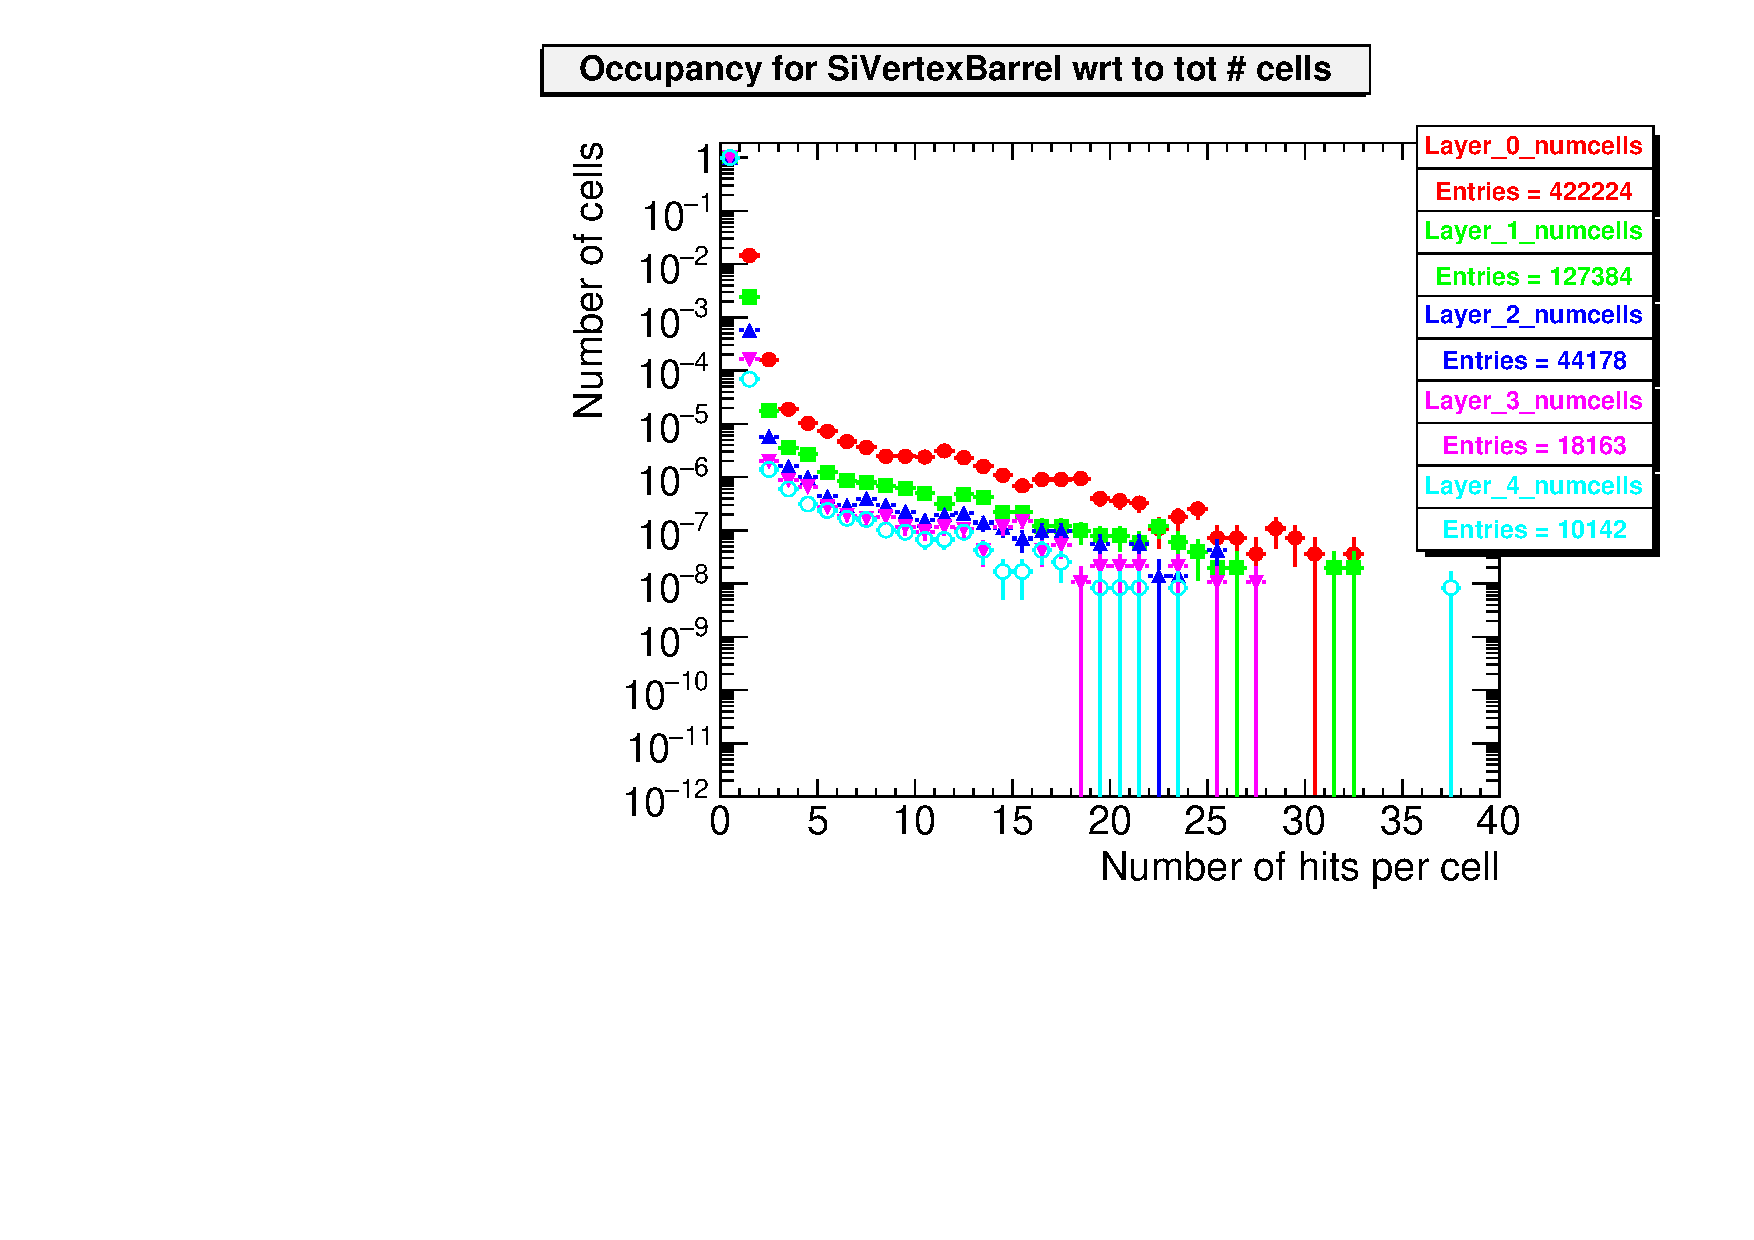
\includegraphics[width=\textwidth]{Figures/Pairs/Appendix/occupancy_numcells_SiVertexBarrel_ILC250_TDR_corrected_Barrel_size.pdf}
   \caption{Set (TDR), normalized occupancy}
   \end{subfigure}
   \hfill
    \begin{subfigure}[b]{0.49\textwidth}
   \centering
    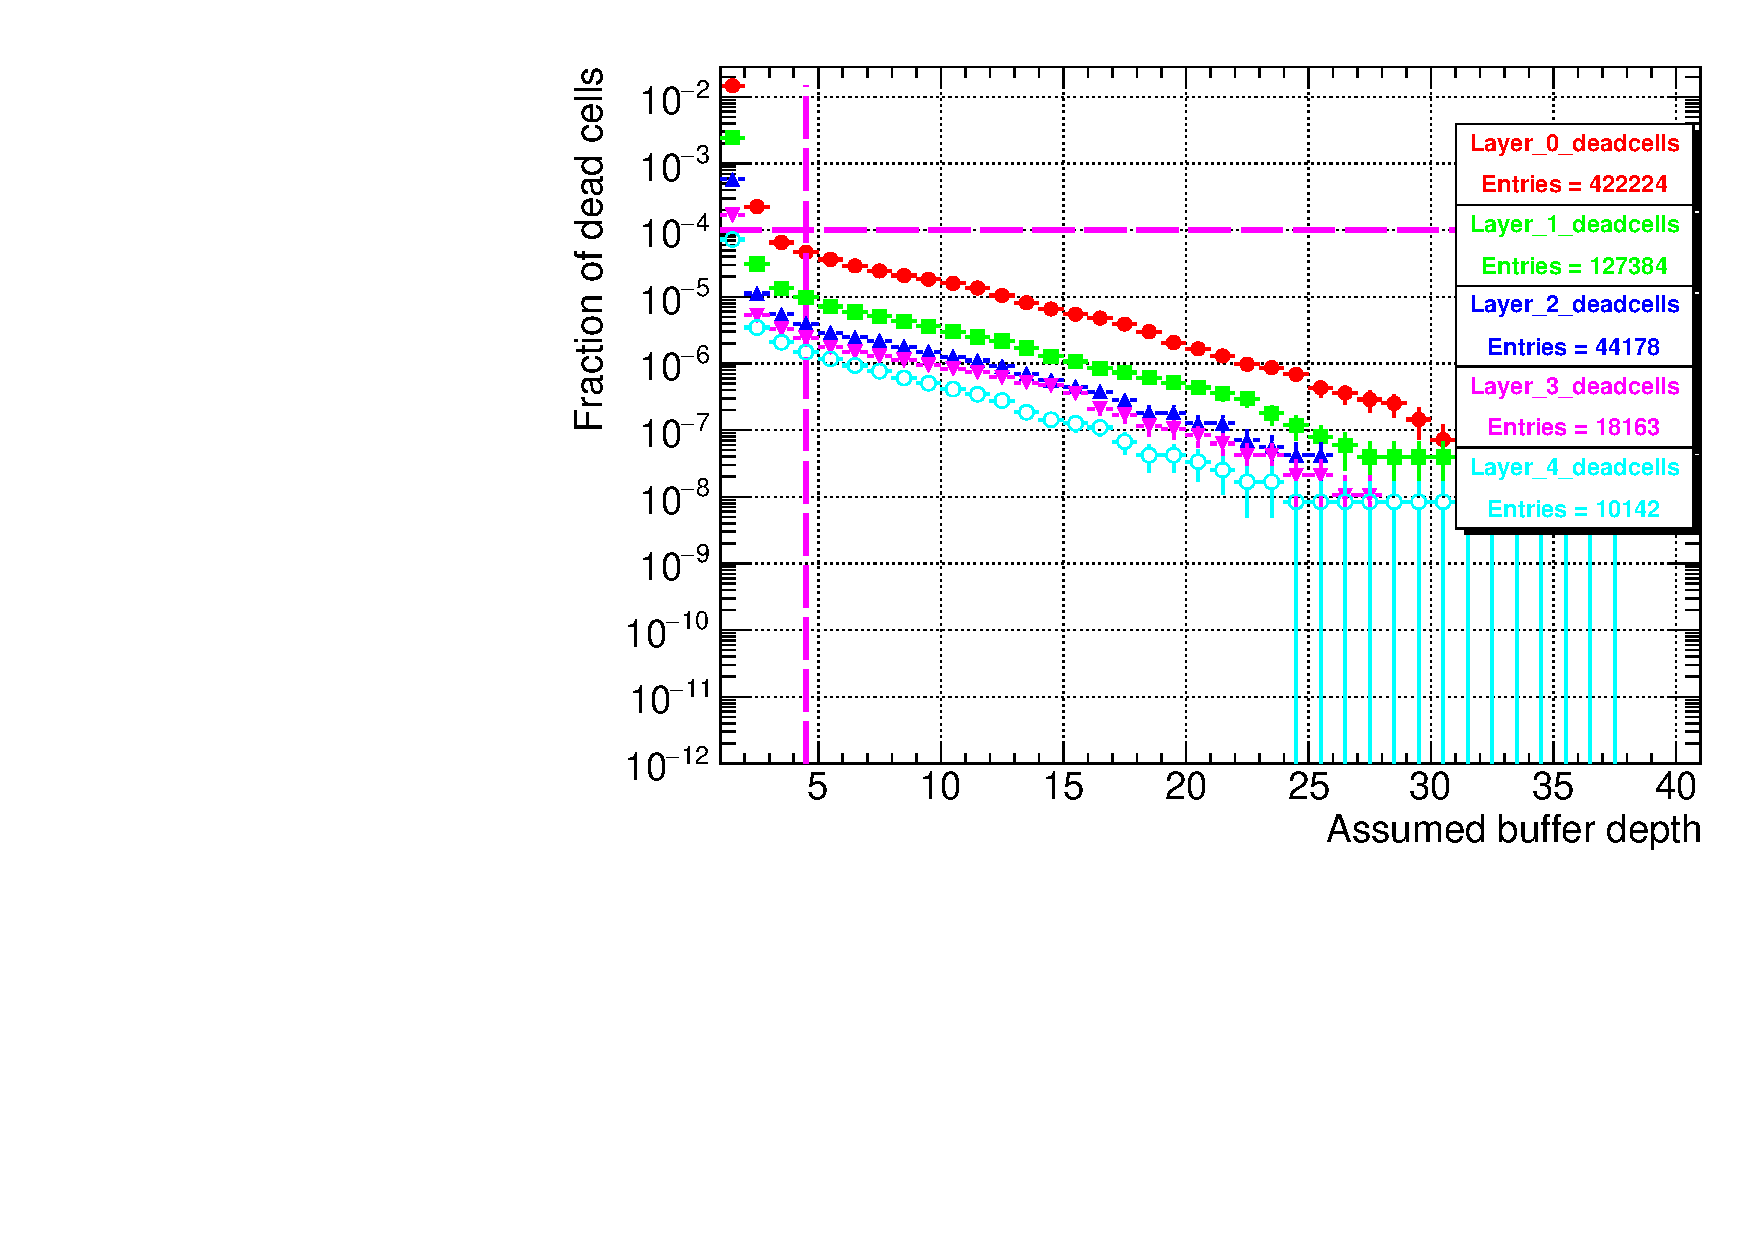
\includegraphics[width=\textwidth]{Figures/Pairs/Appendix/occupancy_deadcells_SiVertexBarrel_ILC250_TDR_corrected_Barrel_size.pdf}
   \caption{Set (TDR), fraction of dead cells}
   \end{subfigure}\\
  \begin{subfigure}[b]{0.49\textwidth}
   \centering
    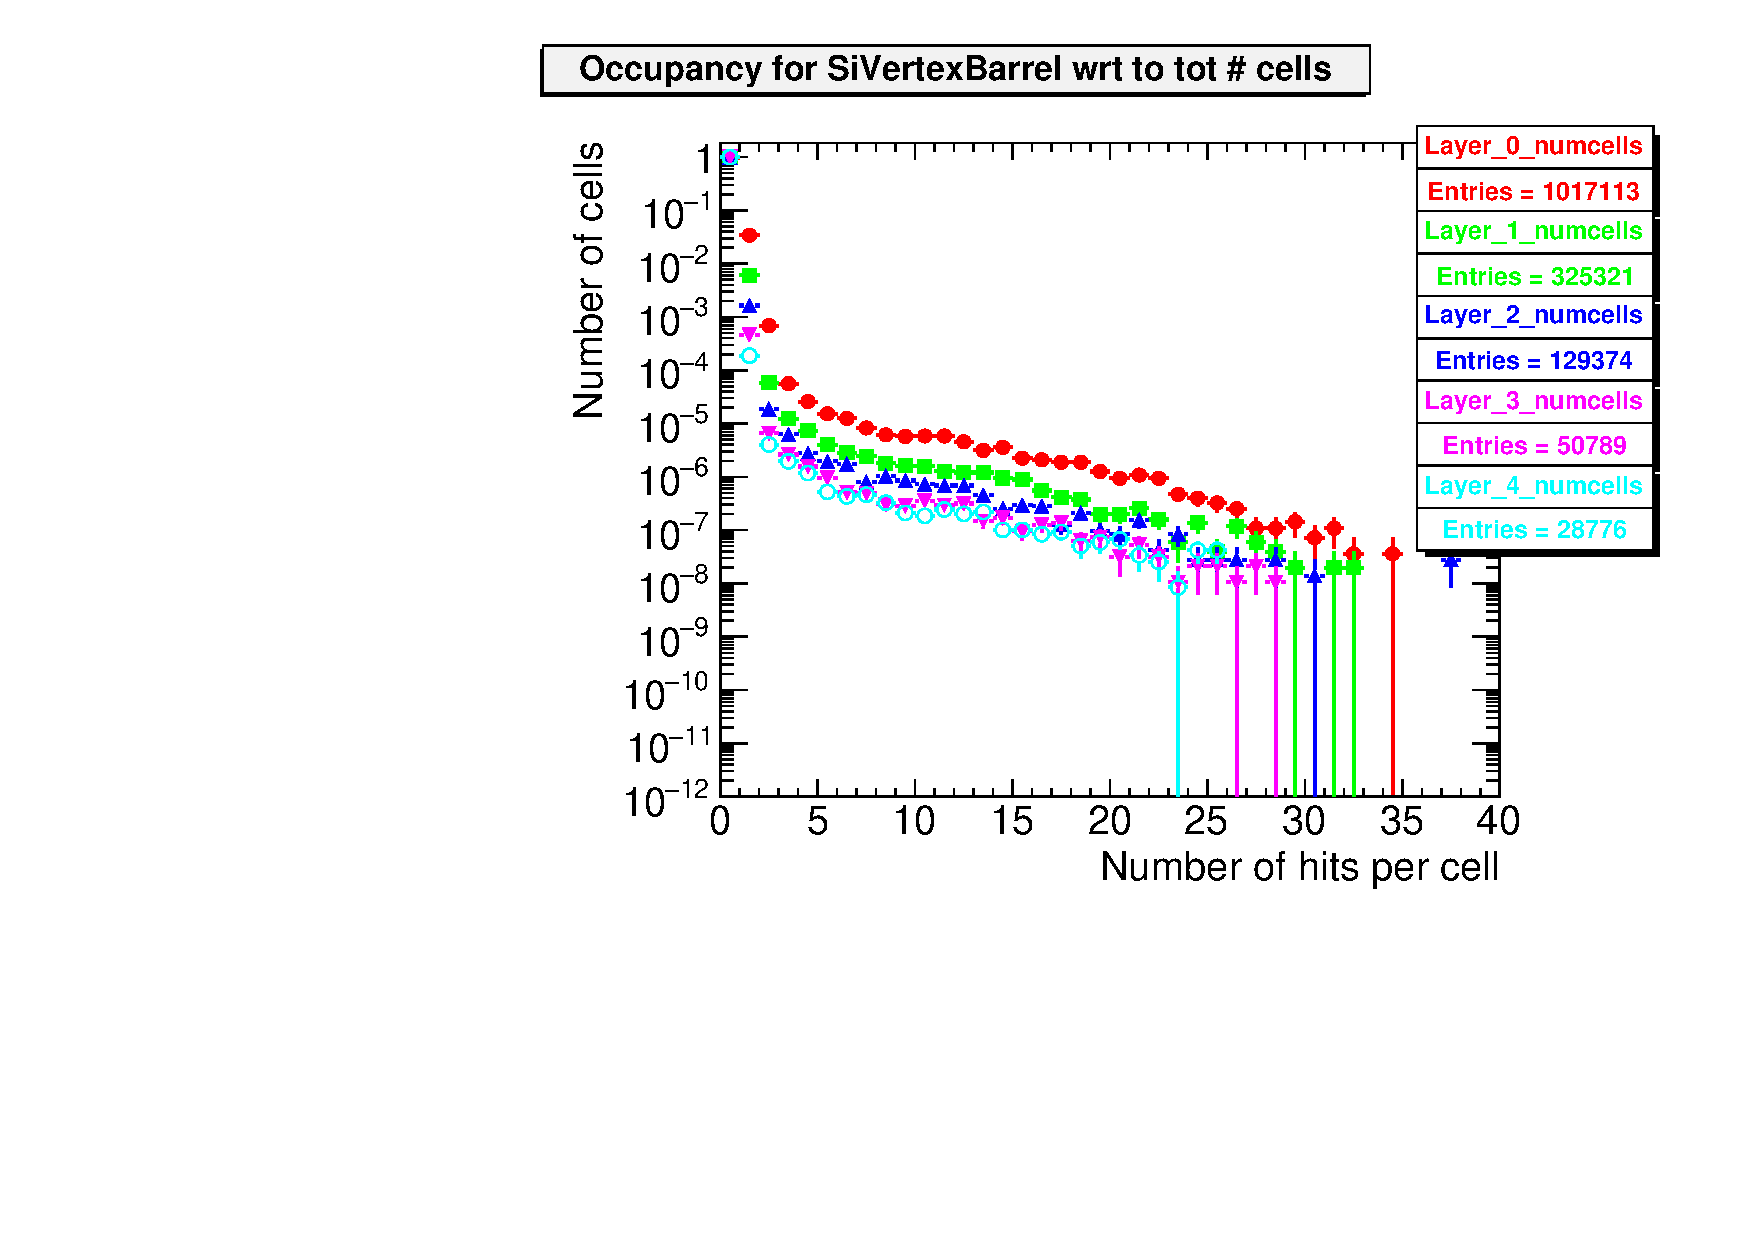
\includegraphics[width=\textwidth]{Figures/Pairs/Appendix/occupancy_numcells_SiVertexBarrel_ILC250_SetA_corrected_Barrel_size.pdf}
   \caption{Set (A), normalized occupancy}
   \end{subfigure}
   \hfill
    \begin{subfigure}[b]{0.49\textwidth}
   \centering
    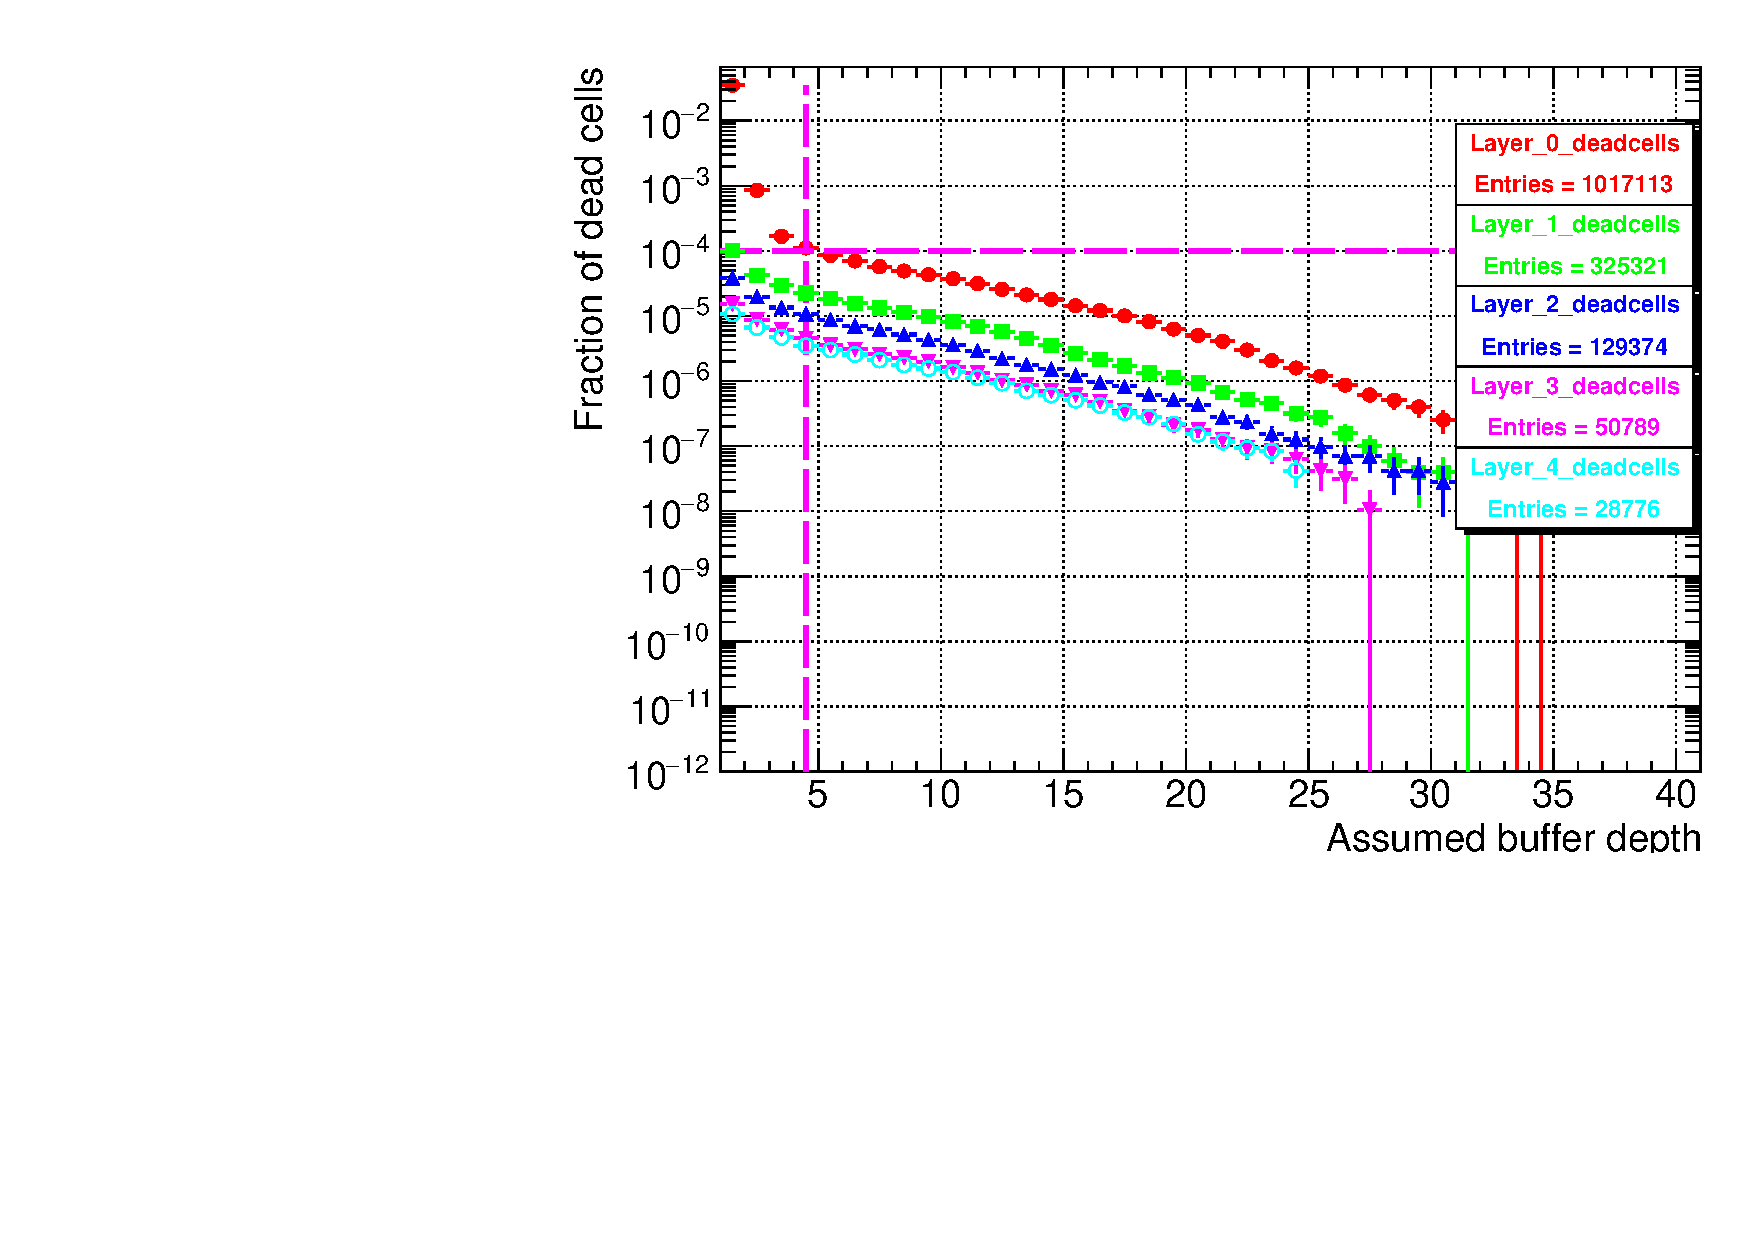
\includegraphics[width=\textwidth]{Figures/Pairs/Appendix/occupancy_deadcells_SiVertexBarrel_ILC250_SetA_corrected_Barrel_size.pdf}
   \caption{Set (A), fraction of dead cells}
   \end{subfigure}
      \caption[Pair background occupancy in all SiD vertex detector barrel layers for the ILC250]{ILC250 pair background occupancy in all SiD vertex detector barrel layers, after a full bunch train (1312 bunch crossings).
   The left hand figures show the occupancy in the individual vertex detector layer, normalized by the total number of cells of the corresponding layer.
   The right hand figures show the fraction of the dead cells in the individual vertex detector layer, with respect to the total number of cells.
   \\The dashed lines indicate the the buffer depth of four for the current sensor design, and the guideline of \num{e-4} for a critical acceptance limit.
   }
   \label{fig:PairBkg:ILC250_Occupancy_Layers_VXDBarrel}
     \end{figure}
  \begin{figure}[htb]\ContinuedFloat
     \begin{subfigure}[b]{0.49\textwidth}
   \centering
    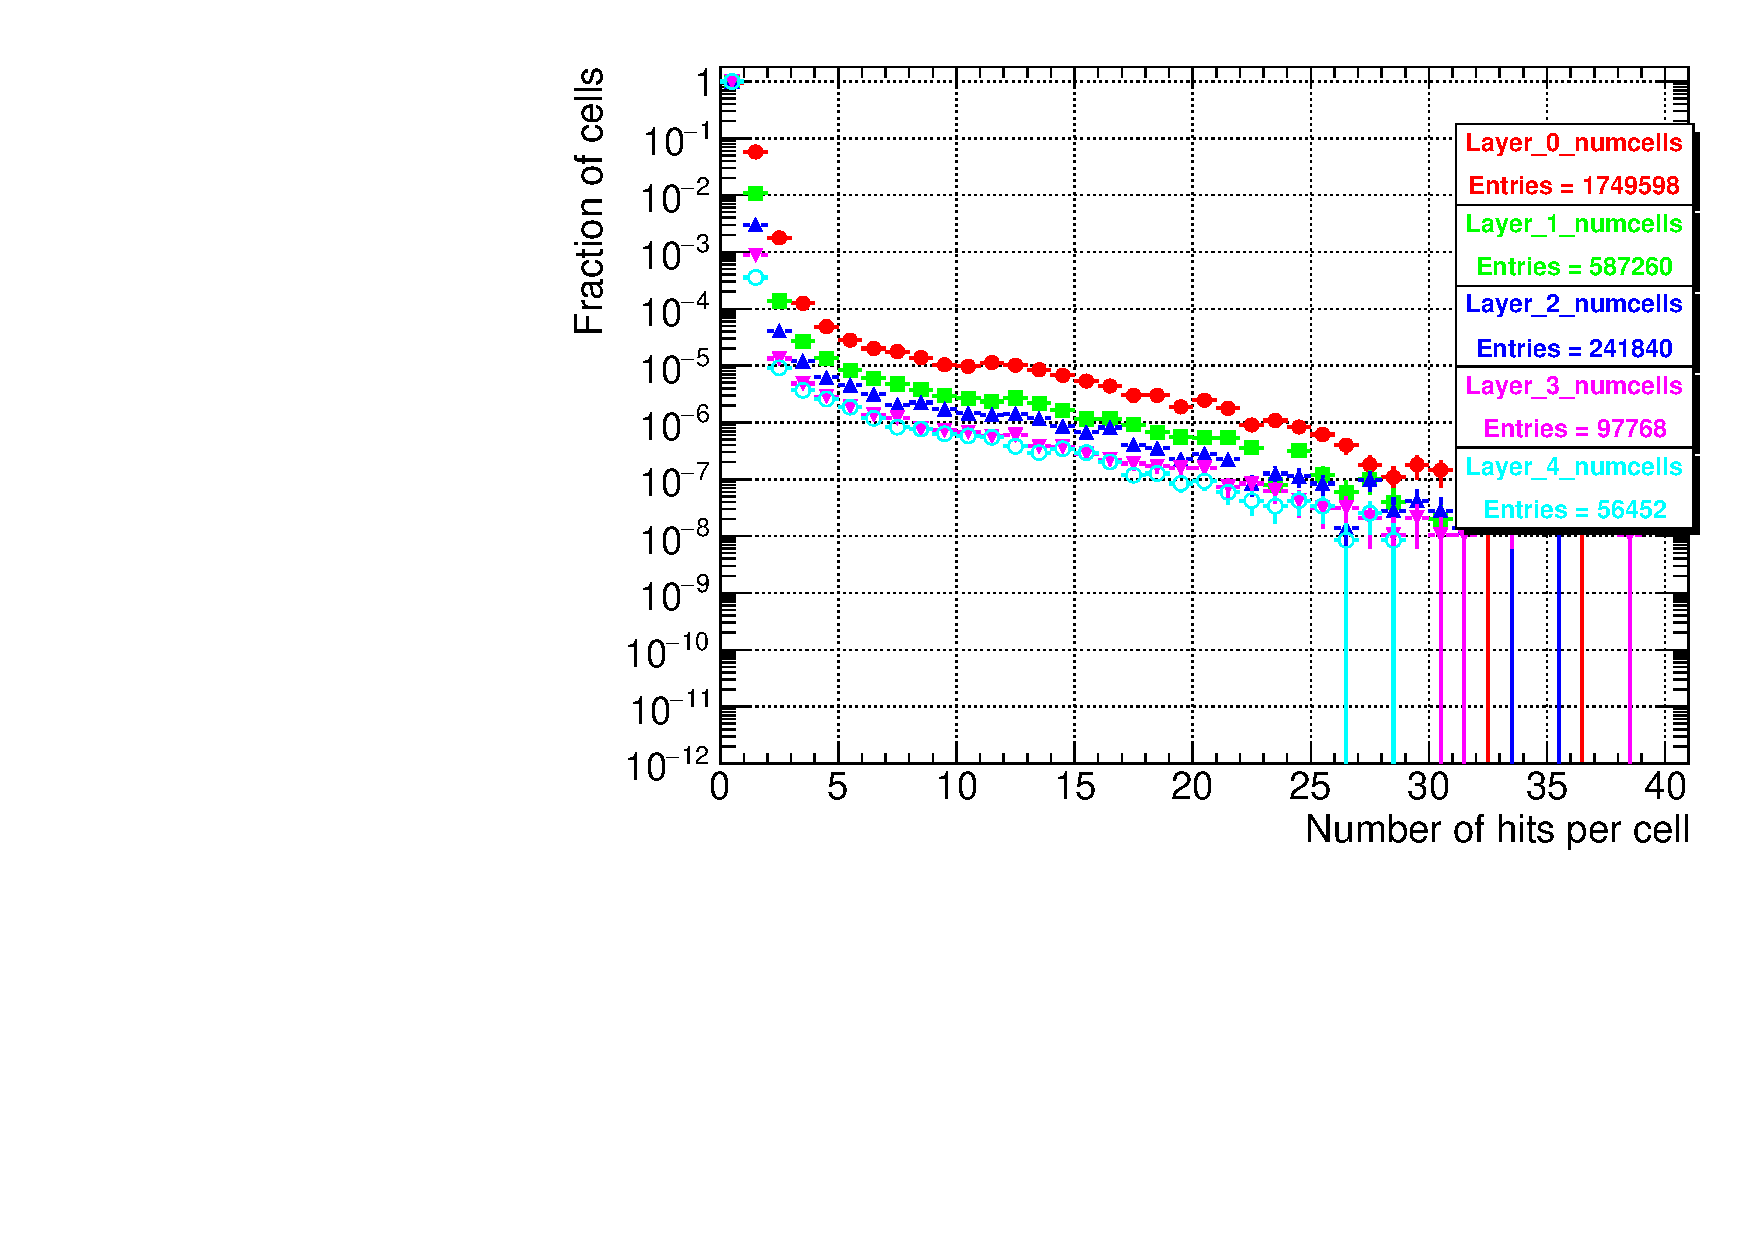
\includegraphics[width=\textwidth]{Figures/Pairs/Appendix/occupancy_numcells_SiVertexBarrel_ILC250_SetB_corrected_Barrel_size.pdf}
   \caption{Set (B), normalized occupancy}
   \end{subfigure}
   \hfill
    \begin{subfigure}[b]{0.49\textwidth}
   \centering
    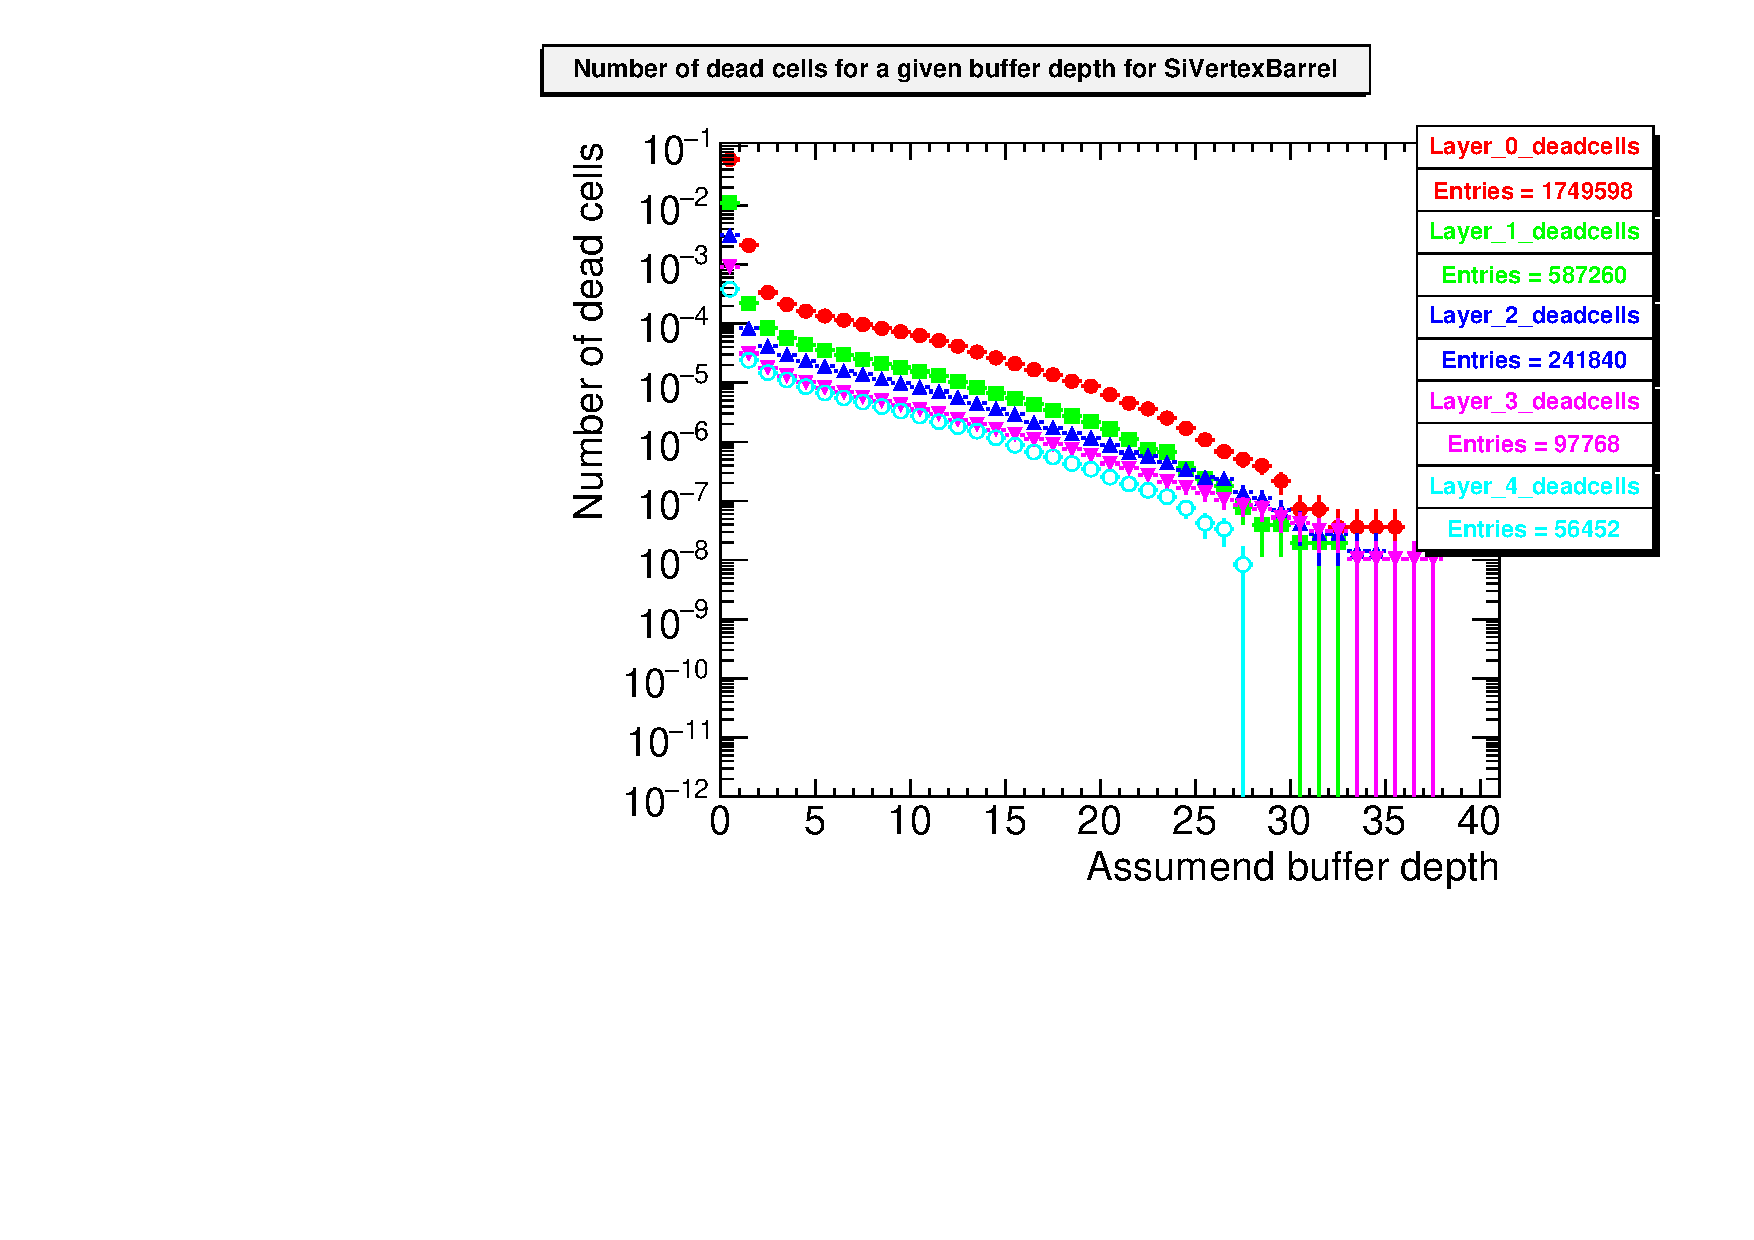
\includegraphics[width=\textwidth]{Figures/Pairs/Appendix/occupancy_deadcells_SiVertexBarrel_ILC250_SetB_corrected_Barrel_size.pdf}
    \caption{Set (B), fraction of dead cells}
   \end{subfigure}\\
     \begin{subfigure}[b]{0.49\textwidth}
   \centering
    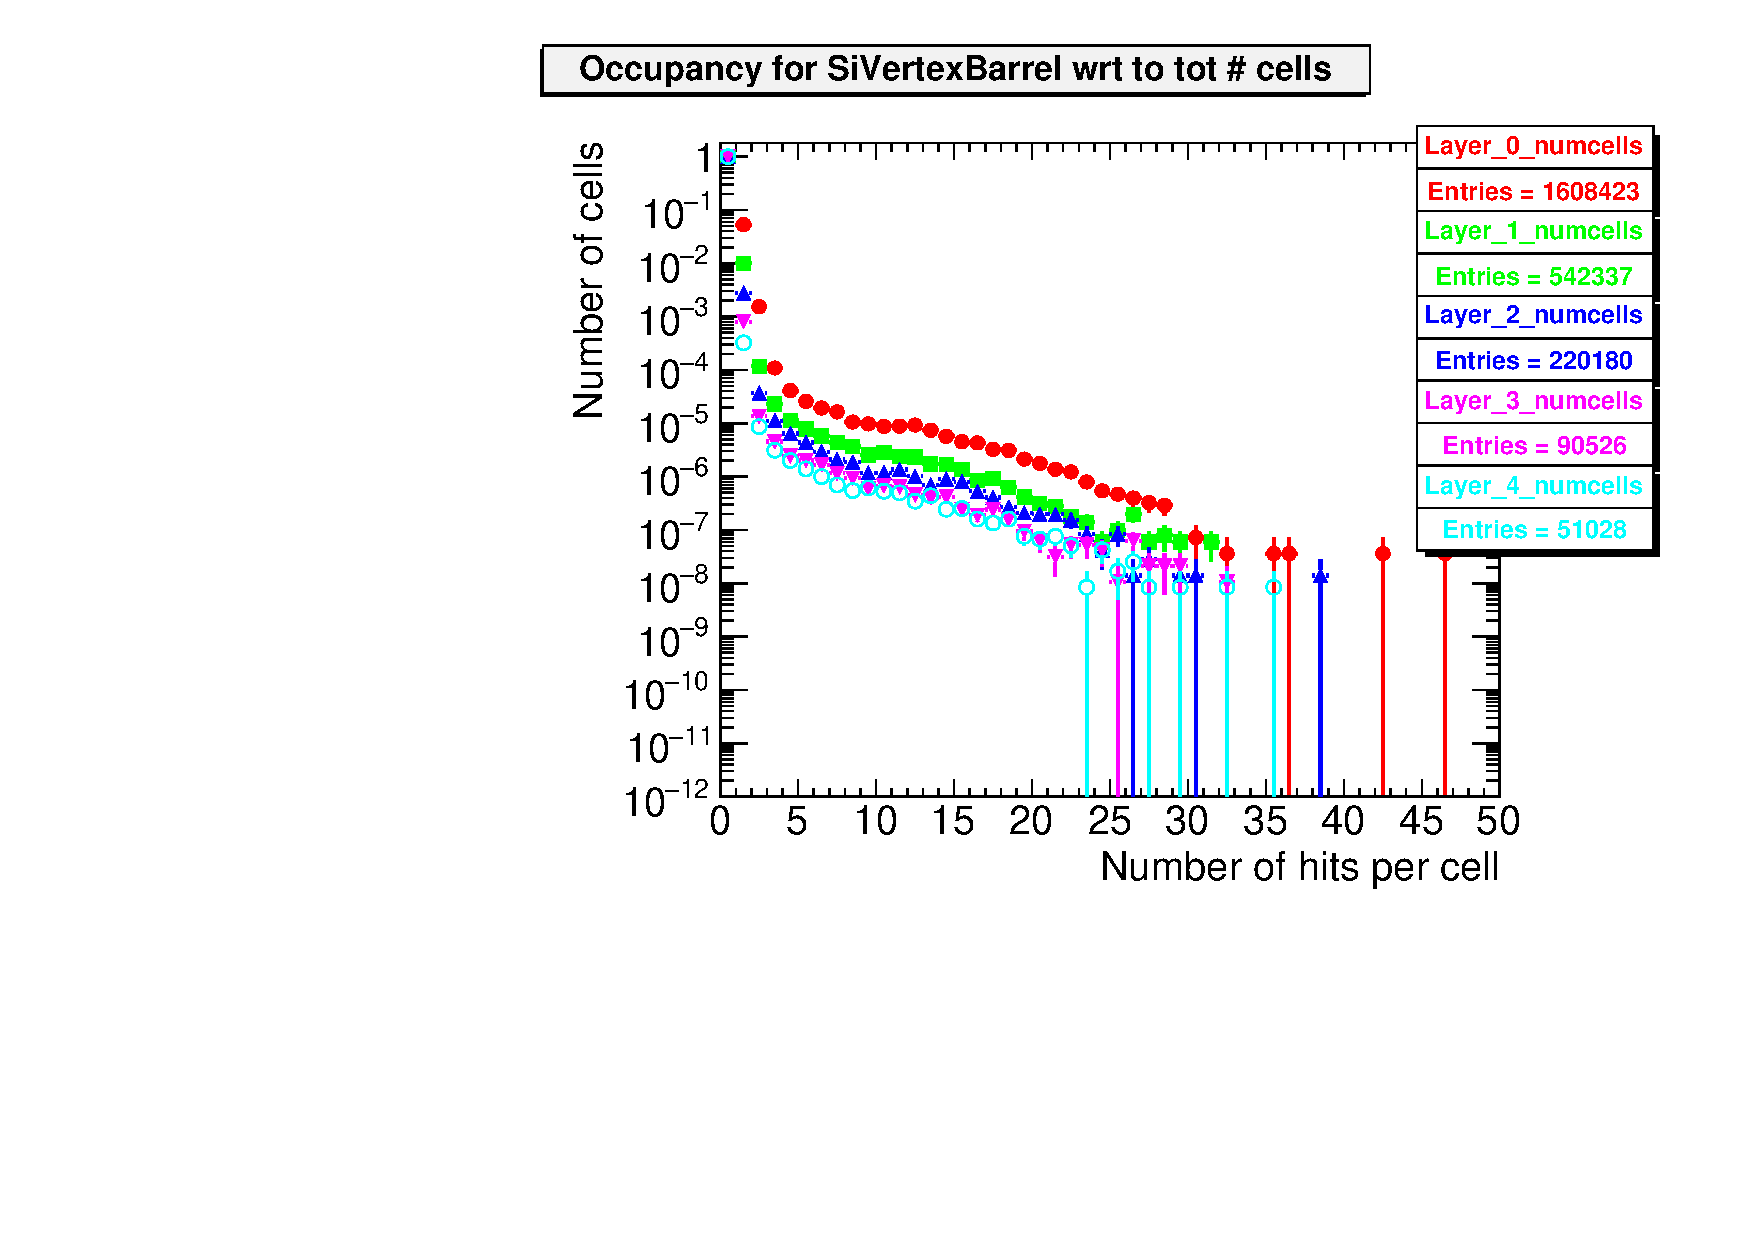
\includegraphics[width=\textwidth]{Figures/Pairs/Appendix/occupancy_numcells_SiVertexBarrel_ILC250_SetC_corrected_Barrel_size.pdf}
   \caption{Set (C), normalized occupancy}
   \end{subfigure}
   \hfill
    \begin{subfigure}[b]{0.49\textwidth}
   \centering
   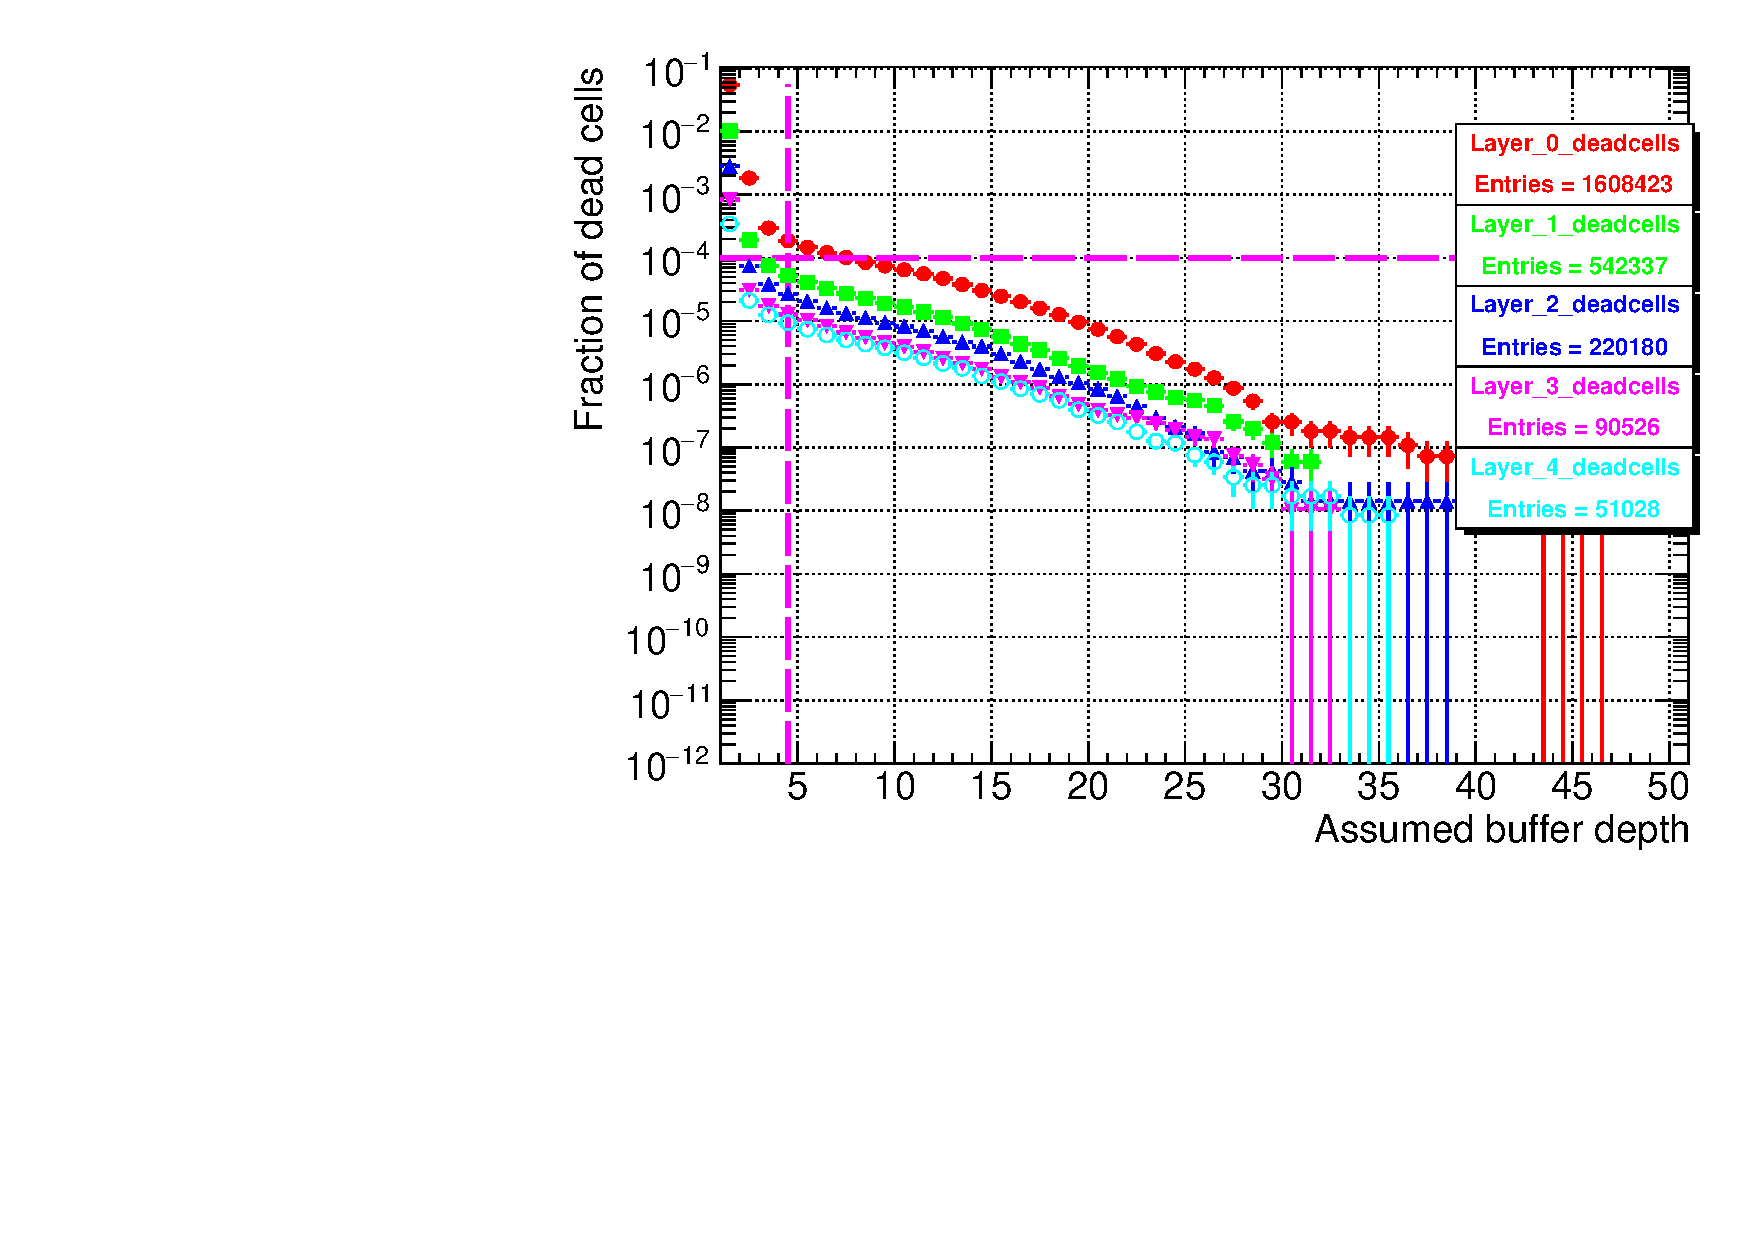
\includegraphics[width=\textwidth]{Figures/Pairs/Appendix/occupancy_deadcells_SiVertexBarrel_ILC250_SetC_corrected_Barrel_size.pdf}
   \caption{Set (C), fraction of dead cells}
   \end{subfigure}
   \caption[Pair background occupancy in all SiD vertex detector barrel layers for the ILC250]{ILC250 pair background occupancy in all SiD vertex detector barrel layers, after a full bunch train (1312 bunch crossings).
   The left hand figures show the occupancy in the individual vertex detector layer, normalized by the total number of cells of the corresponding layer.
   The right hand figures show the fraction of the dead cells in the individual vertex detector layer, with respect to the total number of cells.
   \\The dashed lines indicate the the buffer depth of four for the current sensor design, and the guideline of \num{e-4} for a critical acceptance limit.
   }
   %\label{fig:PairBkg:ILC250_Occupancy_Layers_VXDBarrel}
 \end{figure}

   \begin{figure}[!htbp]
 \centering
   \begin{subfigure}[b]{0.49\textwidth}
   \centering
    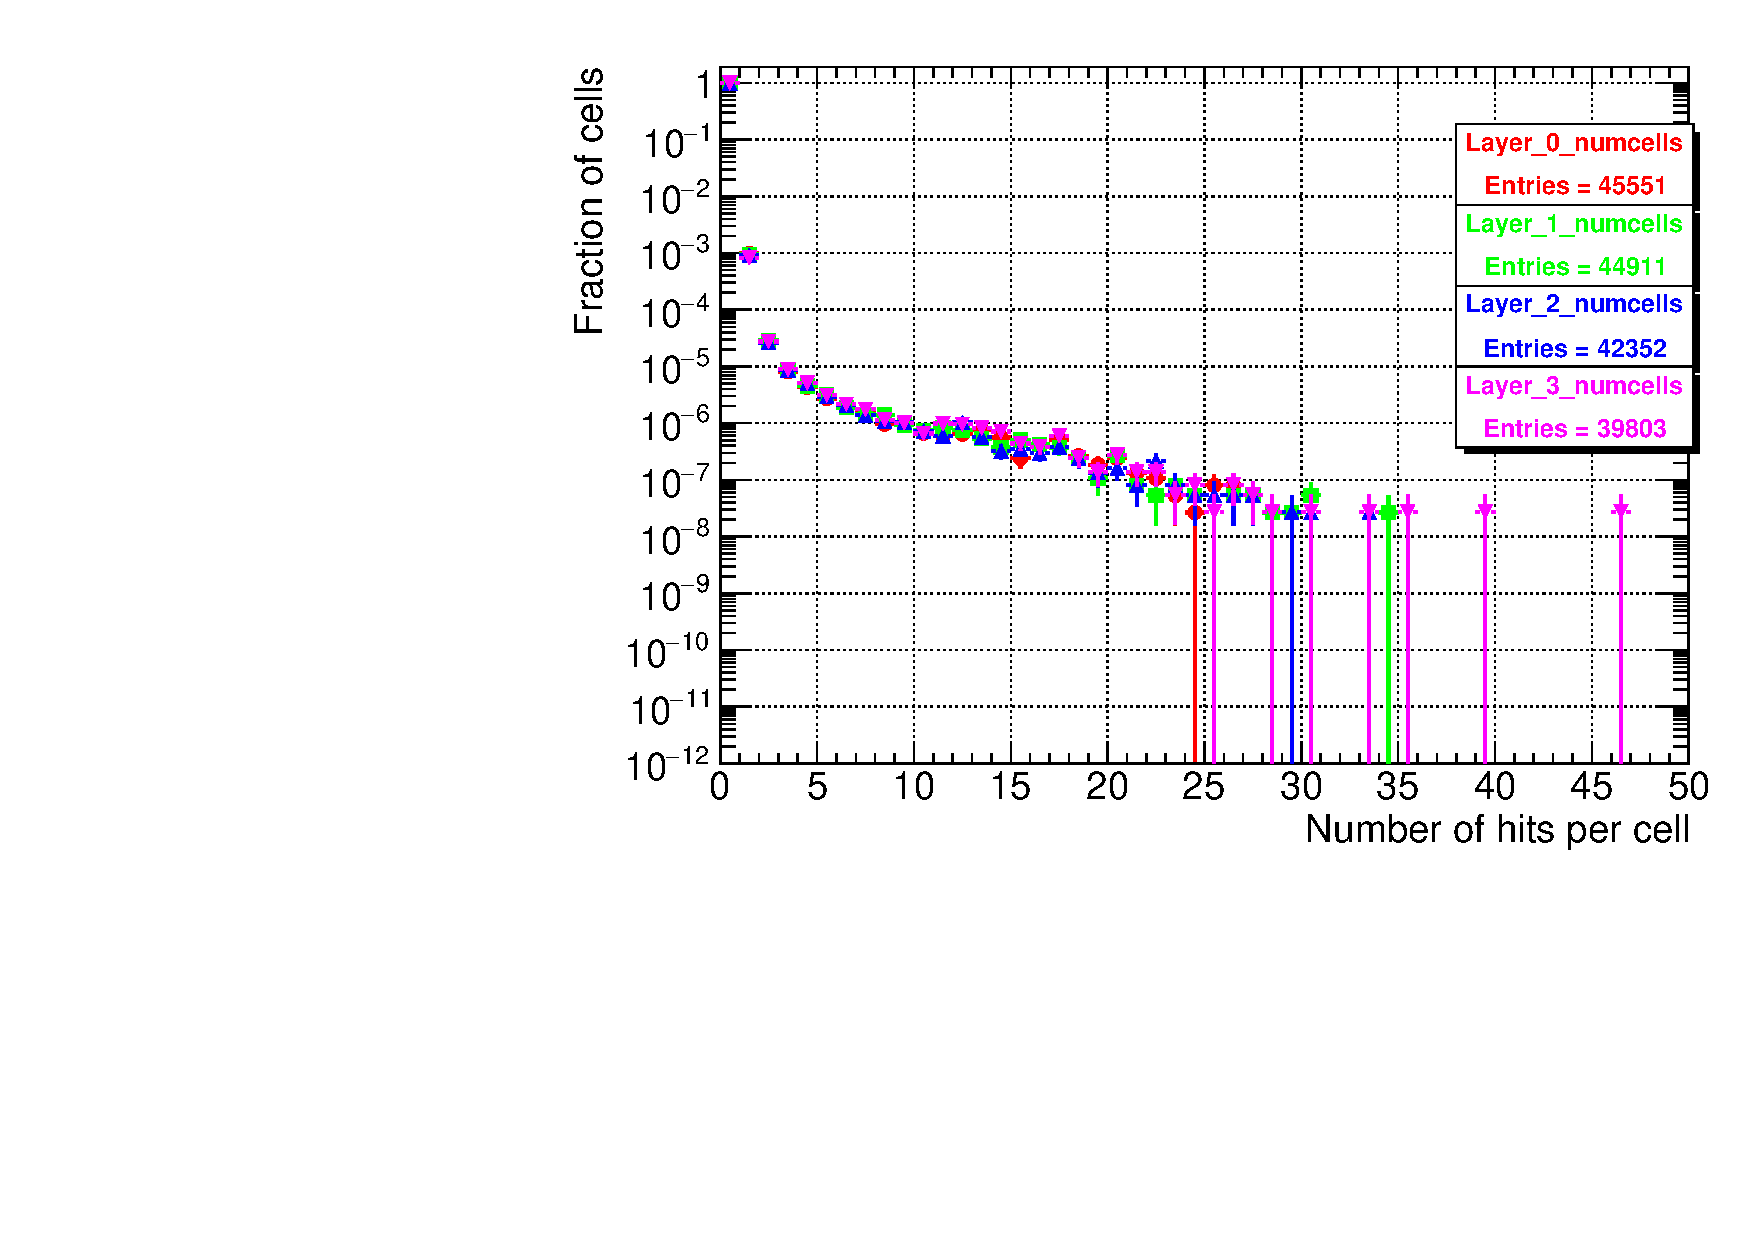
\includegraphics[width=\textwidth]{Figures/Pairs/Appendix/occupancy_numcells_SiVertexEndcap_ILC250_TDR.pdf}
   \caption{Set (TDR), normalized occupancy}
   \end{subfigure}
   \hfill
    \begin{subfigure}[b]{0.49\textwidth}
   \centering
    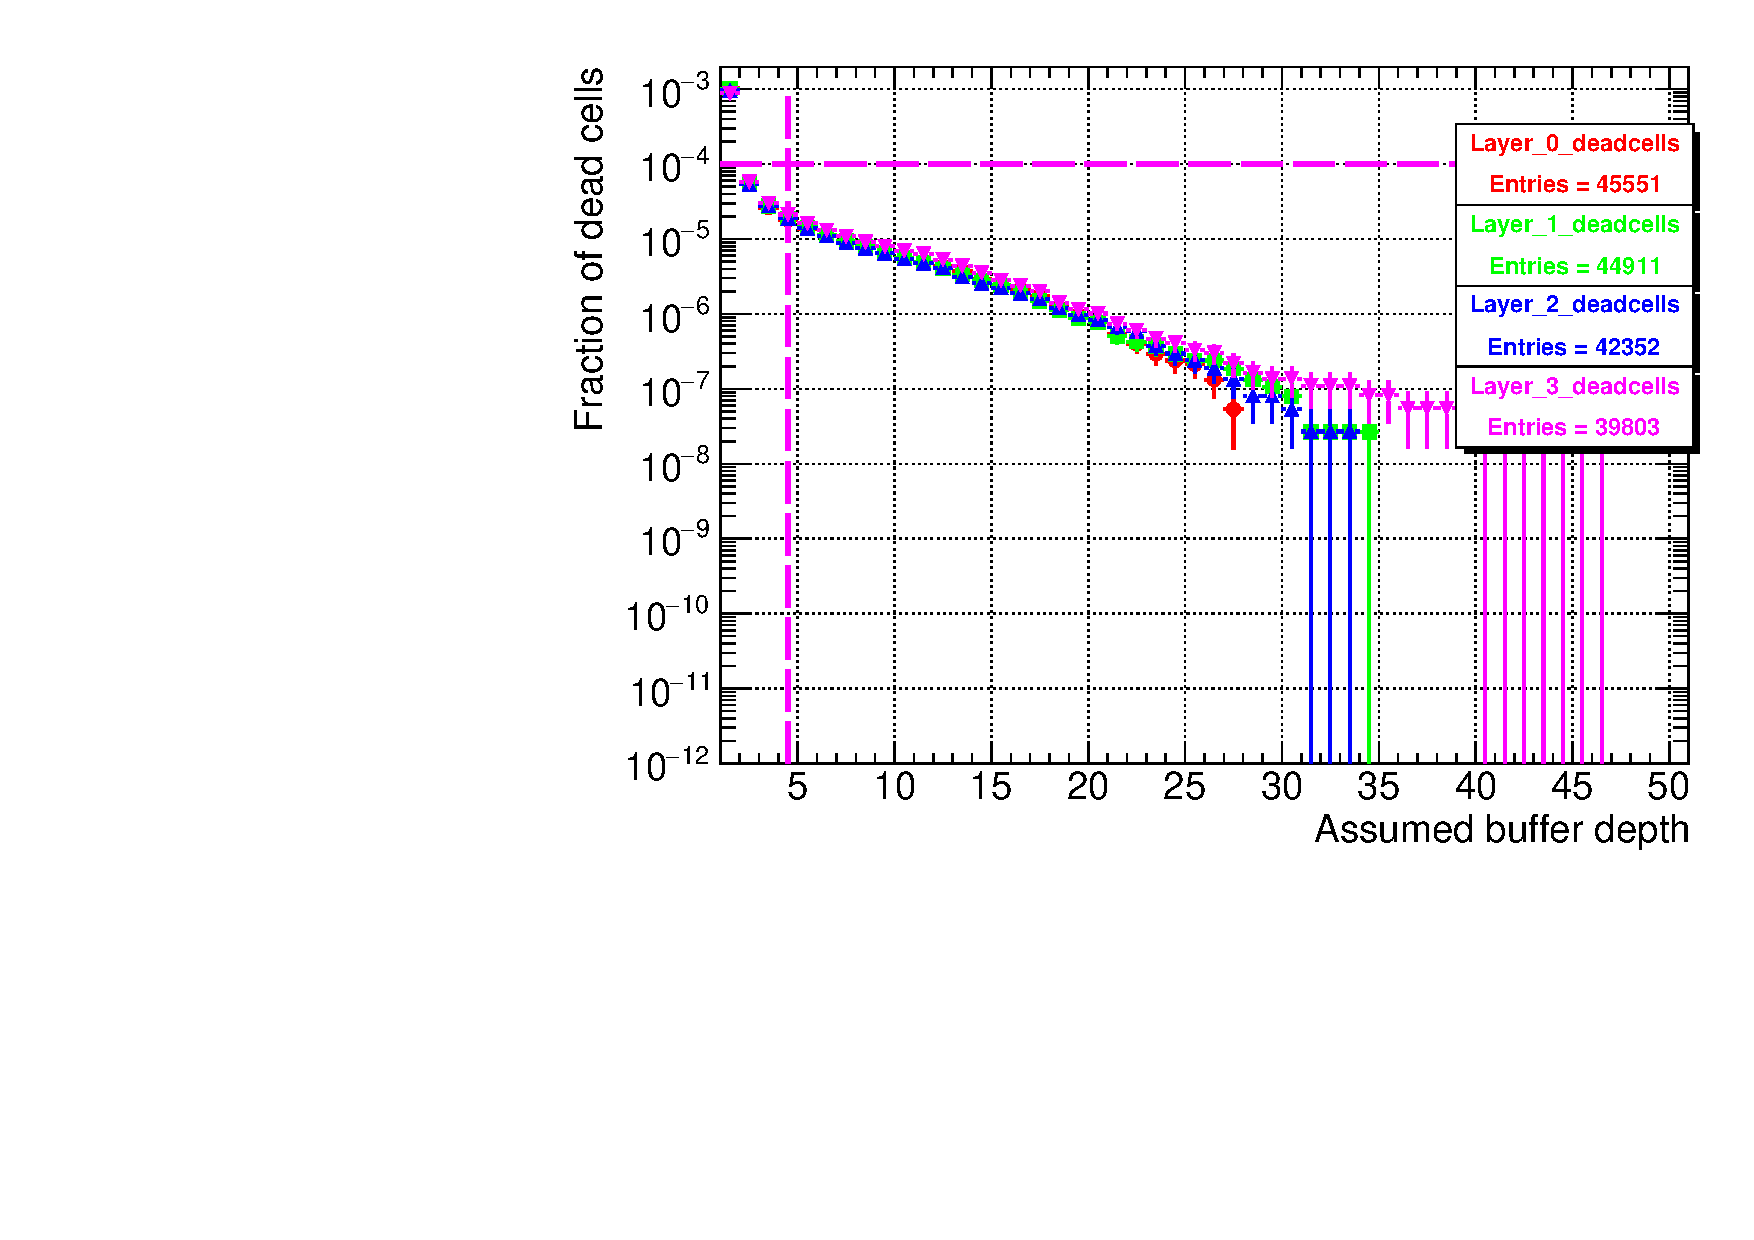
\includegraphics[width=\textwidth]{Figures/Pairs/Appendix/occupancy_deadcells_SiVertexEndcap_ILC250_TDR.pdf}
   \caption{Set (TDR), fraction of dead cells}
   \end{subfigure}\\
  \begin{subfigure}[b]{0.49\textwidth}
   \centering
    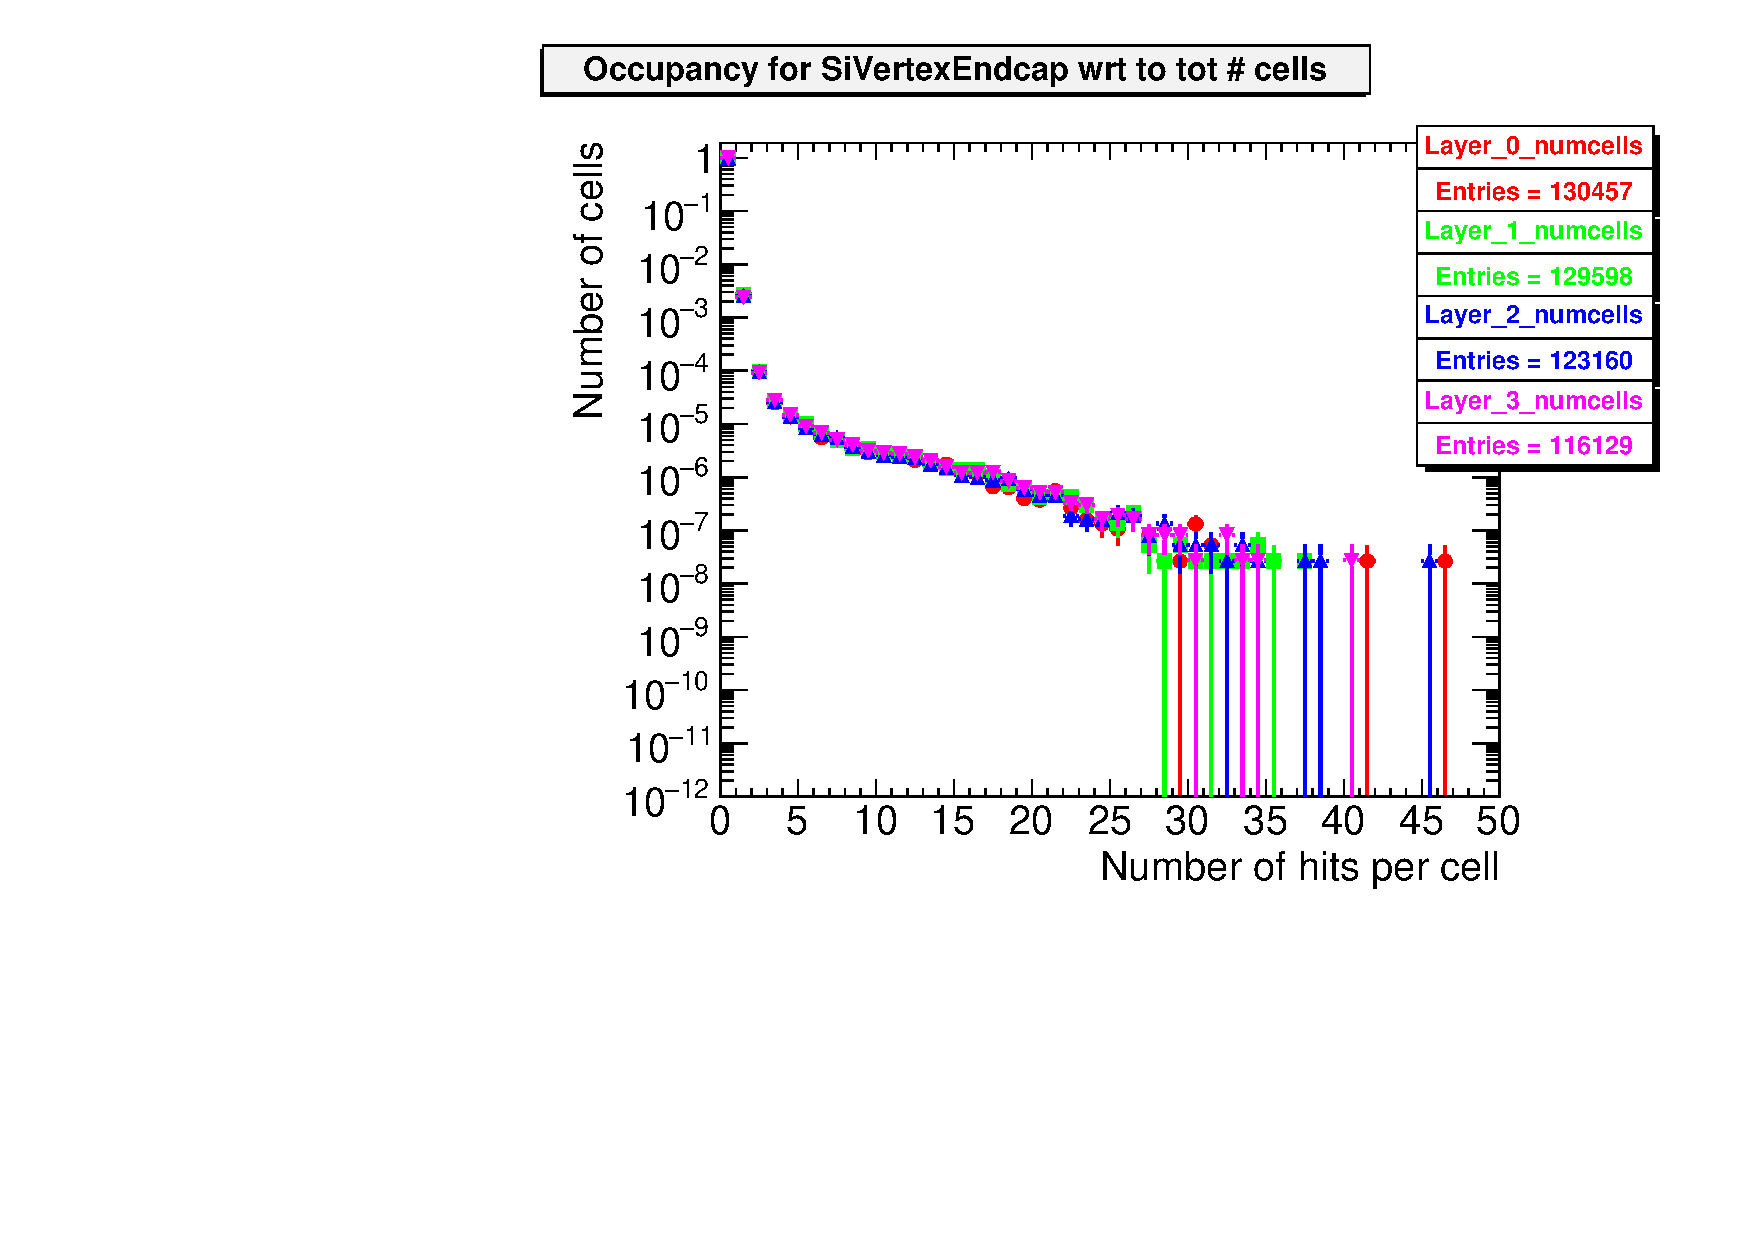
\includegraphics[width=\textwidth]{Figures/Pairs/Appendix/occupancy_numcells_SiVertexEndcap_ILC250_SetA.pdf}
   \caption{Set (A), normalized occupancy}
   \end{subfigure}
   \hfill
    \begin{subfigure}[b]{0.49\textwidth}
   \centering
    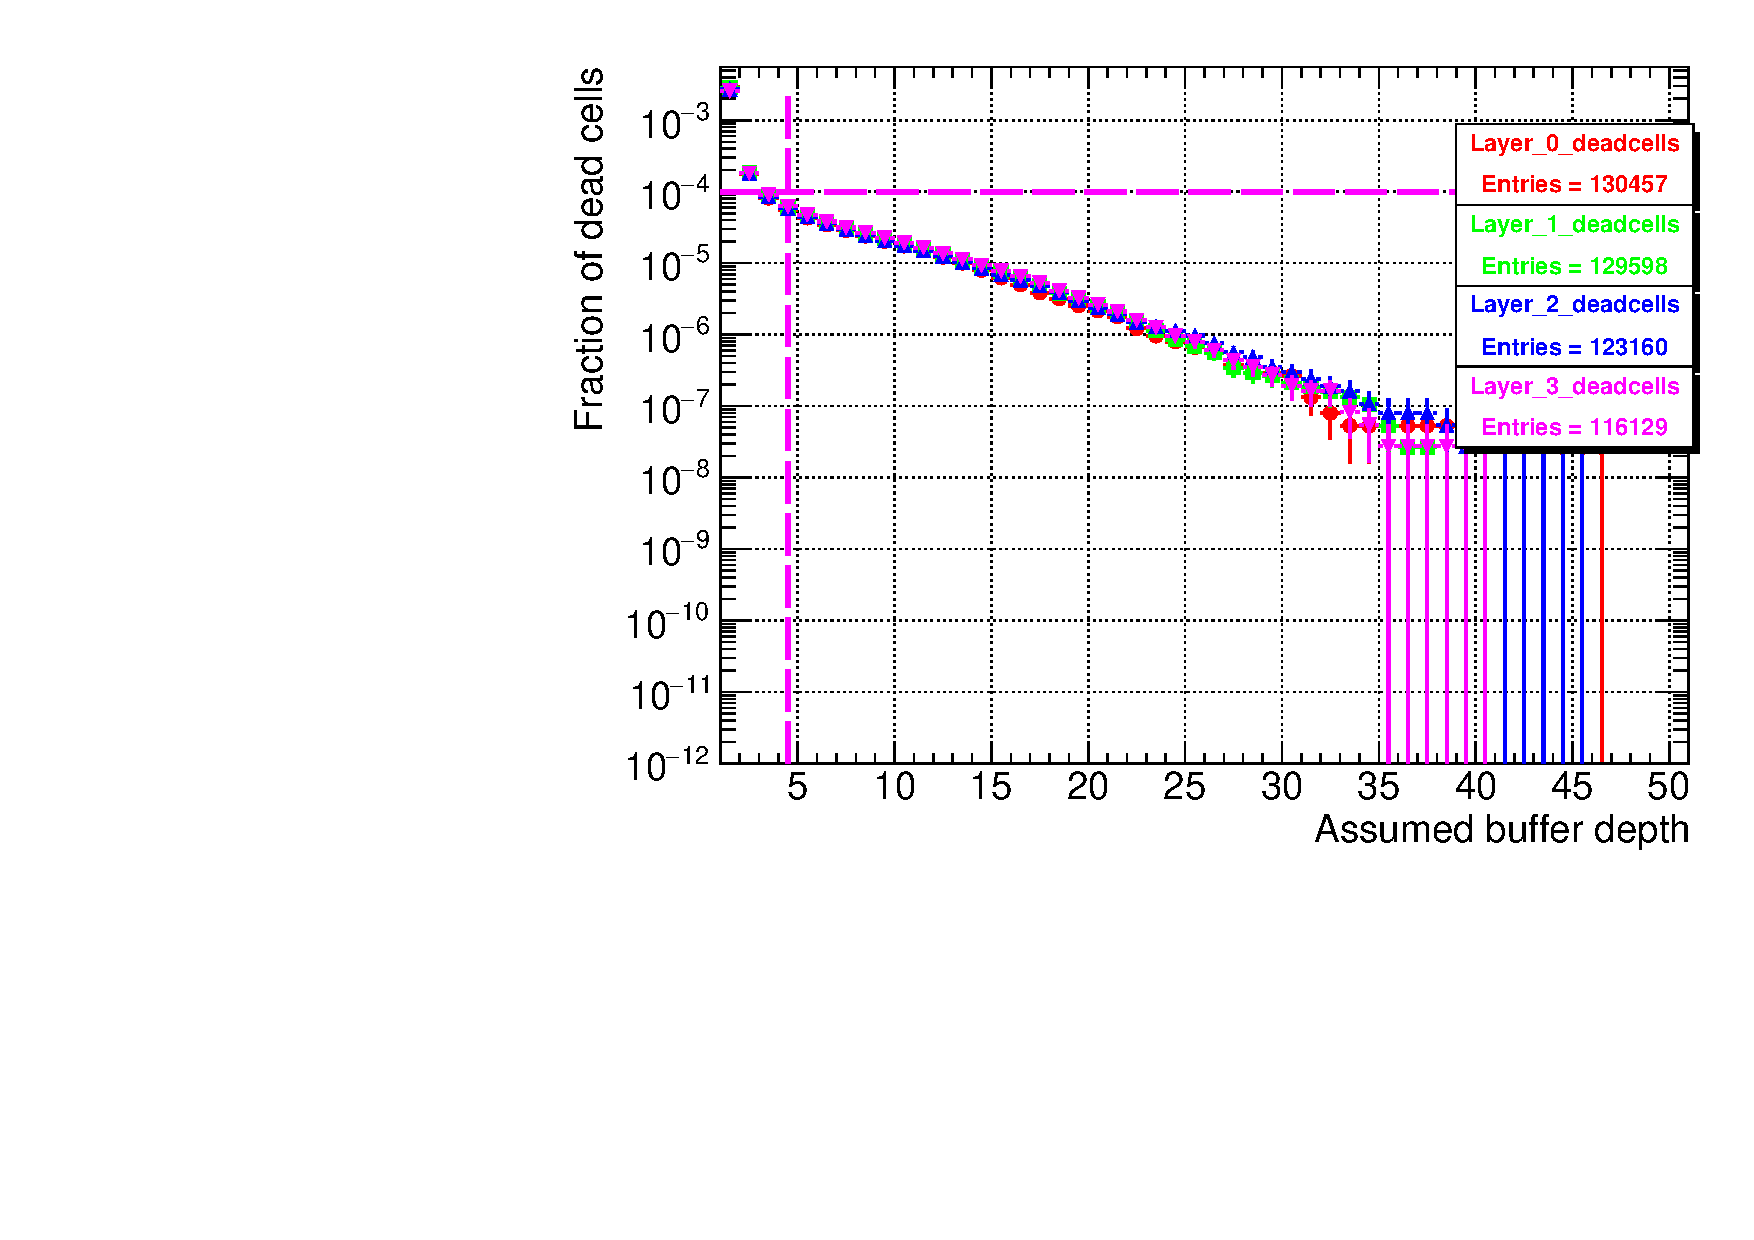
\includegraphics[width=\textwidth]{Figures/Pairs/Appendix/occupancy_deadcells_SiVertexEndcap_ILC250_SetA.pdf}
   \caption{Set (A), fraction of dead cells}
   \end{subfigure}
      \caption[Pair background occupancy in all SiD vertex detector endcap layers for the ILC250]{ILC250 pair background occupancy in all SiD vertex detector endcap layers, after a full bunch train (1312 bunch crossings).
   The left hand figures show the occupancy in the individual vertex detector layer, normalized by the total number of cells of the corresponding layer.
   The right hand figures show the fraction of the dead cells in the individual vertex detector layer, with respect to the total number of cells.
   \\The dashed lines indicate the the buffer depth of four for the current sensor design, and the guideline of \num{e-4} for a critical acceptance limit.
   }
   \label{fig:PairBkg:ILC250_Occupancy_Layers_VXDEndcap}
  \end{figure}
  \begin{figure}[htb]\ContinuedFloat
     \begin{subfigure}[b]{0.49\textwidth}
   \centering
    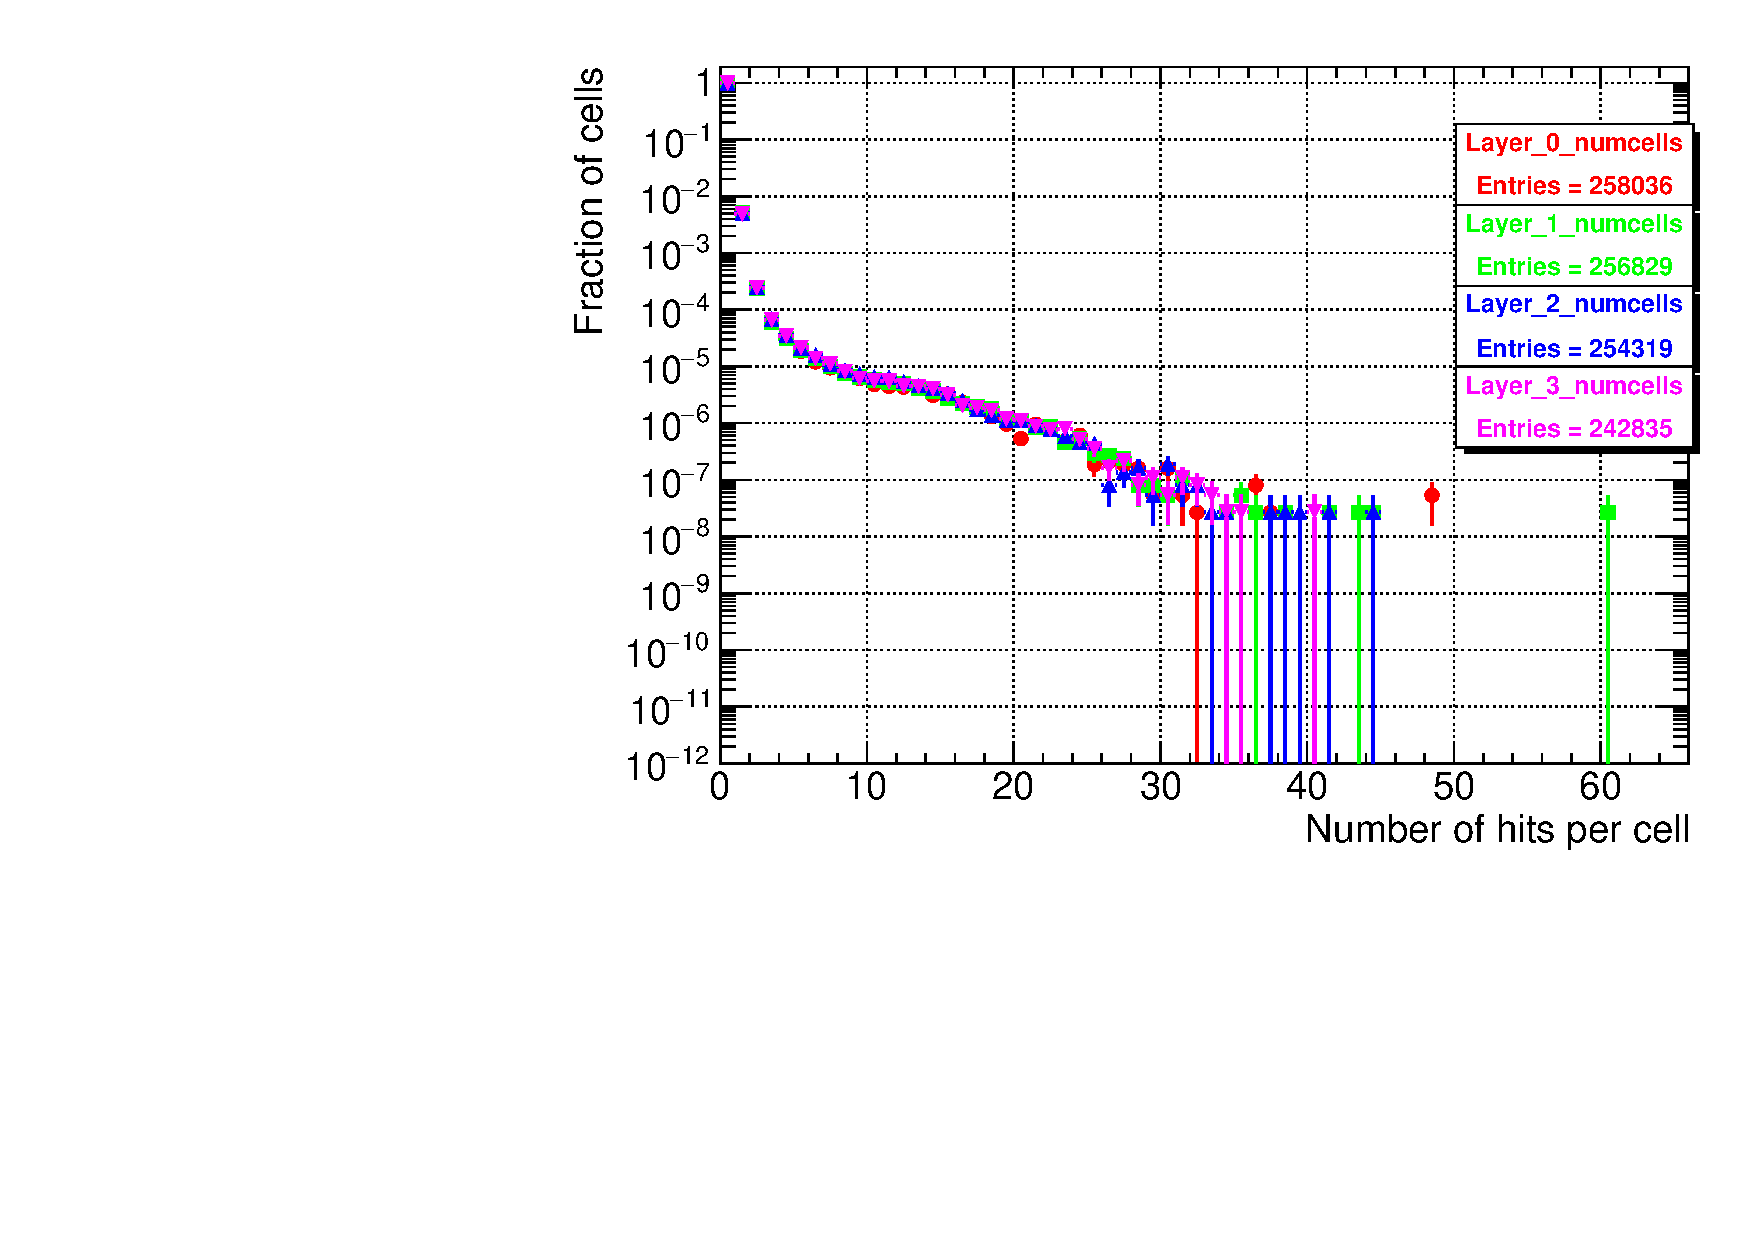
\includegraphics[width=\textwidth]{Figures/Pairs/Appendix/occupancy_numcells_SiVertexEndcap_ILC250_SetB.pdf}
   \caption{Set (B), normalized occupancy}
   \end{subfigure}
   \hfill
    \begin{subfigure}[b]{0.49\textwidth}
   \centering
    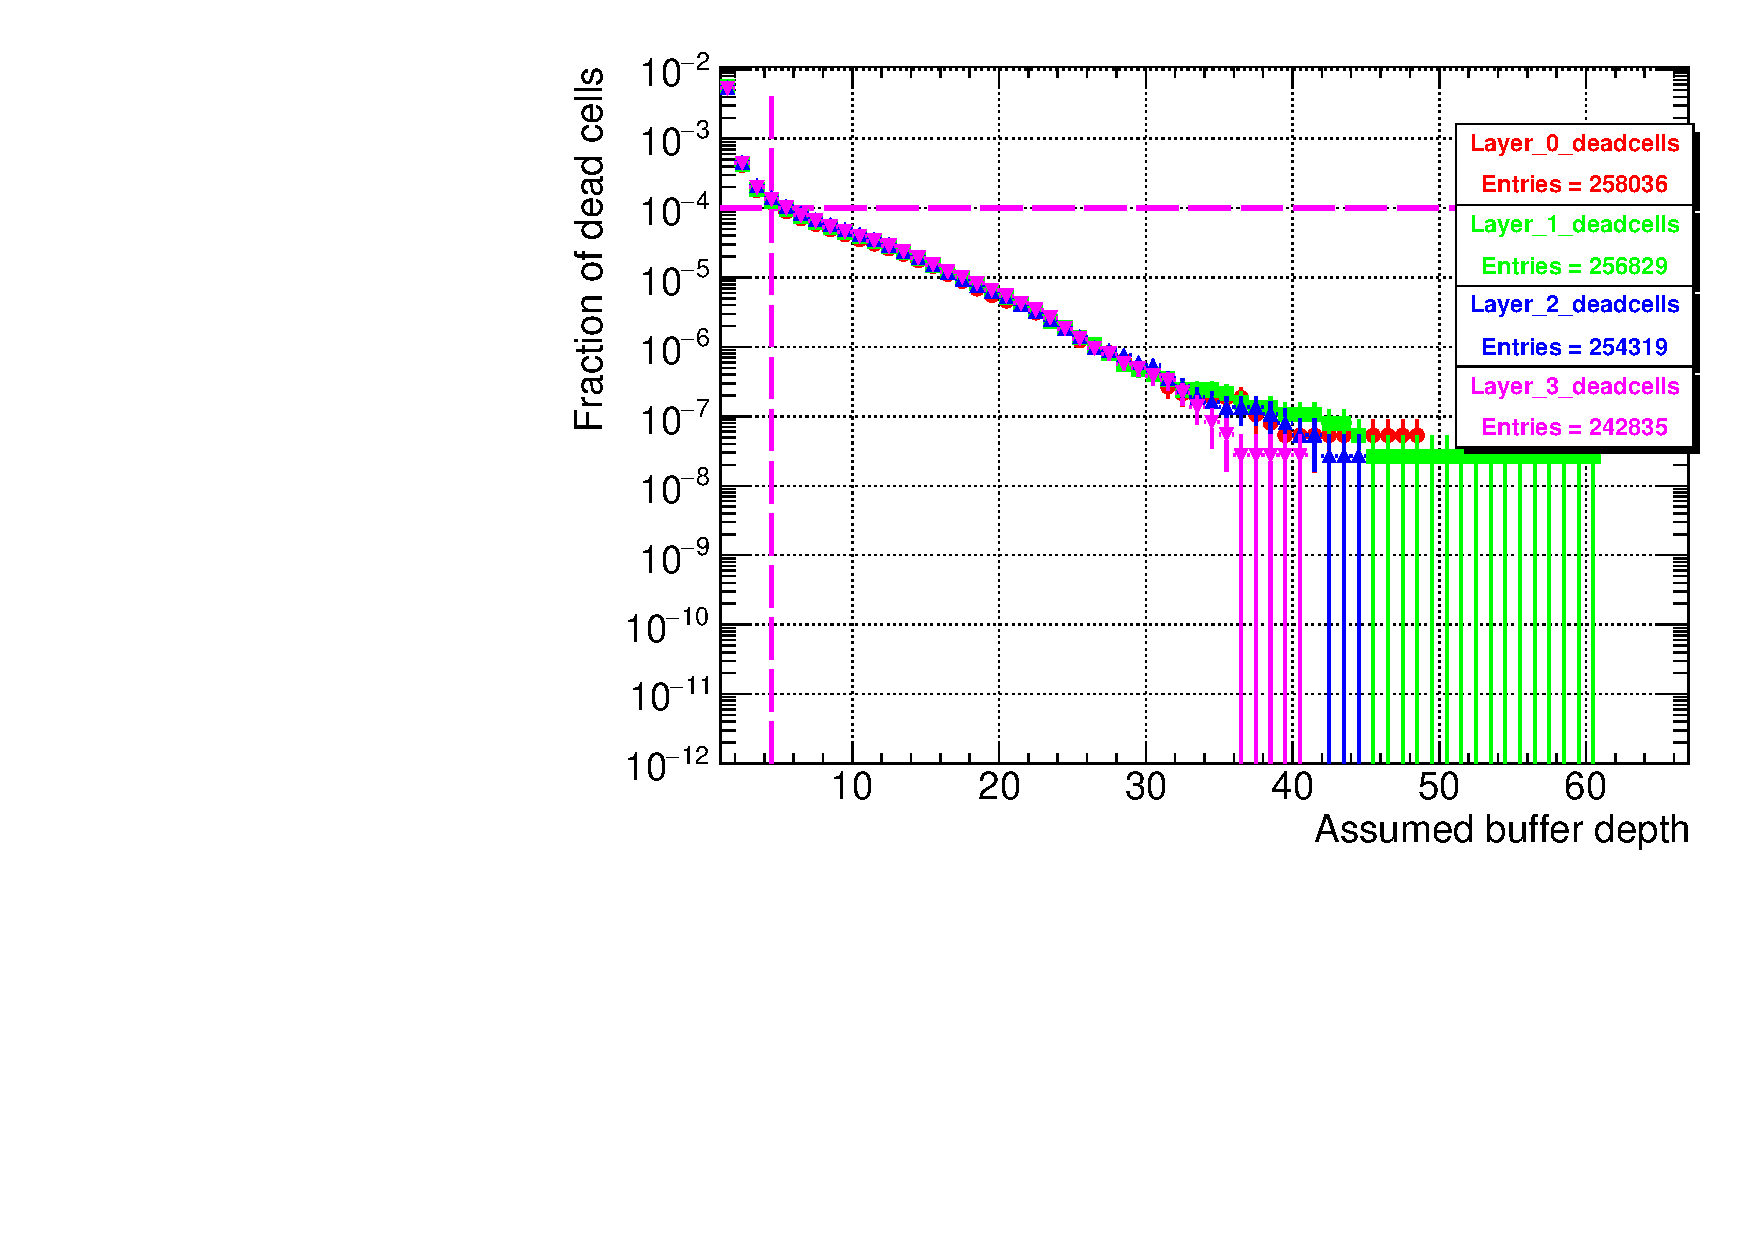
\includegraphics[width=\textwidth]{Figures/Pairs/Appendix/occupancy_deadcells_SiVertexEndcap_ILC250_SetB.pdf}
   \caption{Set (B), fraction of dead cells}
   \end{subfigure}\\
     \begin{subfigure}[b]{0.49\textwidth}
   \centering
    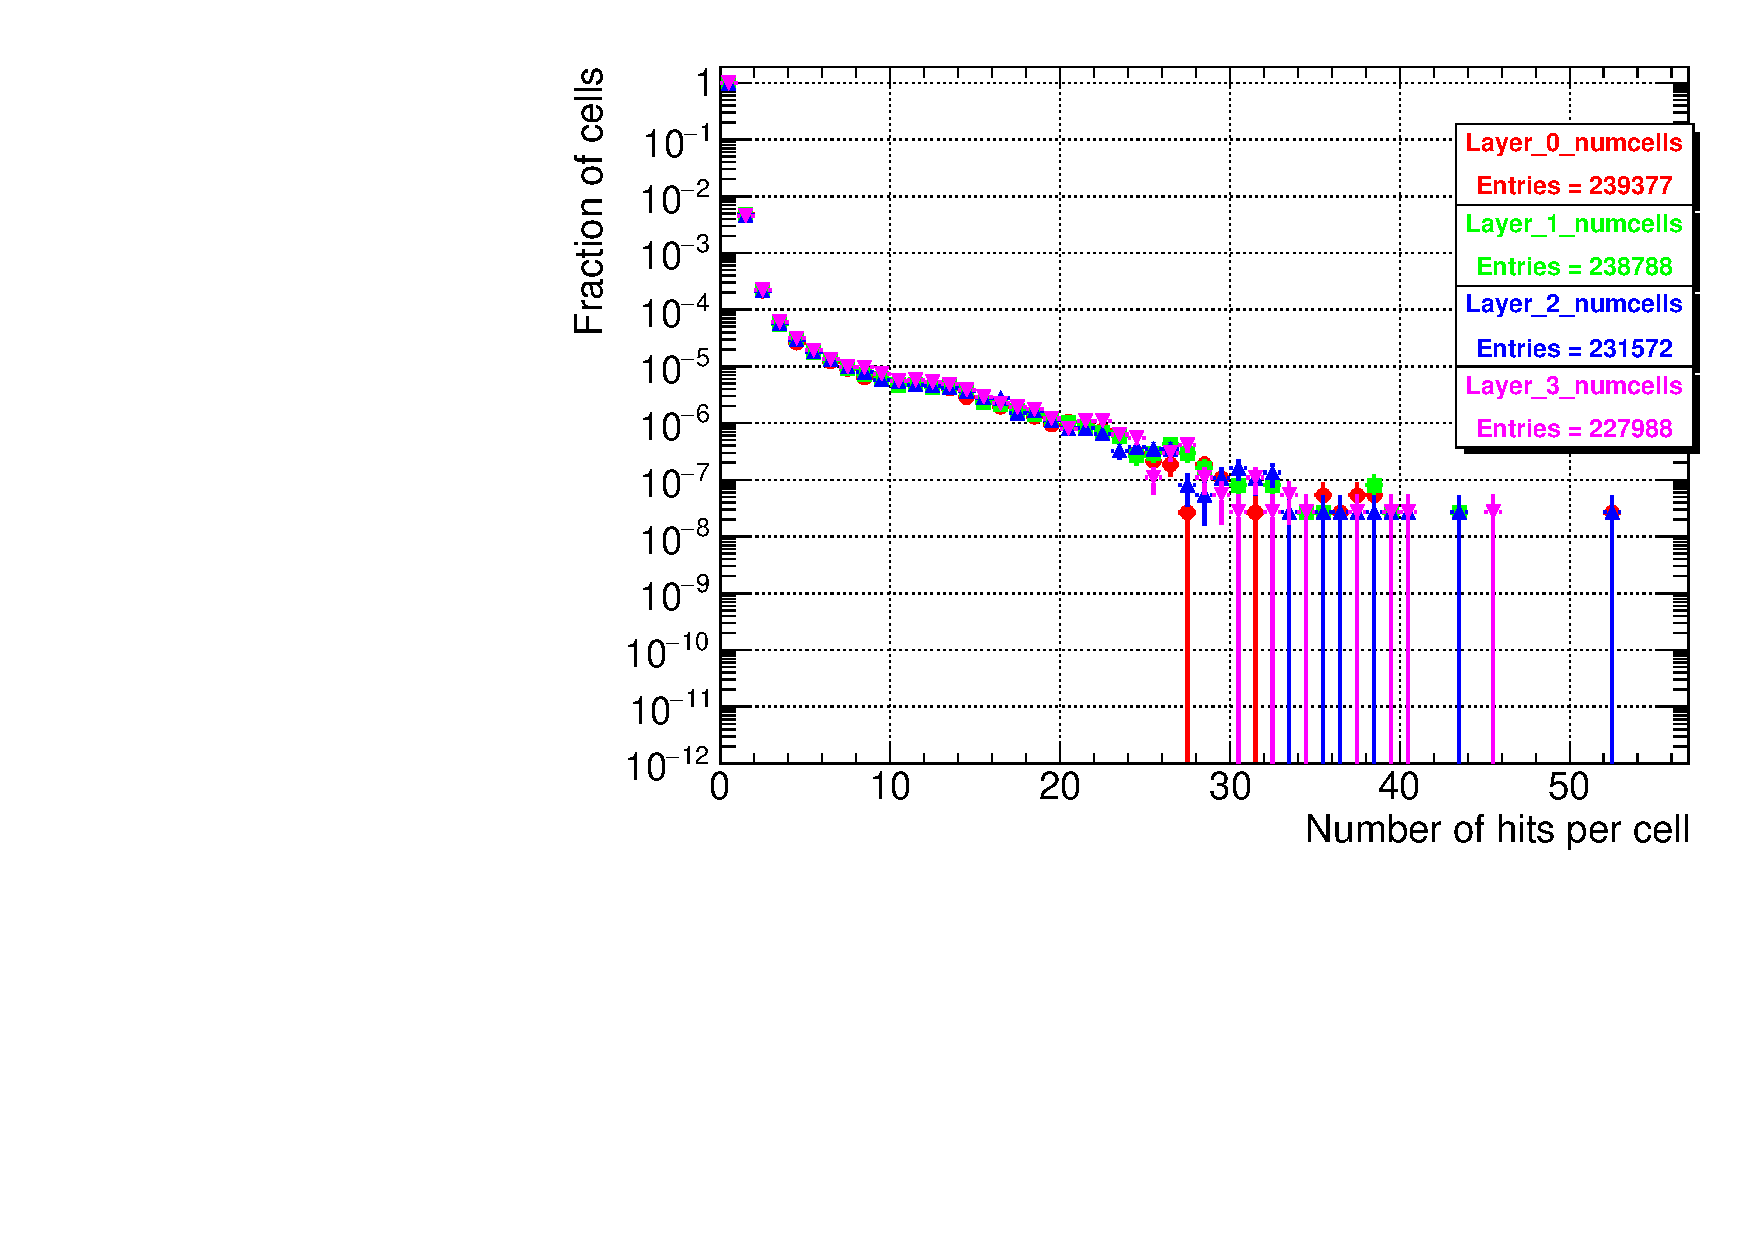
\includegraphics[width=\textwidth]{Figures/Pairs/Appendix/occupancy_numcells_SiVertexEndcap_ILC250_SetC.pdf}
   \caption{Set (C), normalized occupancy}
   \end{subfigure}
   \hfill
    \begin{subfigure}[b]{0.49\textwidth}
   \centering
    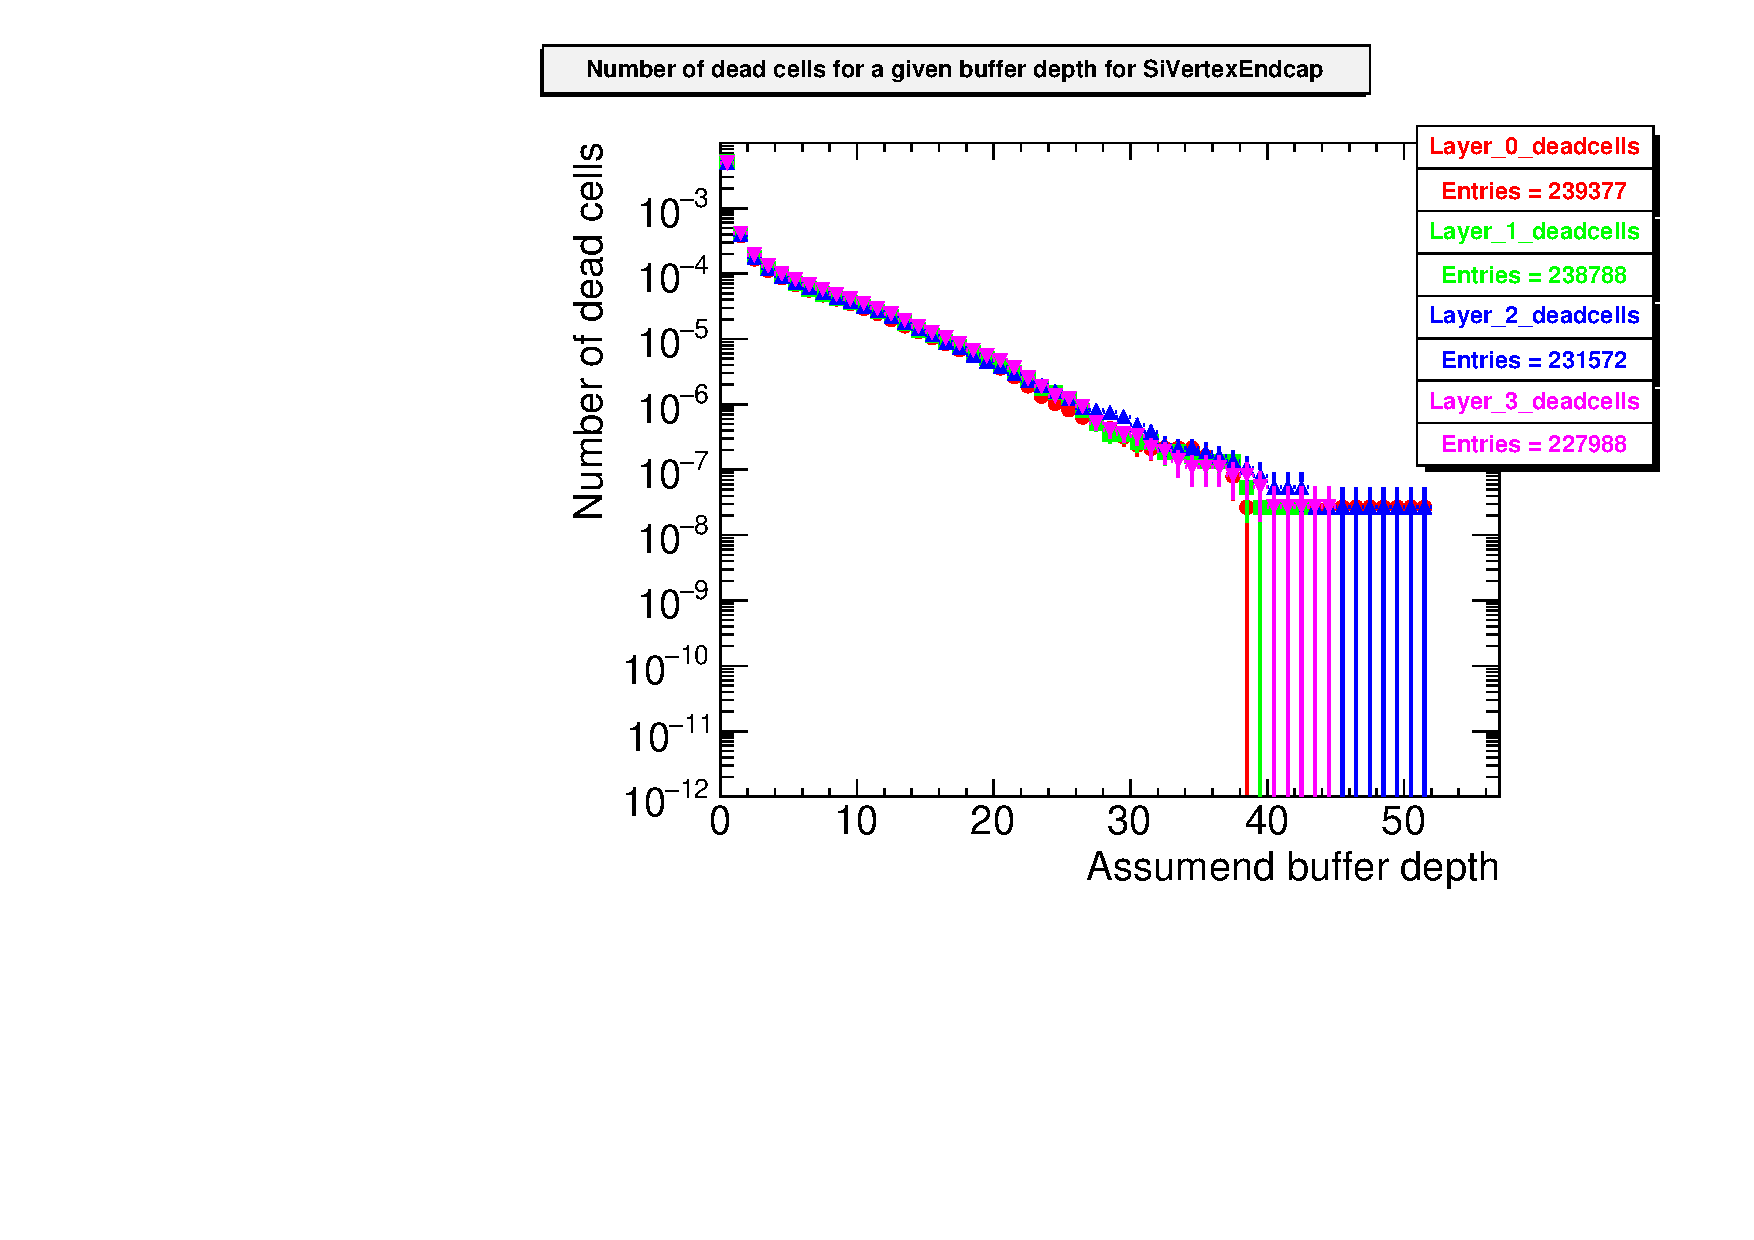
\includegraphics[width=\textwidth]{Figures/Pairs/Appendix/occupancy_deadcells_SiVertexEndcap_ILC250_SetC.pdf}
   \caption{Set (C), fraction of dead cells}
   \end{subfigure}
   \caption[Pair background occupancy in all SiD vertex detector endcap layers for the ILC250]{ILC250 pair background occupancy in all SiD vertex detector endcap layers, after a full bunch train (1312 bunch crossings).
   The left hand figures show the occupancy in the individual vertex detector layer, normalized by the total number of cells of the corresponding layer.
   The right hand figures show the fraction of the dead cells in the individual vertex detector layer, with respect to the total number of cells.
   \\The dashed lines indicate the the buffer depth of four for the current sensor design, and the guideline of \num{e-4} for a critical acceptance limit.
   }
   %\label{fig:PairBkg:ILC250_Occupancy_Layers_VXDEndcap}
 \end{figure}
 
 \clearpage
 \subsection{Pair background occupancy in further \sid subdetectors}

\begin{figure}[!htbp]
 \centering
  \begin{subfigure}[b]{0.49\textwidth}
   \centering
    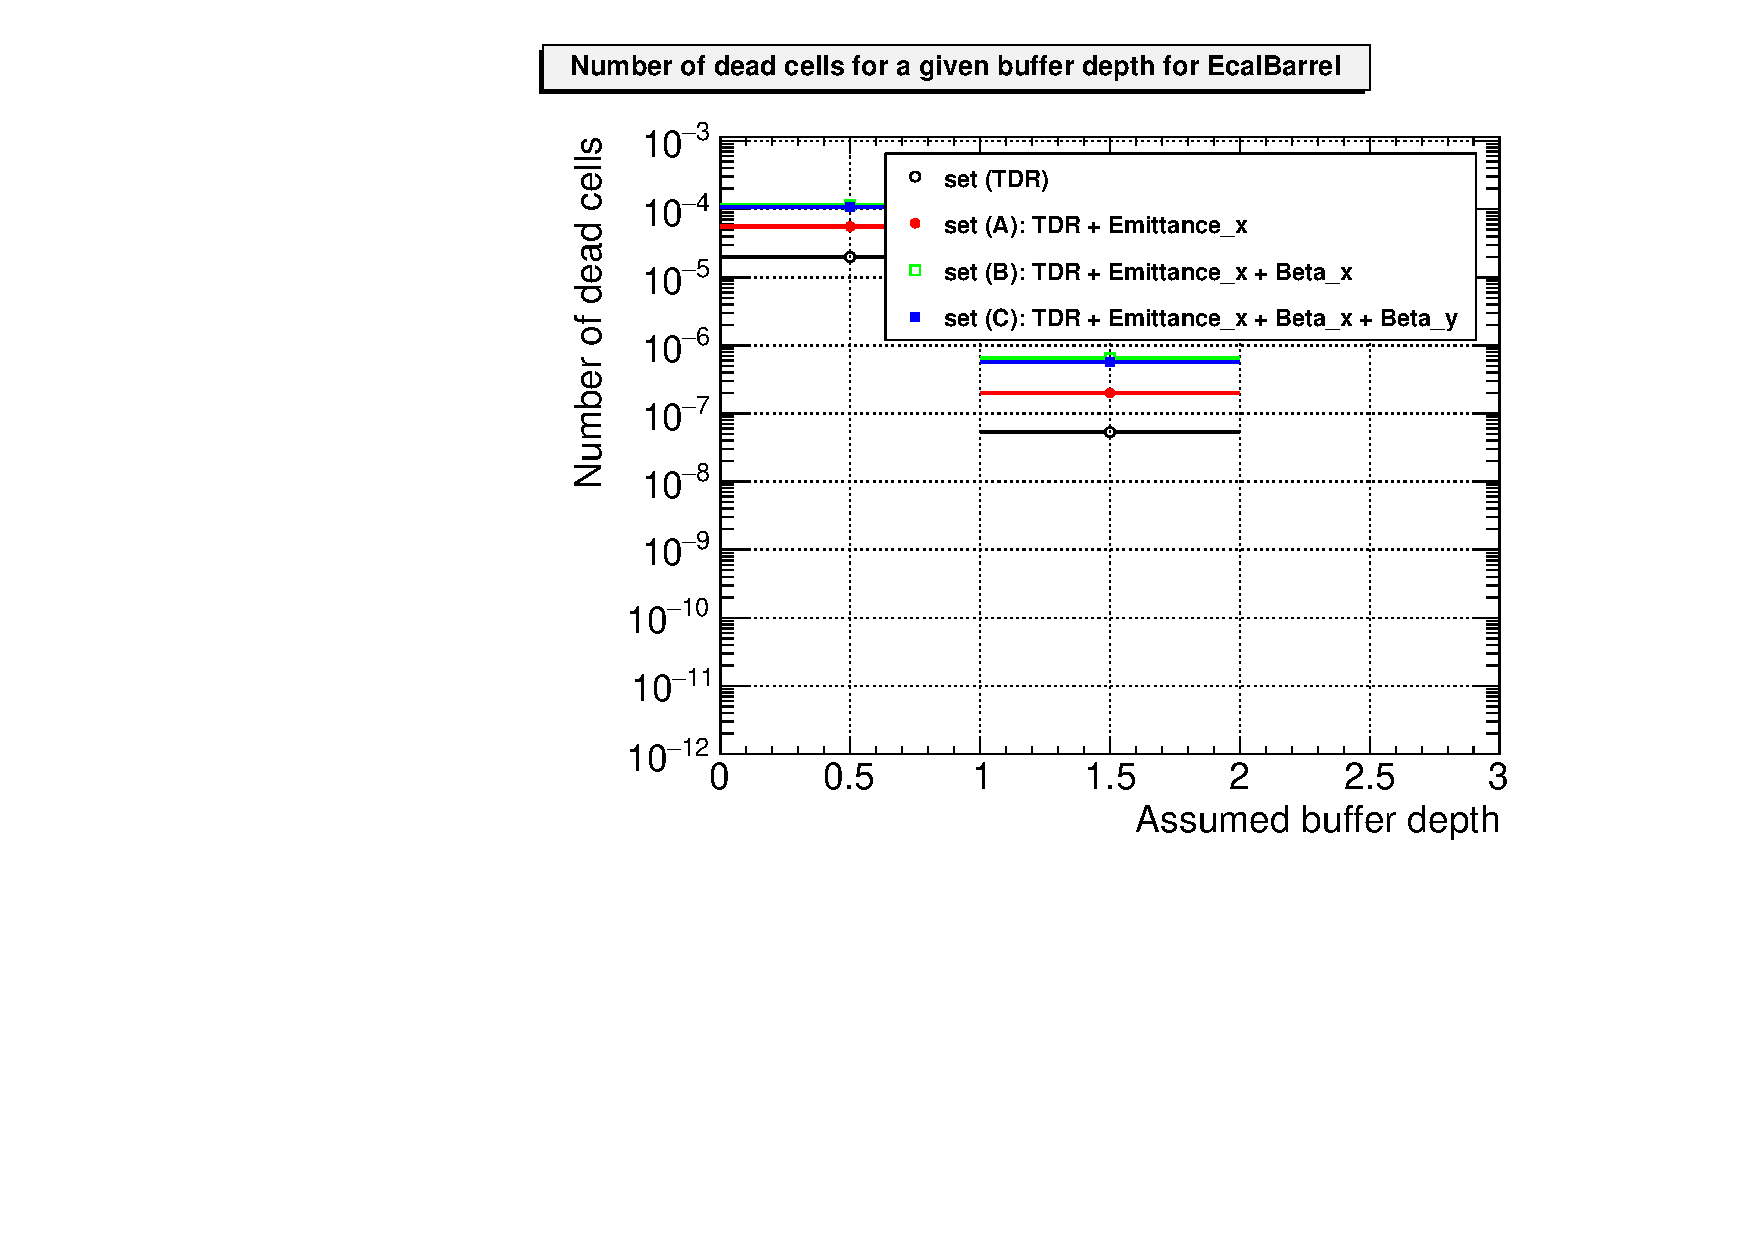
\includegraphics[width=\textwidth]{Figures/Pairs/Appendix/Occupancy_Comparison_All_layers_deadcells_ILC250_ALL_SETS_ECALBarrel.pdf}
   \caption{\sid ECAL barrel}
   \end{subfigure}
   \hfill
     \begin{subfigure}[b]{0.49\textwidth}
   \centering
    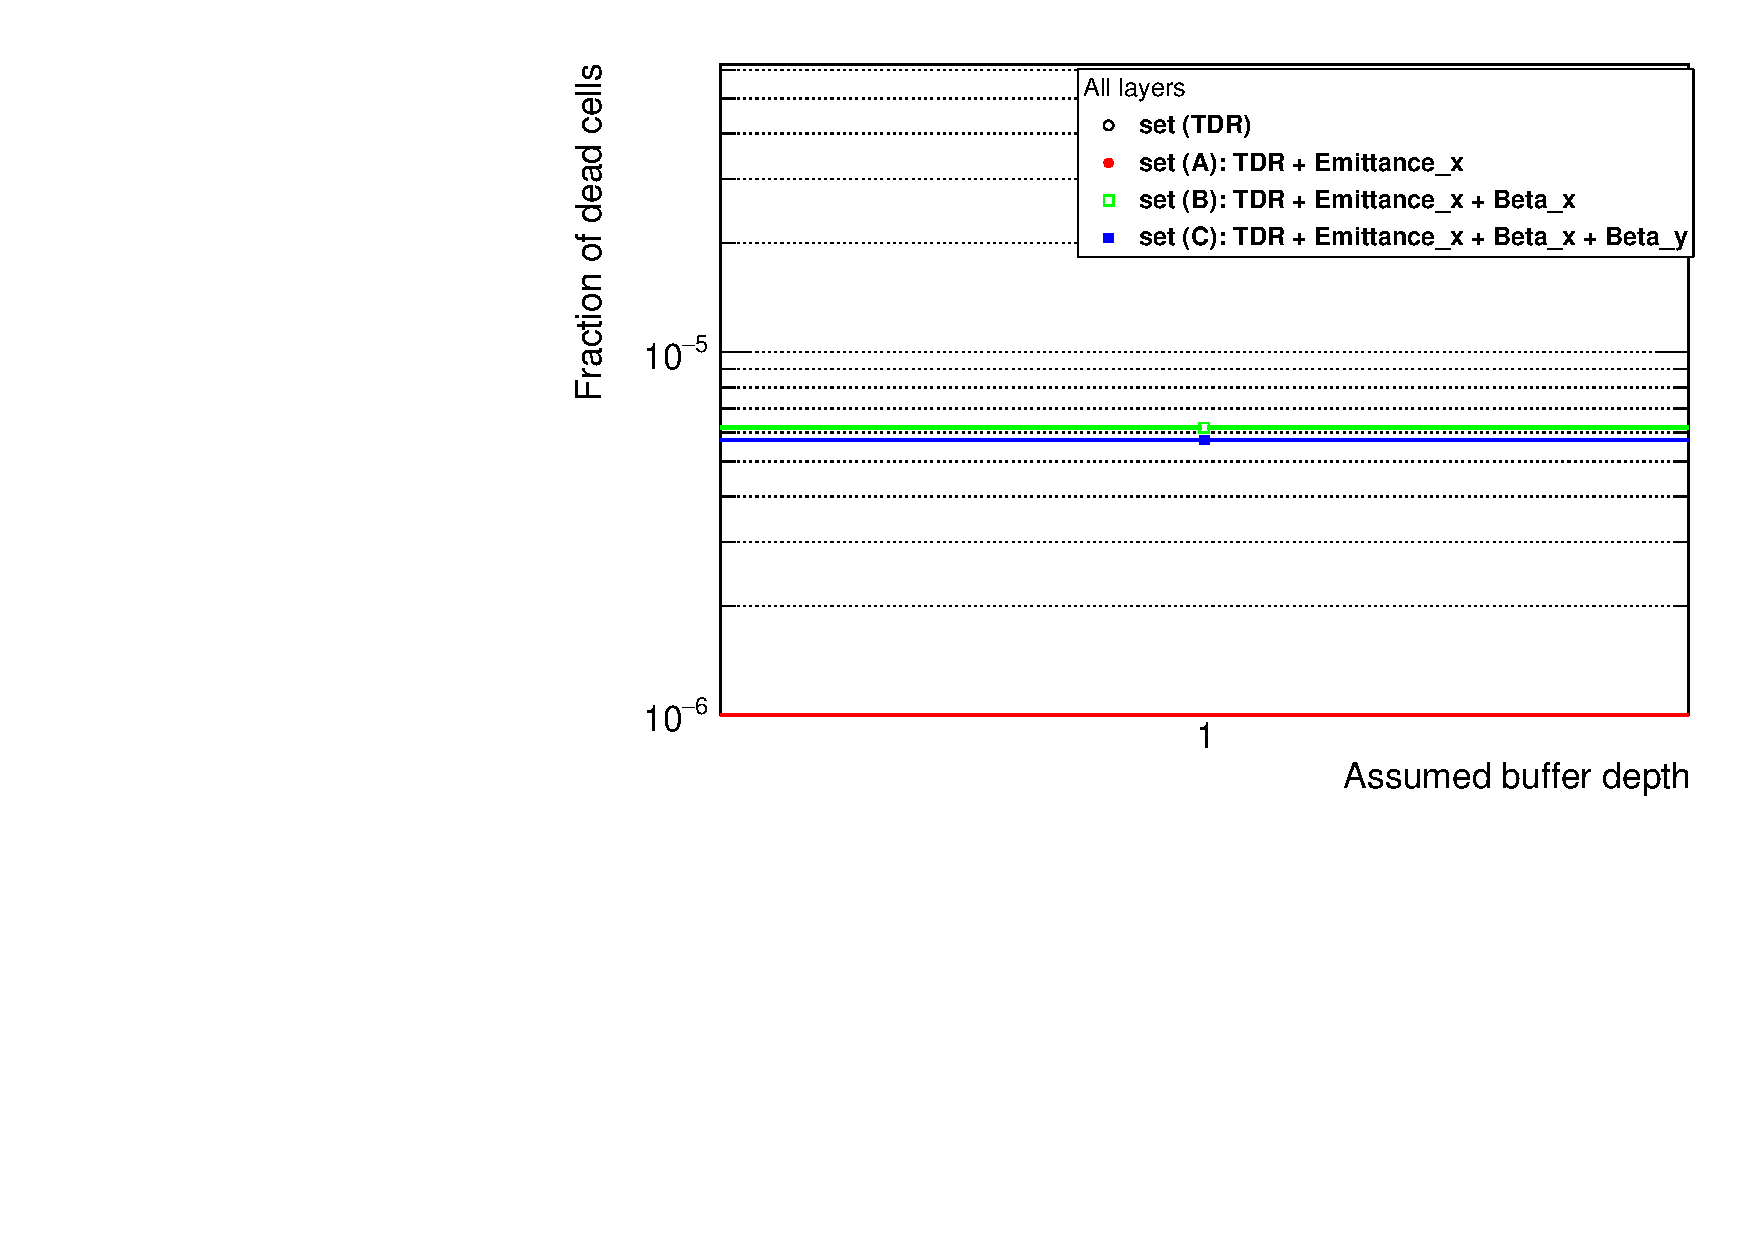
\includegraphics[width=\textwidth]
    {Figures/Pairs/Appendix/Occupancy_Comparison_All_layers_deadcells_ILC250_ALL_SETS_HcalBarrel.pdf}
   \caption{\sid HCAL barrel}
   \end{subfigure}
   \caption[Pair background occupancy in the \sid calorimater barrels for the ILC250]{ILC250 pair background occupancy in the \sid calorimeter barrels after a full bunch train (1312 bunch crossings).
   The figures show the fraction of the dead cells in the individual subdetectors for all layers combined, with respect to the total number of cells in this subdetector.
   \\The dashed lines indicate the the buffer depth of four for the current sensor design, and the guideline of \num{e-4} for a critical acceptance limit.
   }
   \label{fig:PairBkg:ILC250_Occupancy_Further_detectors}
\end{figure}

\chapter{Muon background from the Beam Delivery System}
\label{Appendix:BDS_Muons}
Figure~\ref{fig:BDS_Muons:occupancies} shows occupancy plots belonging to the study of the muons from the Beam Delivery System (BDS) presented in Chapter~\ref{BDS_Muons}.
  \begin{figure}[htbp]
 \centering
  \begin{subfigure}[b]{0.49\textwidth}
   \centering
    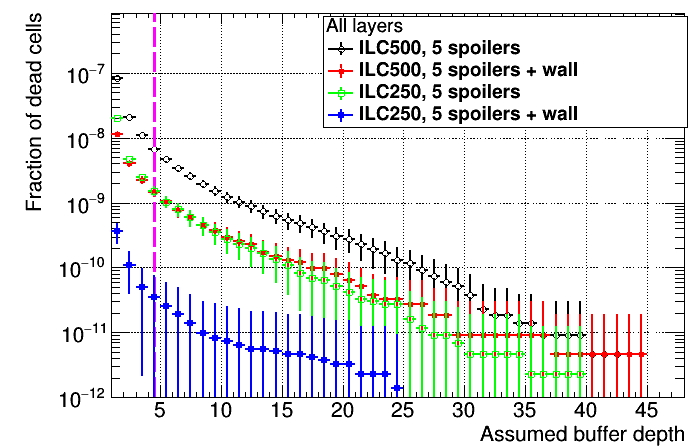
\includegraphics[width=\textwidth]{Figures/BDS_muons/Occupancy_Comparison_All_layers_deadcells_SiTrackerBarrel.png}
   \caption{\sid Tracker barrel}
   \end{subfigure}
   \hfill
    \begin{subfigure}[b]{0.49\textwidth}
   \centering
    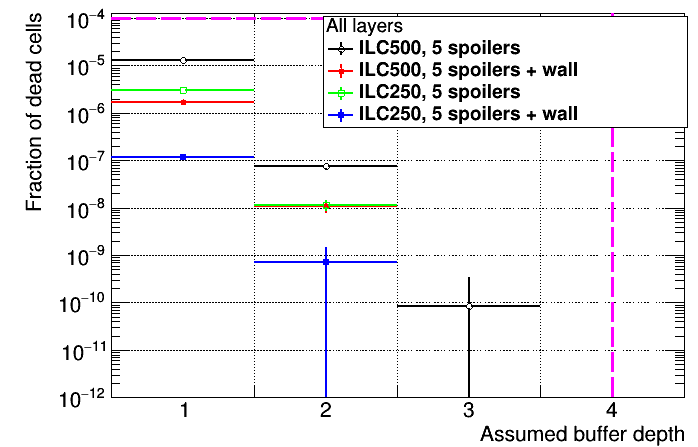
\includegraphics[width=\textwidth]{Figures/BDS_muons/Occupancy_Comparison_All_layers_deadcells_EcalBarrel.png}
   \caption{\sid ECAL barrel}
   \end{subfigure}
         \caption[Occupancy from BDS muons of various SiD subdetectors]{
   BDS muon background occupancy in the \sid subdetectors after a full bunch train (1312 bunch crossings).   
   The plots show the fraction of dead cells with respect to the total number of cells in the respective SiD subdetector.
   \\The dashed lines indicate the the buffer depth of four for the current sensor design, and the guideline of \num{e-4} for a critical acceptance limit.}
   \label{fig:BDS_Muons:occupancies}
     \end{figure}
  \begin{figure}[htb]\ContinuedFloat
   \begin{subfigure}[b]{0.49\textwidth}
   \centering
    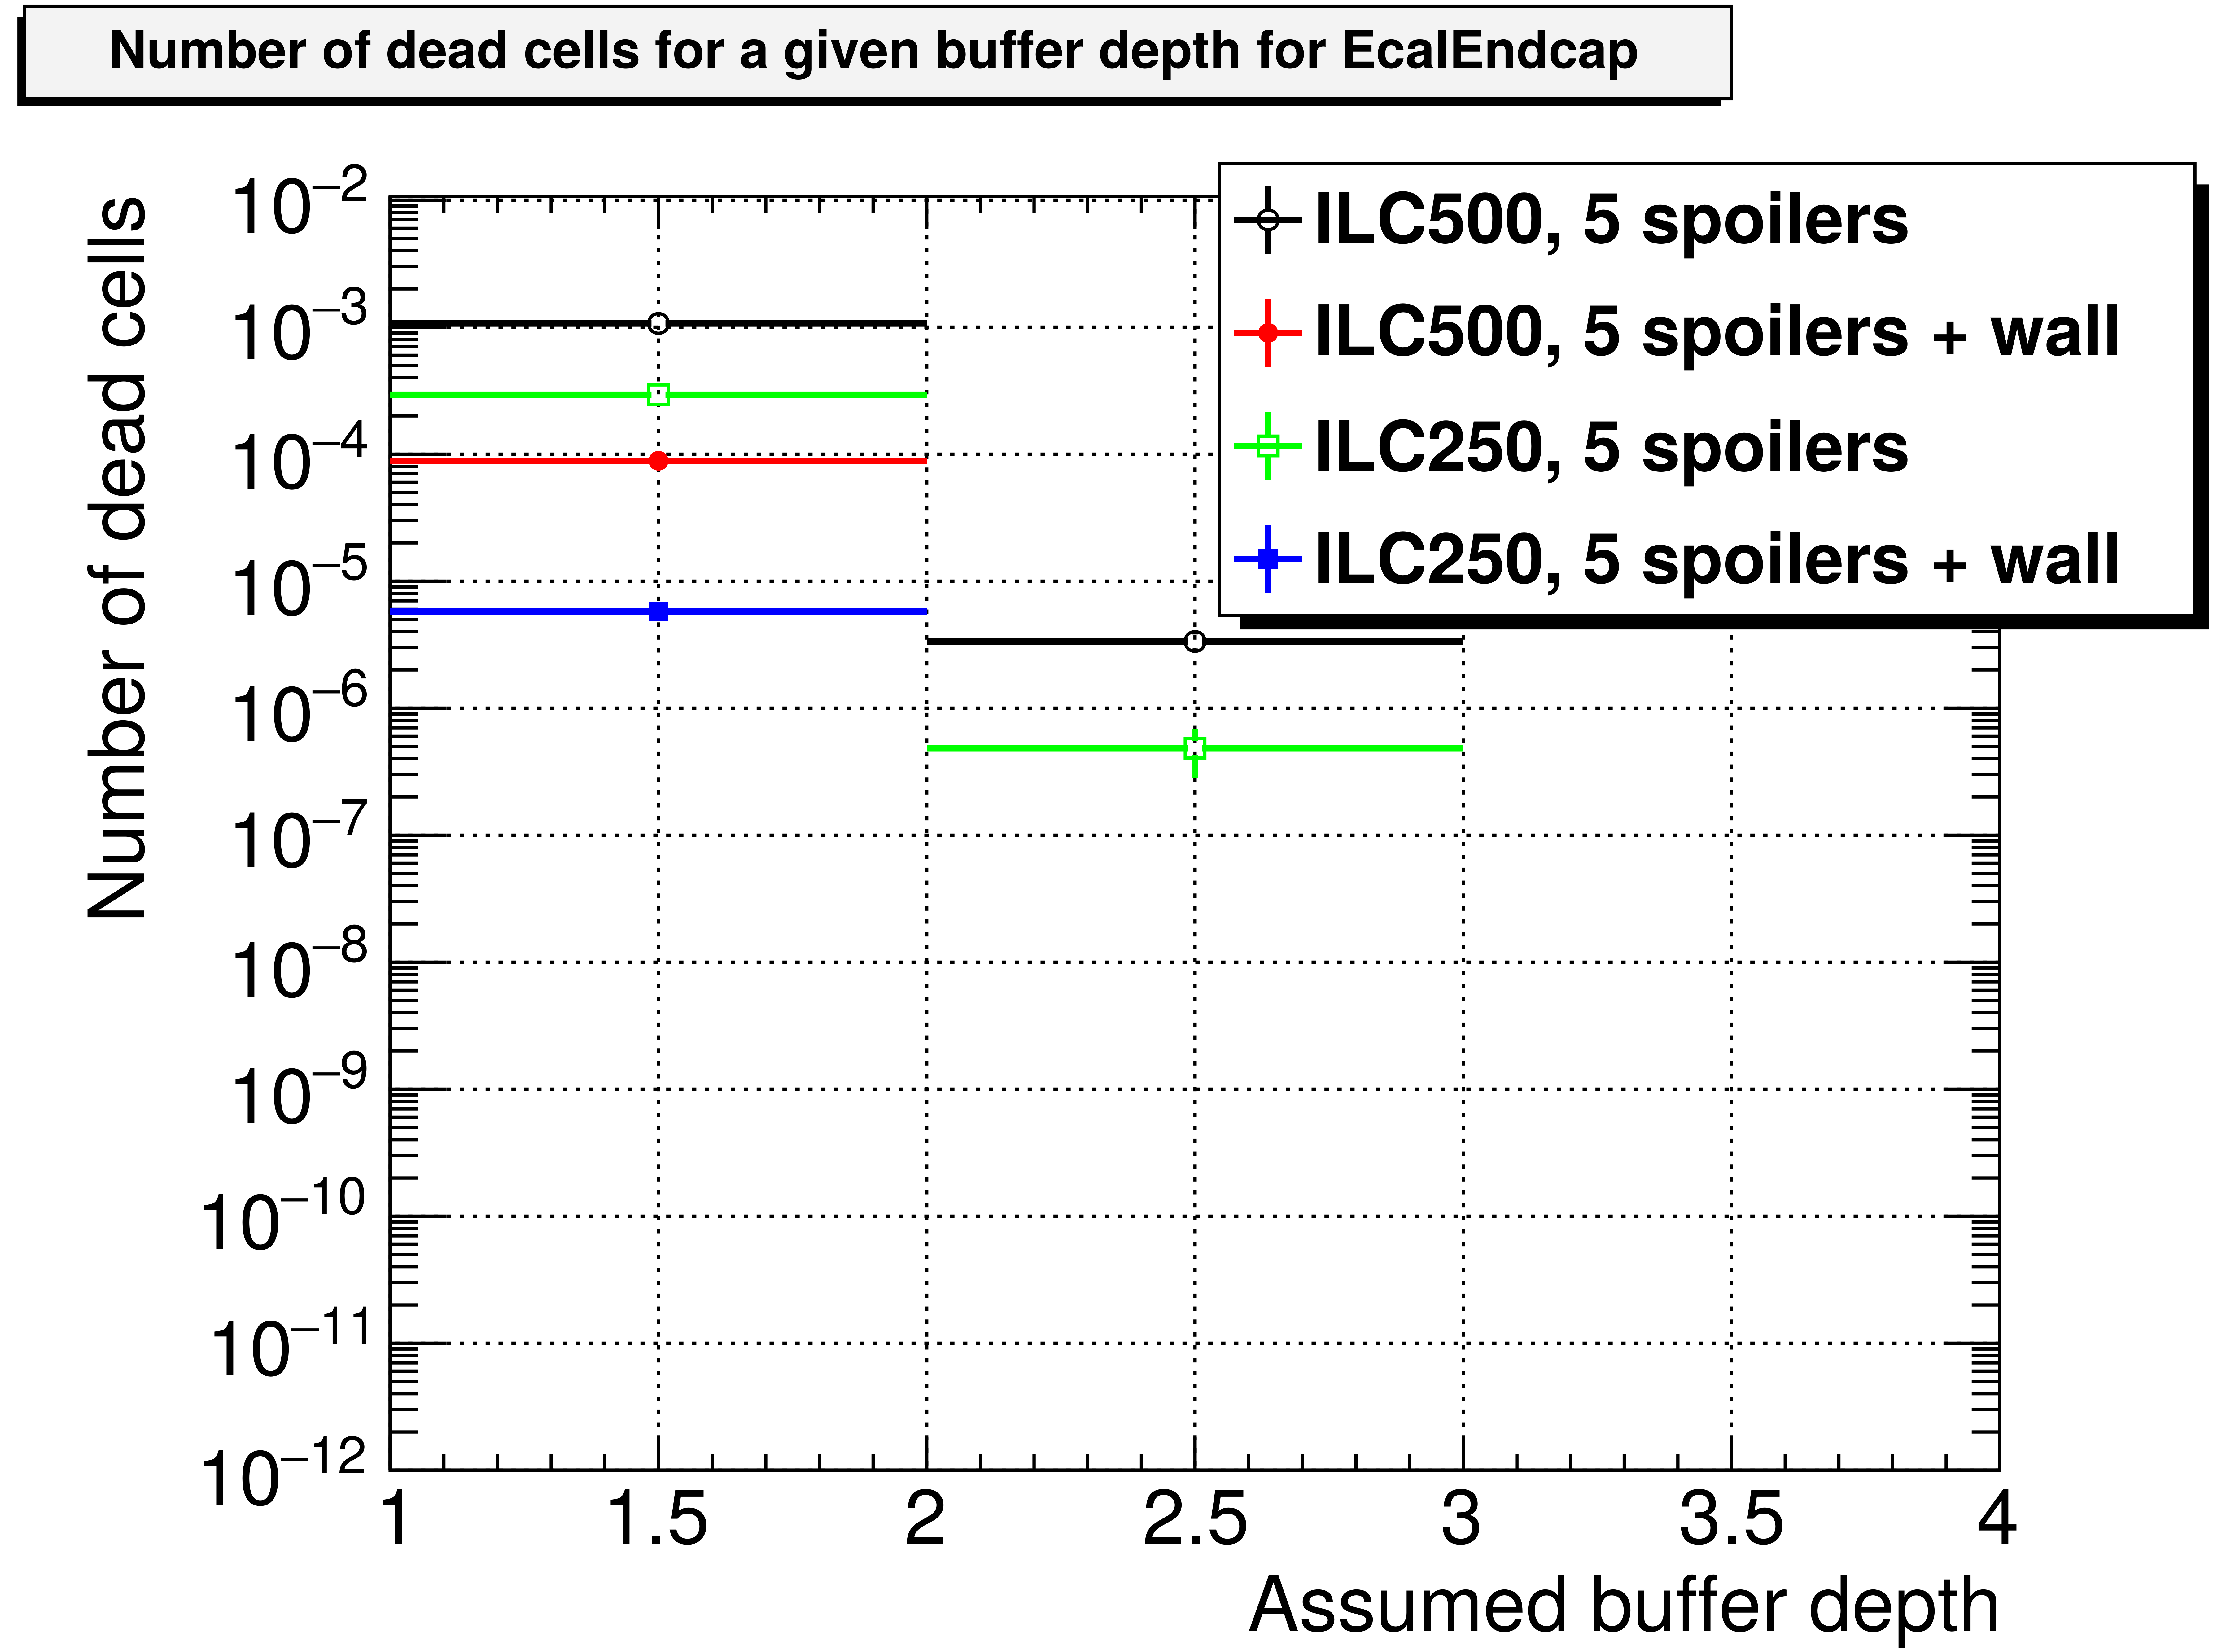
\includegraphics[width=\textwidth]{Figures/BDS_muons/Occupancy_Comparison_All_layers_deadcells_EcalEndcap.png}
   \caption{\sid ECAL endcap}
   \end{subfigure}
   \hfill
    \begin{subfigure}[b]{0.49\textwidth}
   \centering
    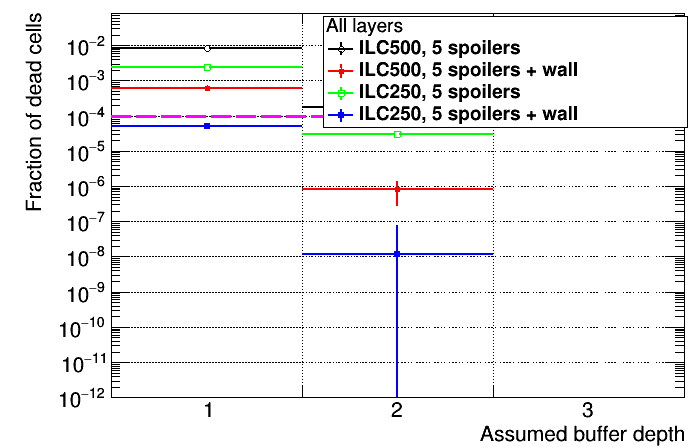
\includegraphics[width=\textwidth]{Figures/BDS_muons/Occupancy_Comparison_All_layers_deadcells_HcalEndcap.png}
   \caption{\sid HCAL endcap}
   \end{subfigure}\\
   \begin{subfigure}[b]{0.49\textwidth}
   \centering
    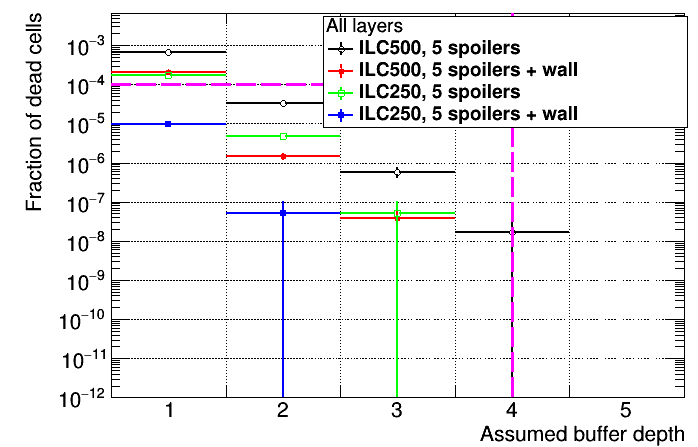
\includegraphics[width=\textwidth]{Figures/BDS_muons/Occupancy_Comparison_All_layers_deadcells_MuonBarrel.png}
   \caption{\sid Muon system barrel}
   \end{subfigure}
   \hfill
    \begin{subfigure}[b]{0.49\textwidth}
   \centering
    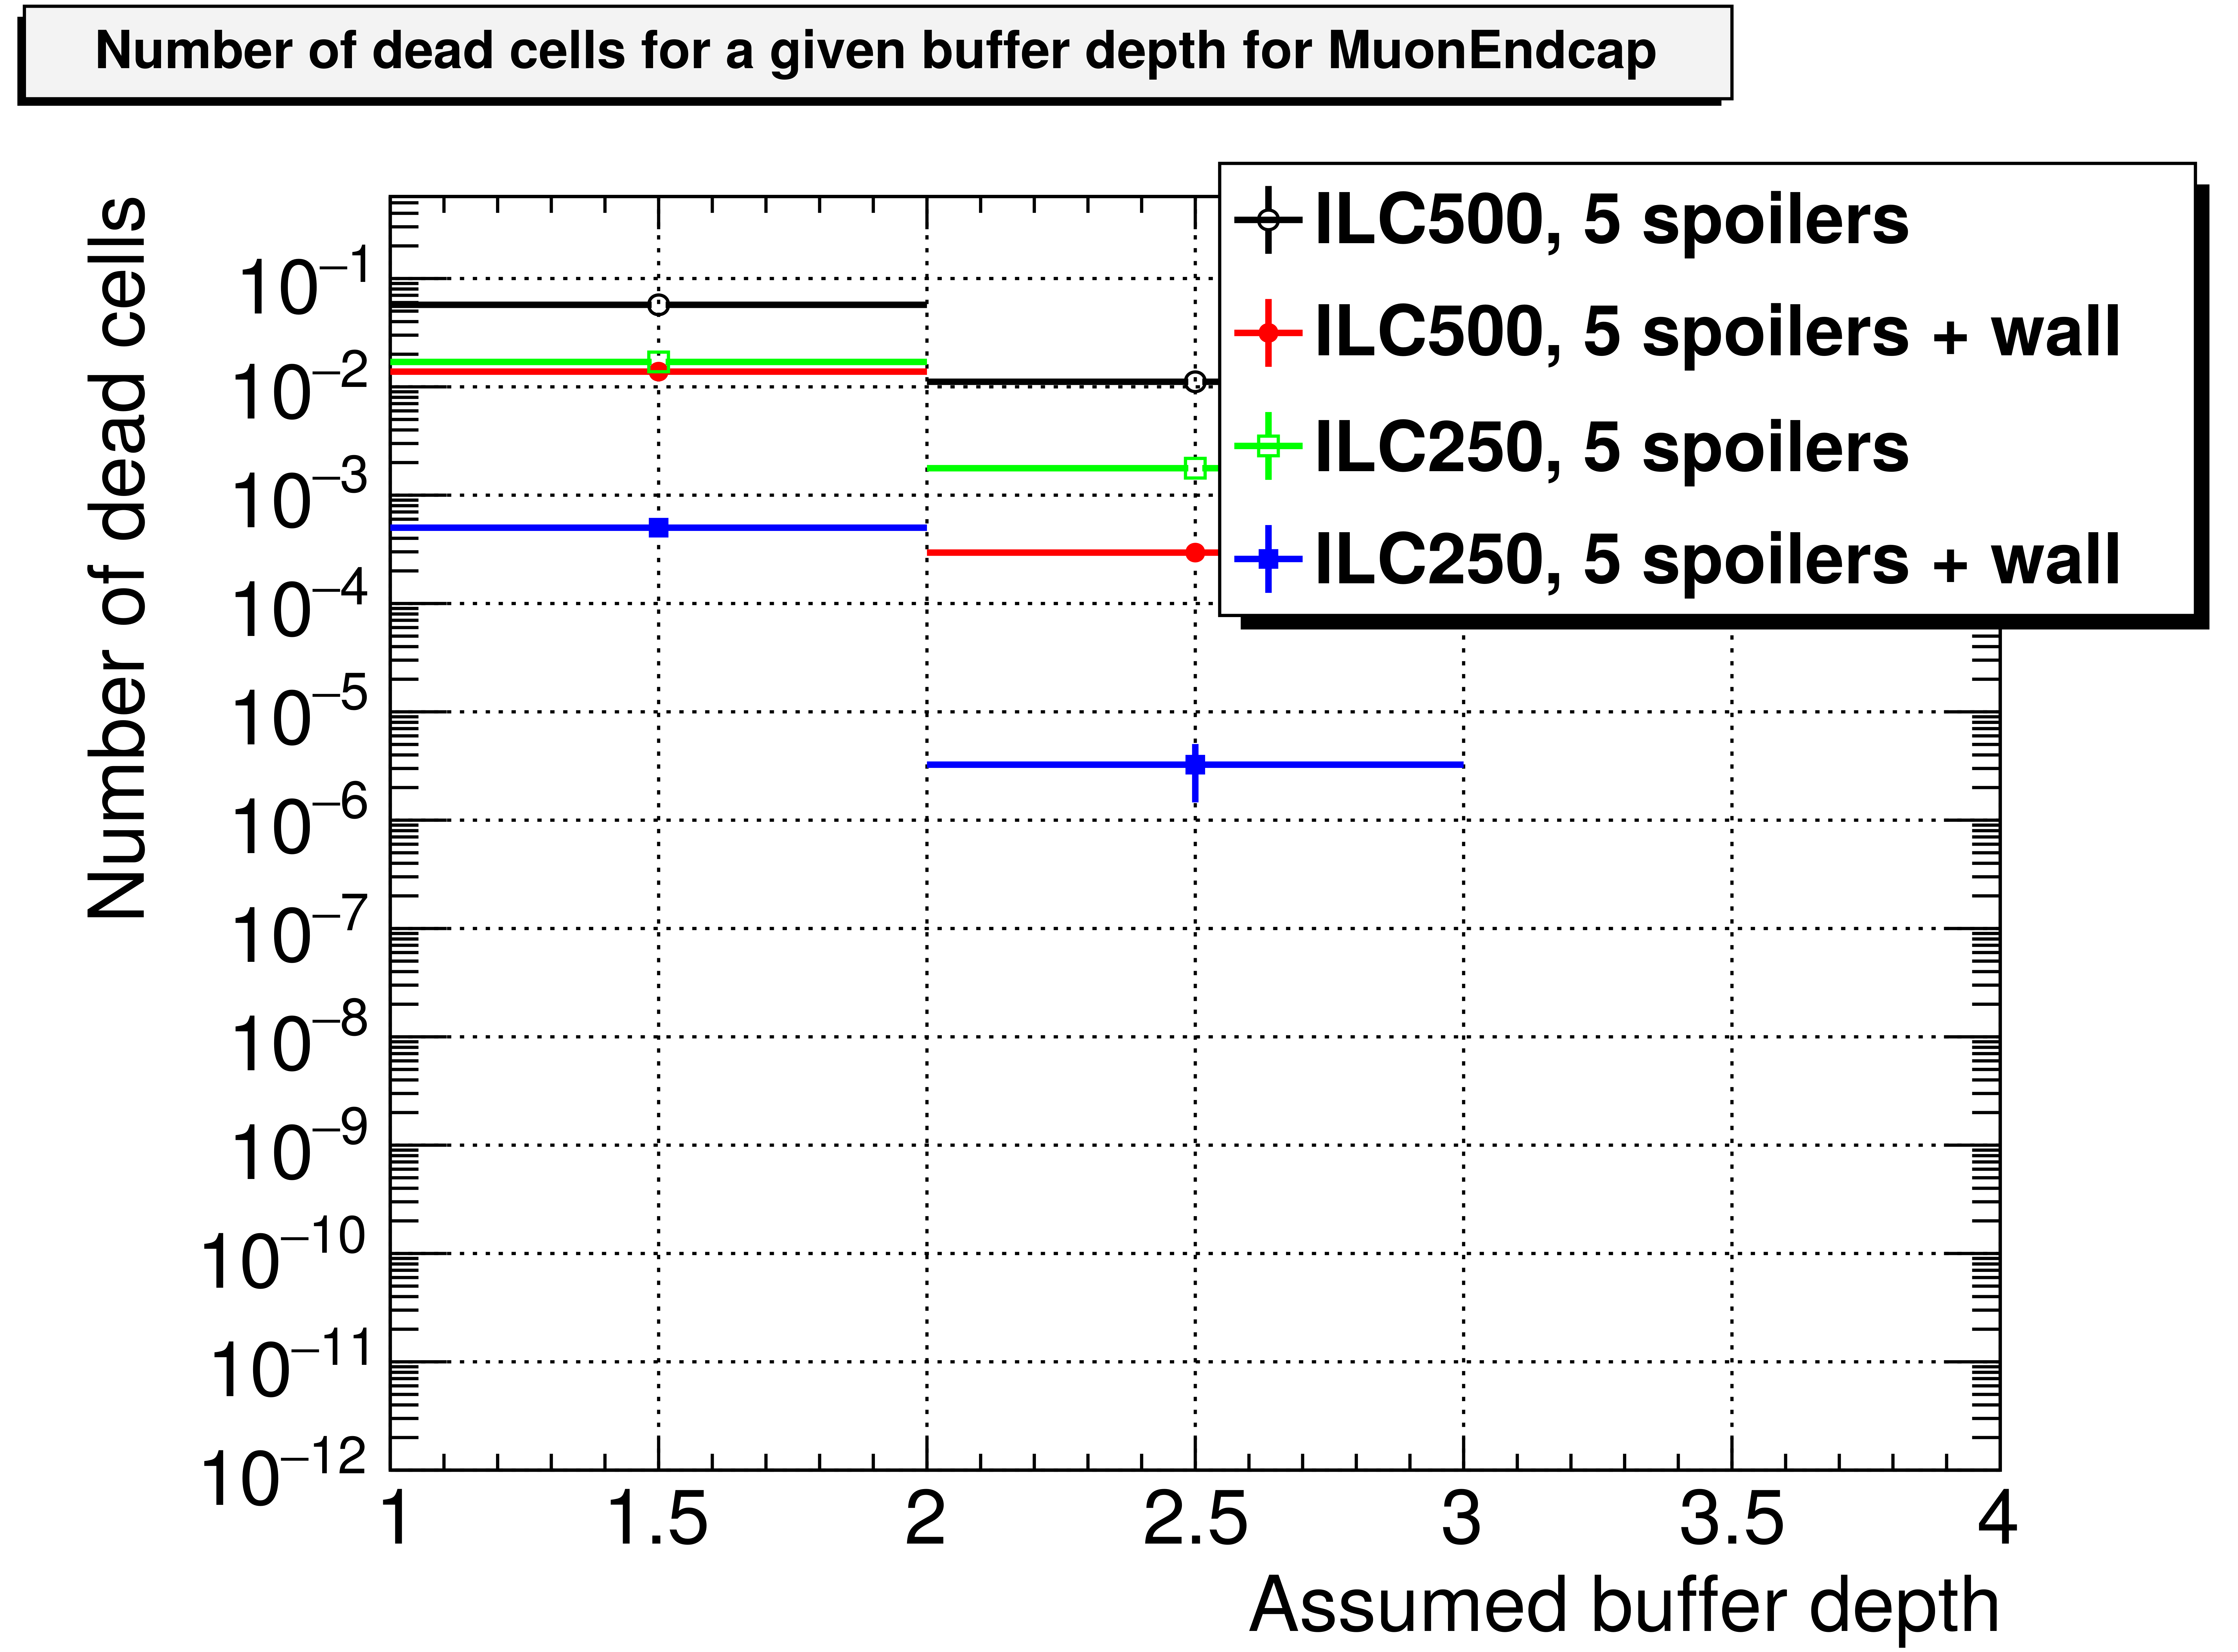
\includegraphics[width=\textwidth]{Figures/BDS_muons/Occupancy_Comparison_All_layers_deadcells_MuonEndcap.png}
   \caption{\sid Muon system endcap}
   \end{subfigure}\\
     \begin{subfigure}[b]{0.49\textwidth}
   \centering
    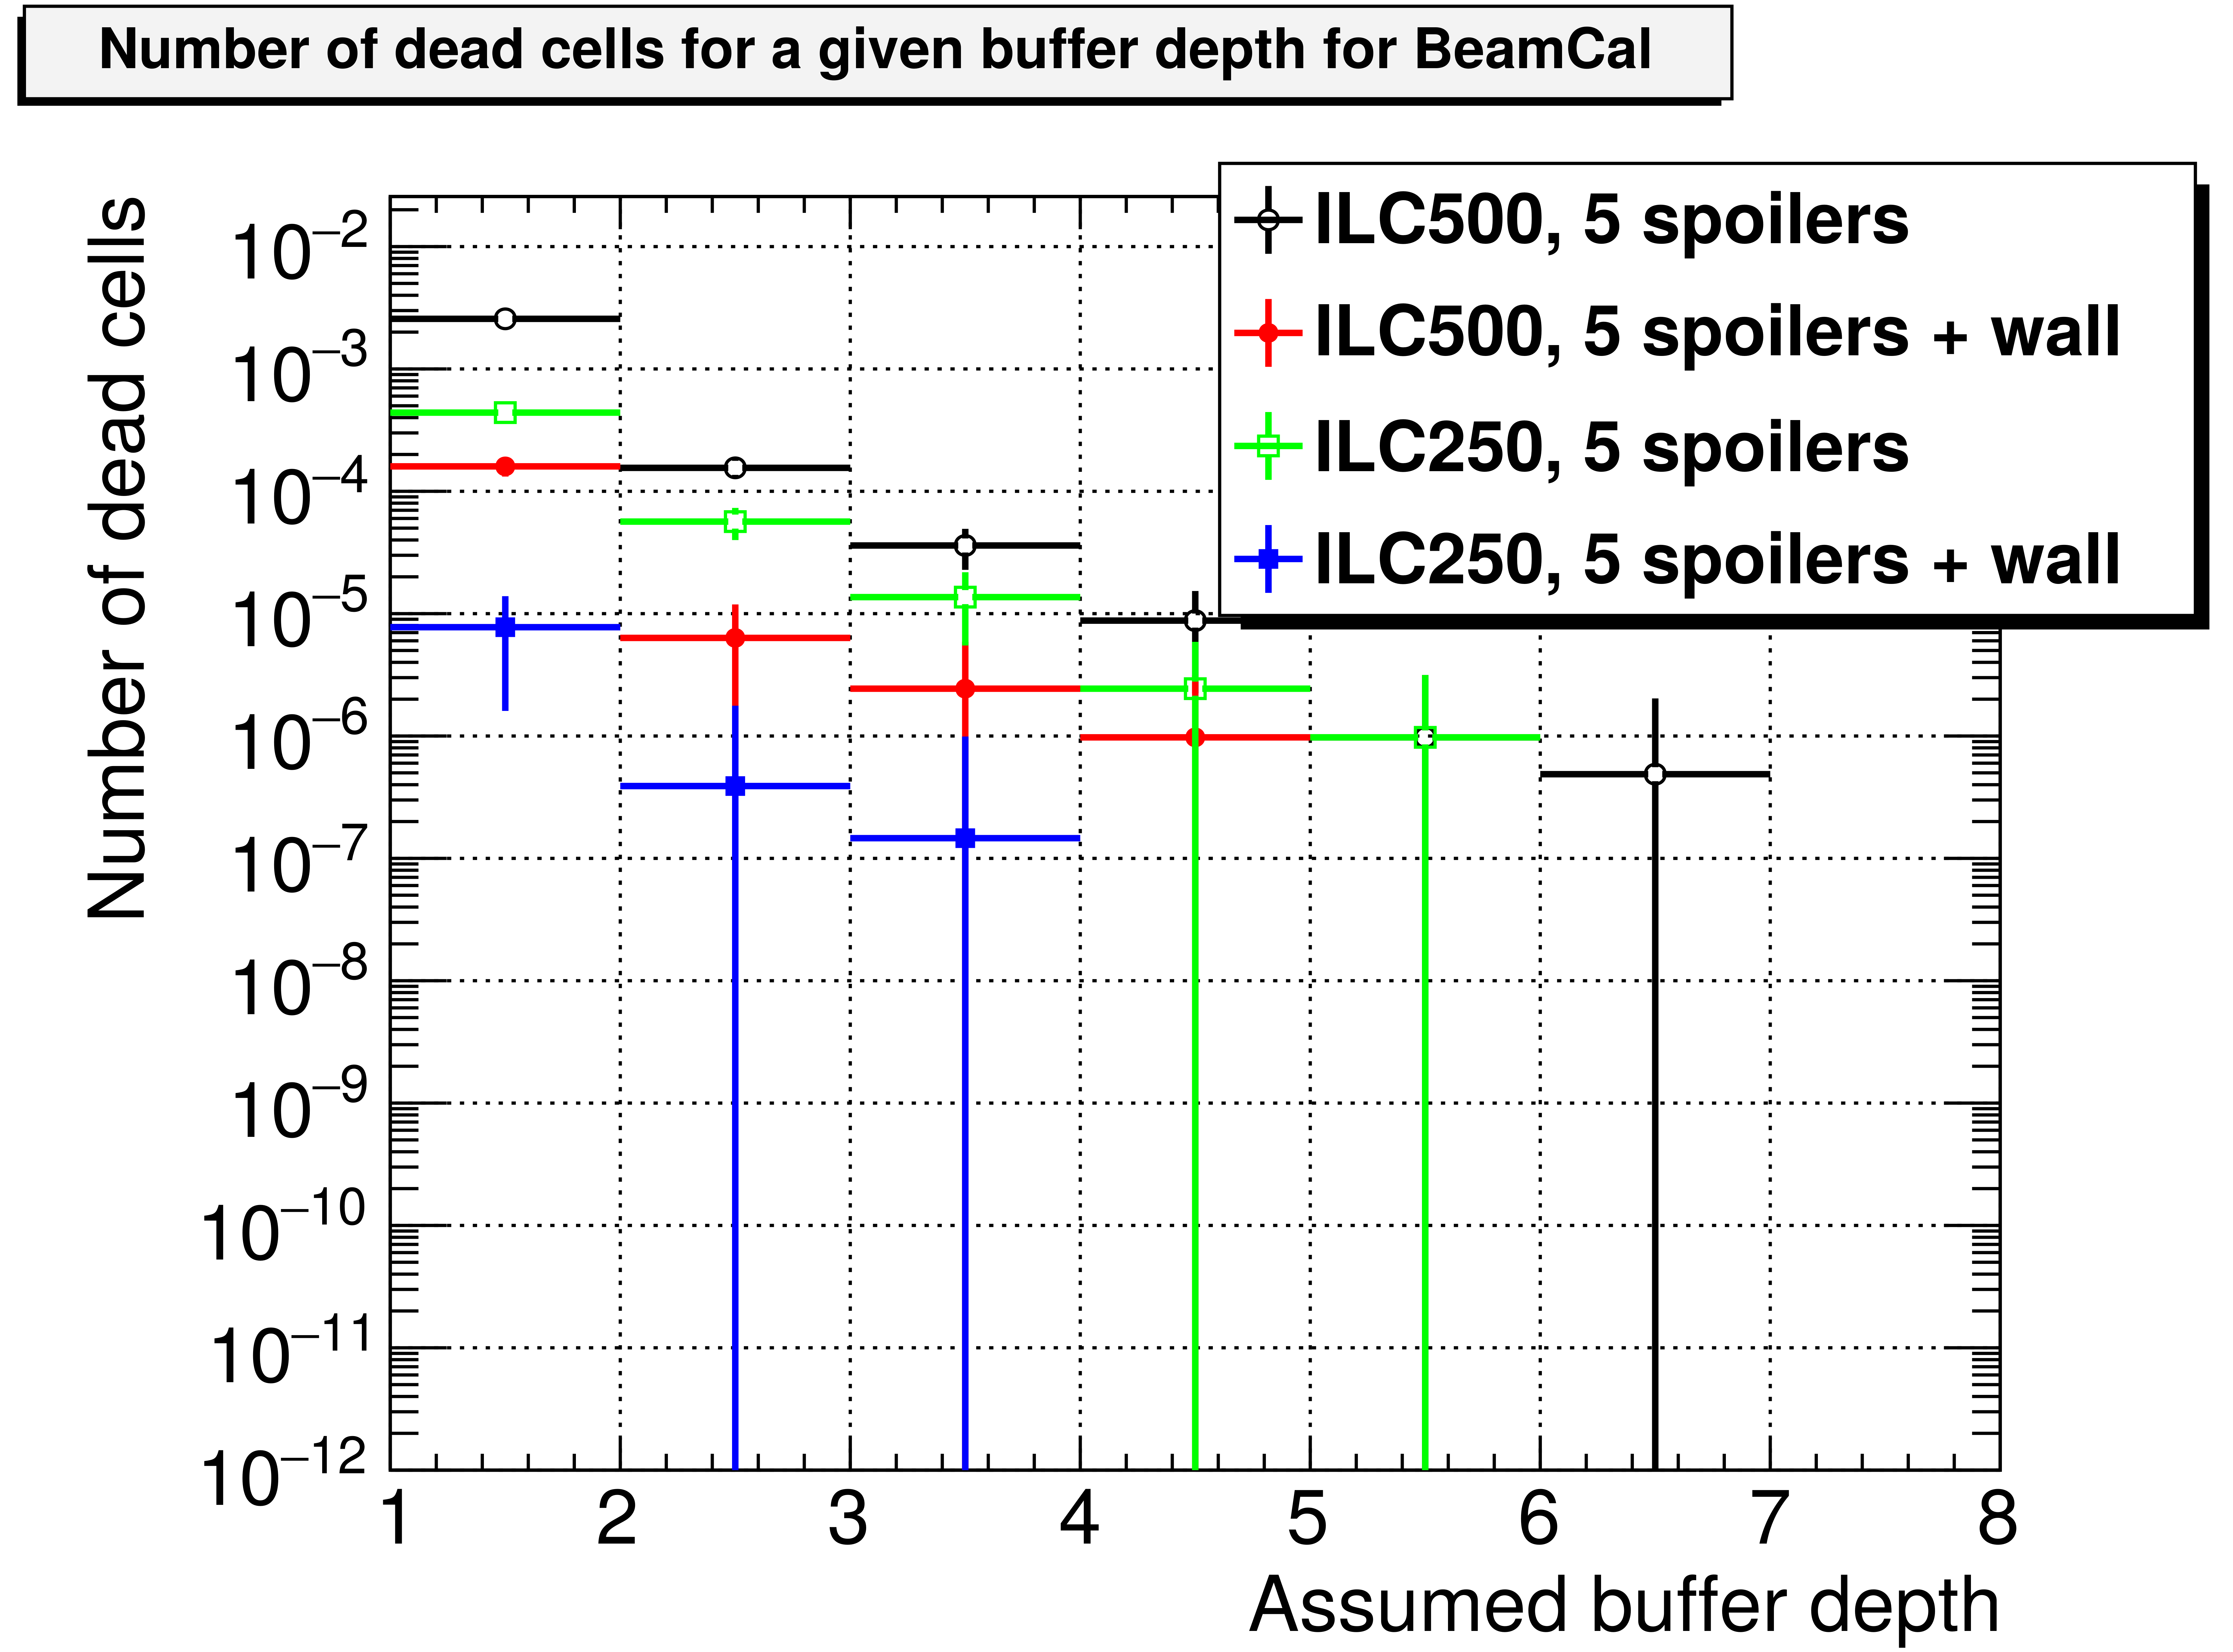
\includegraphics[width=\textwidth]{Figures/BDS_muons/Occupancy_Comparison_All_layers_deadcells_BeamCal.png}
   \caption{\sid BeamCal}
   \end{subfigure}
   \hfill
    \begin{subfigure}[b]{0.49\textwidth}
   \centering
    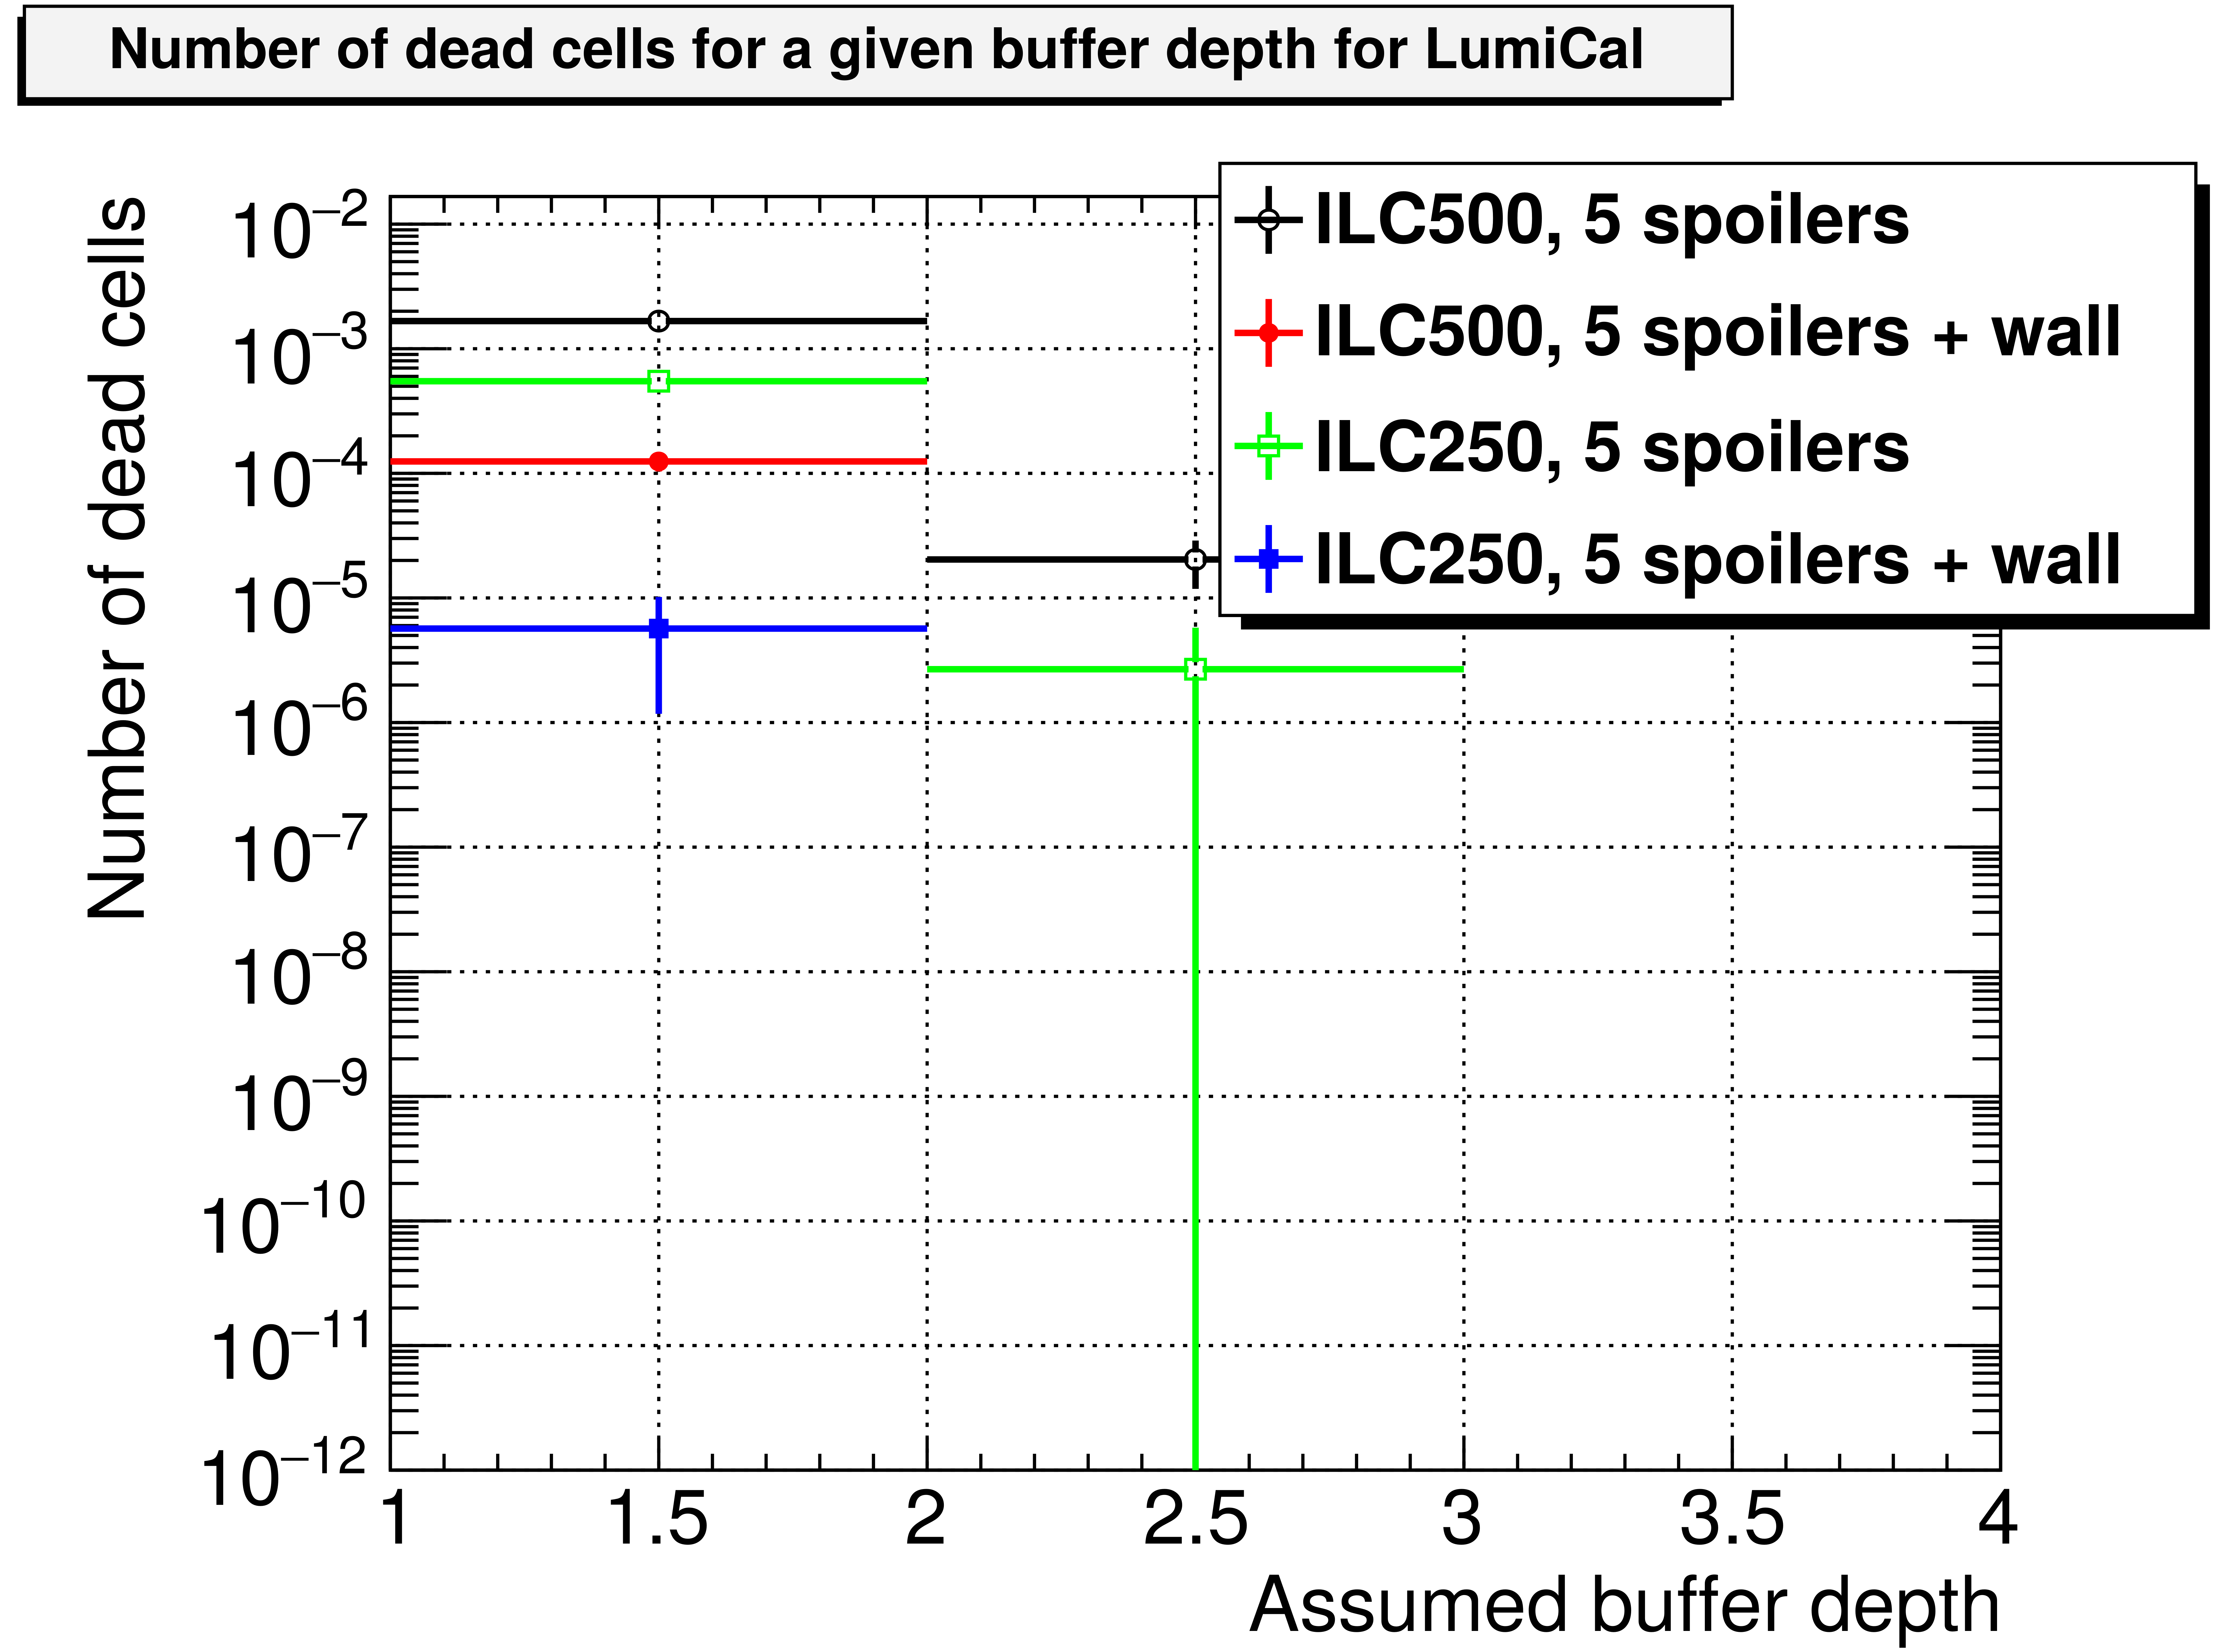
\includegraphics[width=\textwidth]{Figures/BDS_muons/Occupancy_Comparison_All_layers_deadcells_LumiCal.png}
   \caption{\sid LumiCal}
   \end{subfigure}
   \caption[Occupancy from BDS muons of various SiD subdetectors]{
   BDS muon background occupancy in the \sid subdetectors after a full bunch train (1312 bunch crossings).   
   The plots show the fraction of dead cells with respect to the total number of cells in the respective SiD subdetector.
   \\The dashed lines indicate the the buffer depth of four for the current sensor design, and the guideline of \num{e-4} for a critical acceptance limit.}
  % \label{fig:BDS_Muons:occupancies}
 \end{figure}
 
\chapter{Background from the main beam dumps}
\label{Appendix:BeamDump}
\begin{figure}[!h]
 \centering
  \begin{subfigure}[b]{0.49\textwidth}
   \centering
    \includegraphics[width=\textwidth]{Figures/BeamDump/Design1_1.png}
   \caption{\designone, 1 minute}
   \end{subfigure}
   \hfill
    \begin{subfigure}[b]{0.49\textwidth}
   \centering
    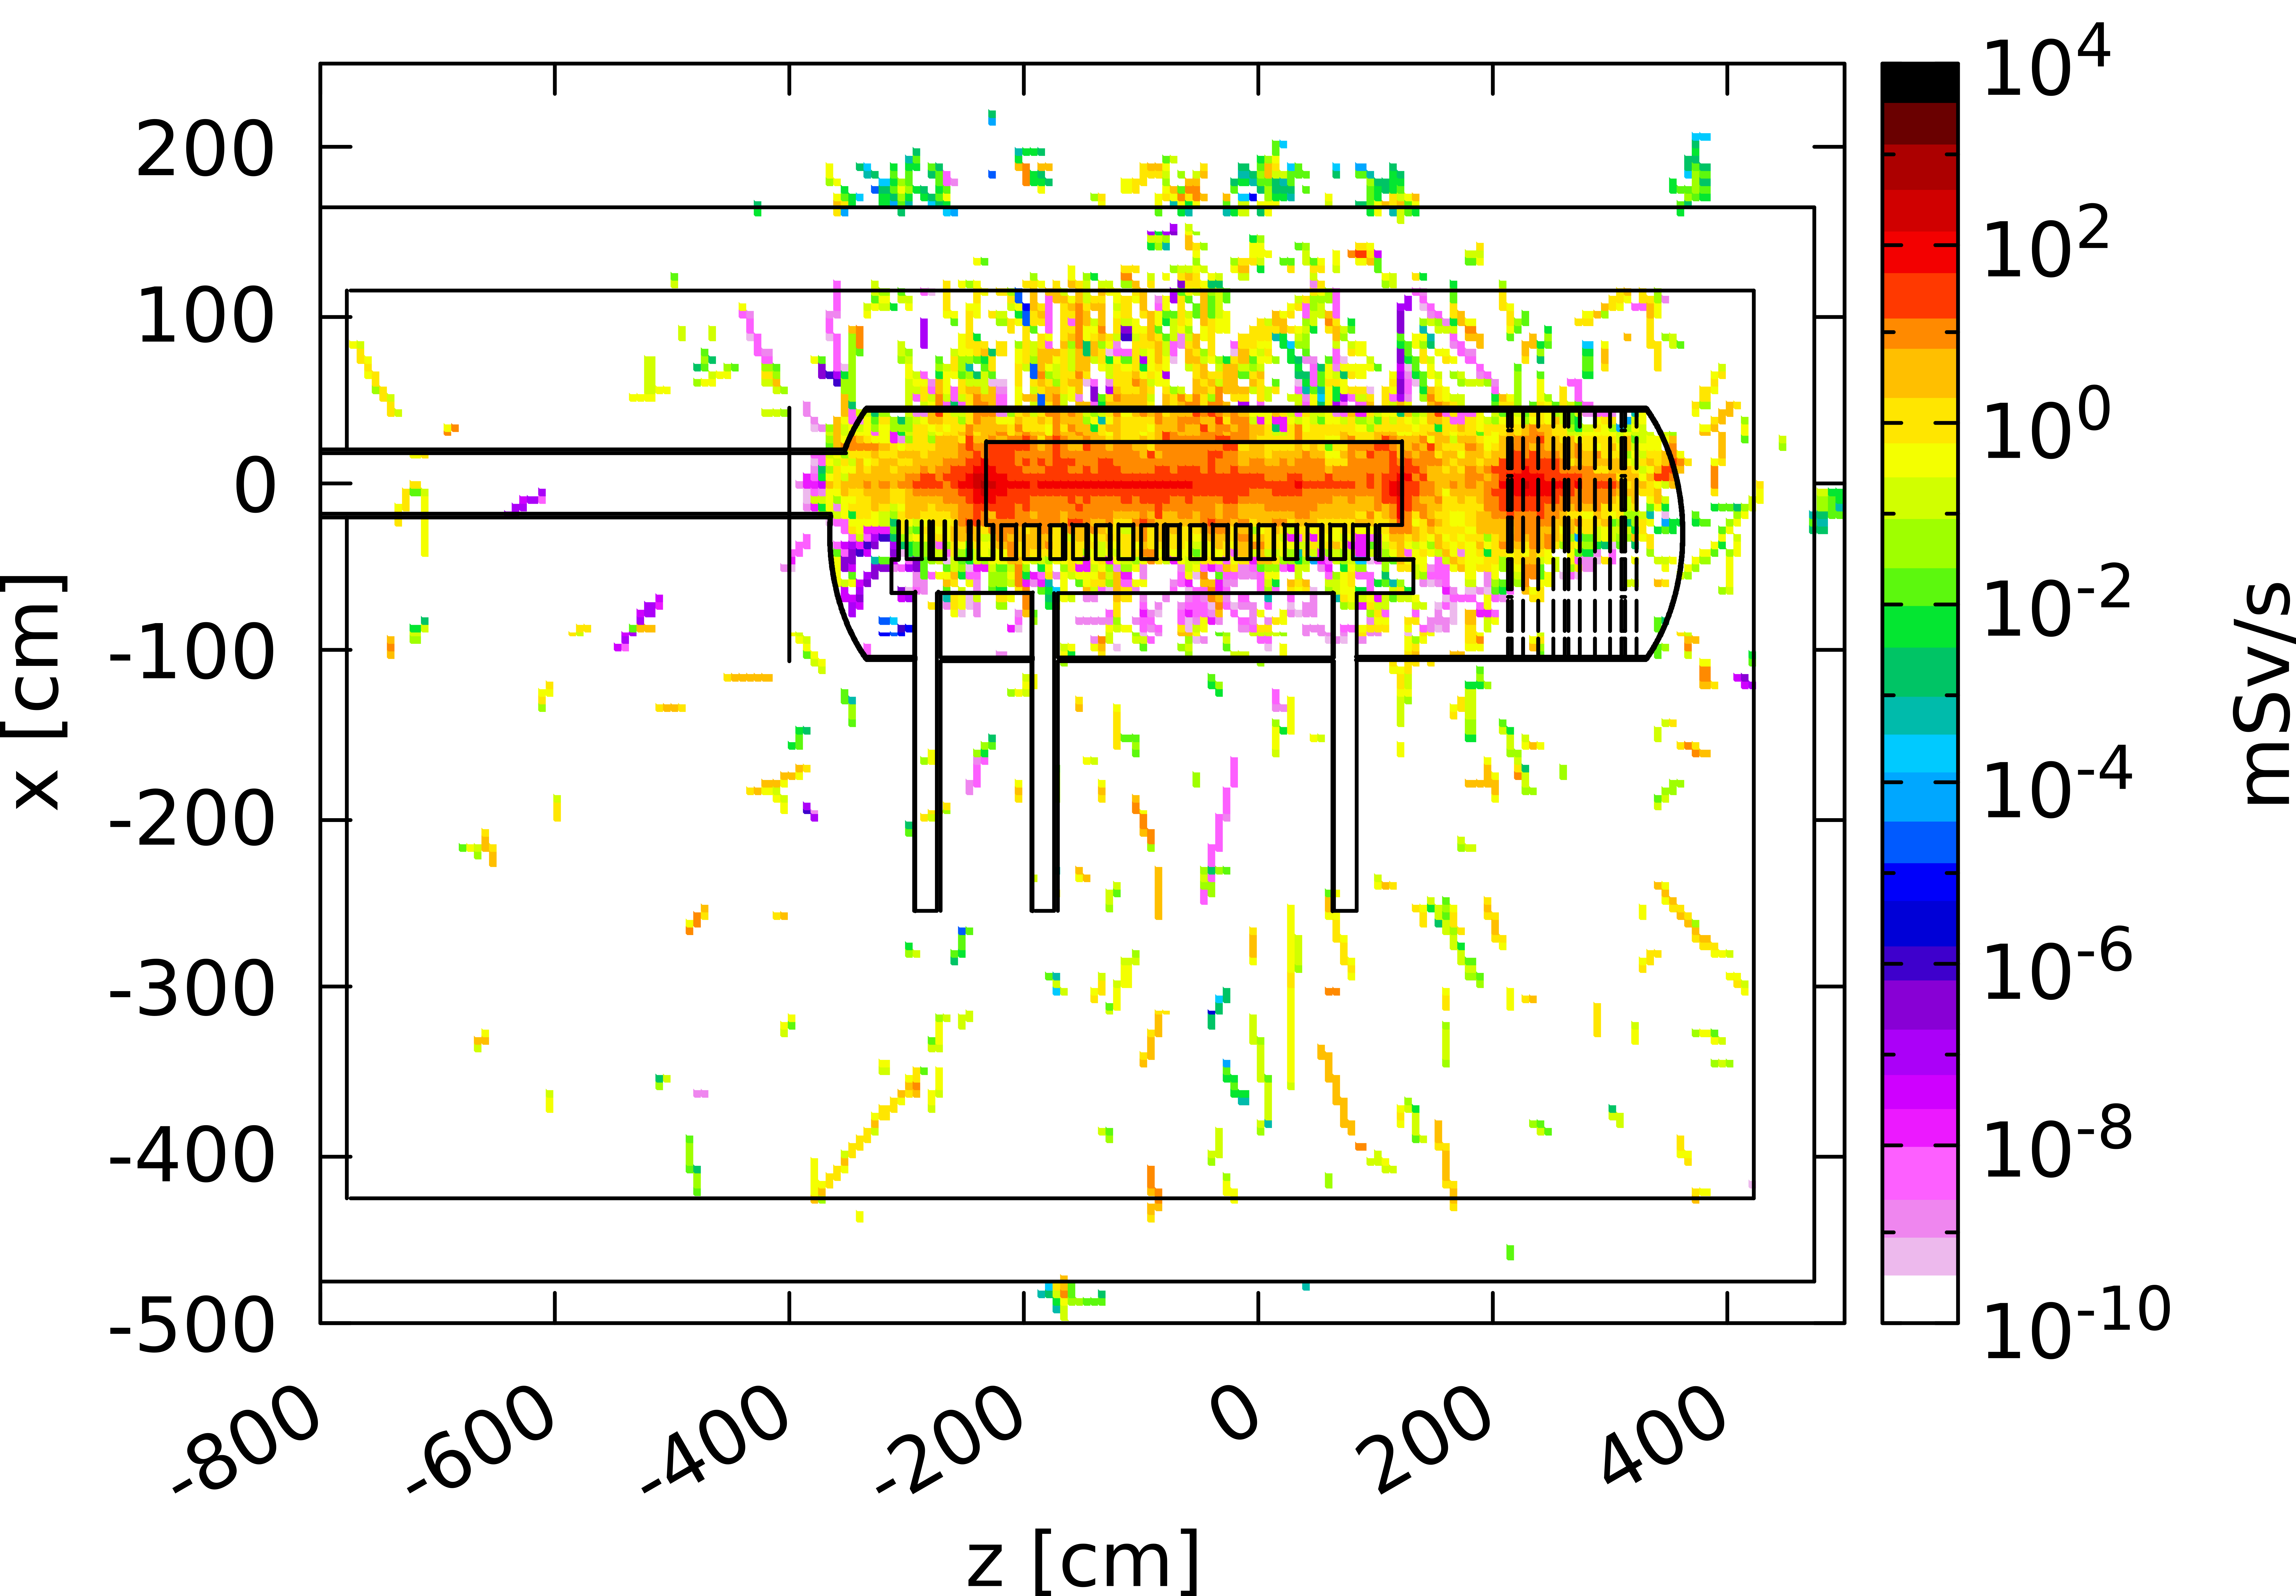
\includegraphics[width=\textwidth]{Figures/BeamDump/Design1_2.png}
   \caption{\designone, 1 hour}
   \end{subfigure}\\
     \begin{subfigure}[b]{0.49\textwidth}
   \centering
    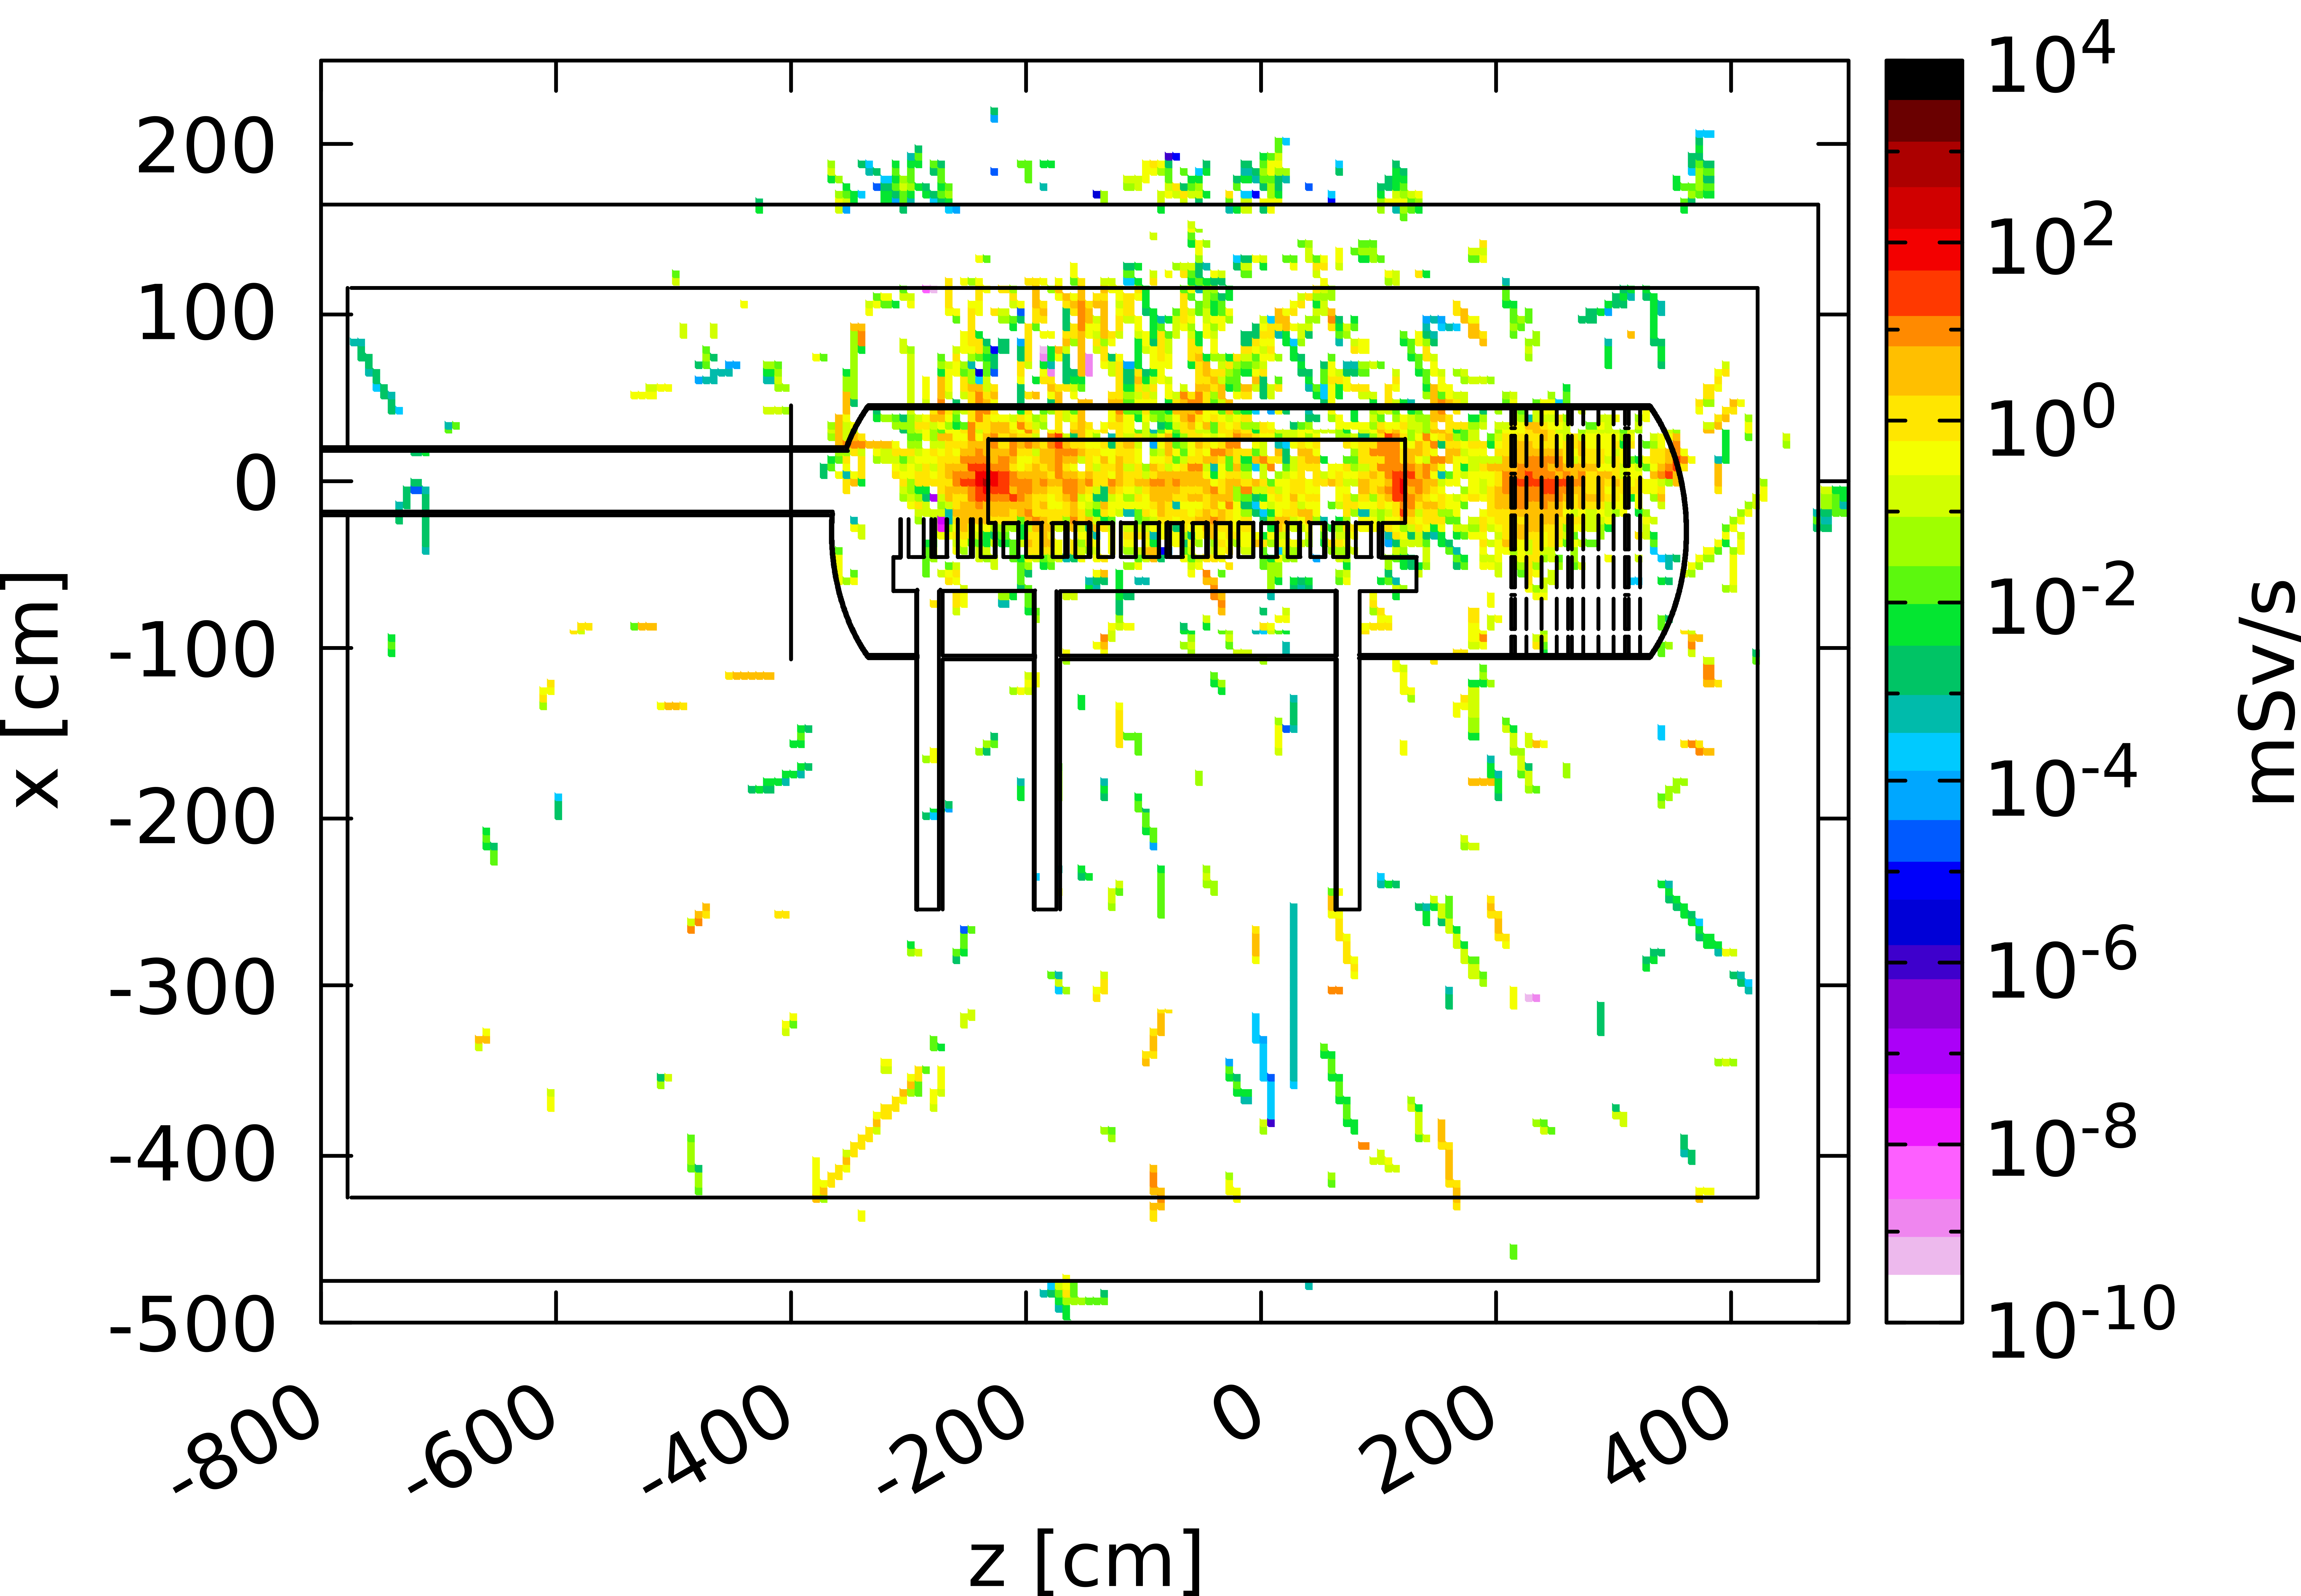
\includegraphics[width=\textwidth]{Figures/BeamDump/Design1_3.png}
   \caption{\designone, 1 day}
   \end{subfigure}
   \hfill
   \begin{minipage}{0.49\textwidth}
   \hfill
    \end{minipage}
    \caption[Dose rate in the ILC main beam dump \designone after cooling times]{\fluka result of the dose rate in the ILC beam dump \designone and their surrounding after one month of beam operation and certain cooling times.
   The cooling times are given in the captions of the individual subfigures.
   The view is in the xz plane of the beam dump surrounding including the shielding walls.
   The color scale shows the dose rate in \si{\milli\sievert\per\second}.}
   \label{fig:BeamDumps:DoseRate_Design1}
   \end{figure}
   \begin{figure}[htb]\ContinuedFloat
    \begin{subfigure}[b]{0.49\textwidth}
   \centering
    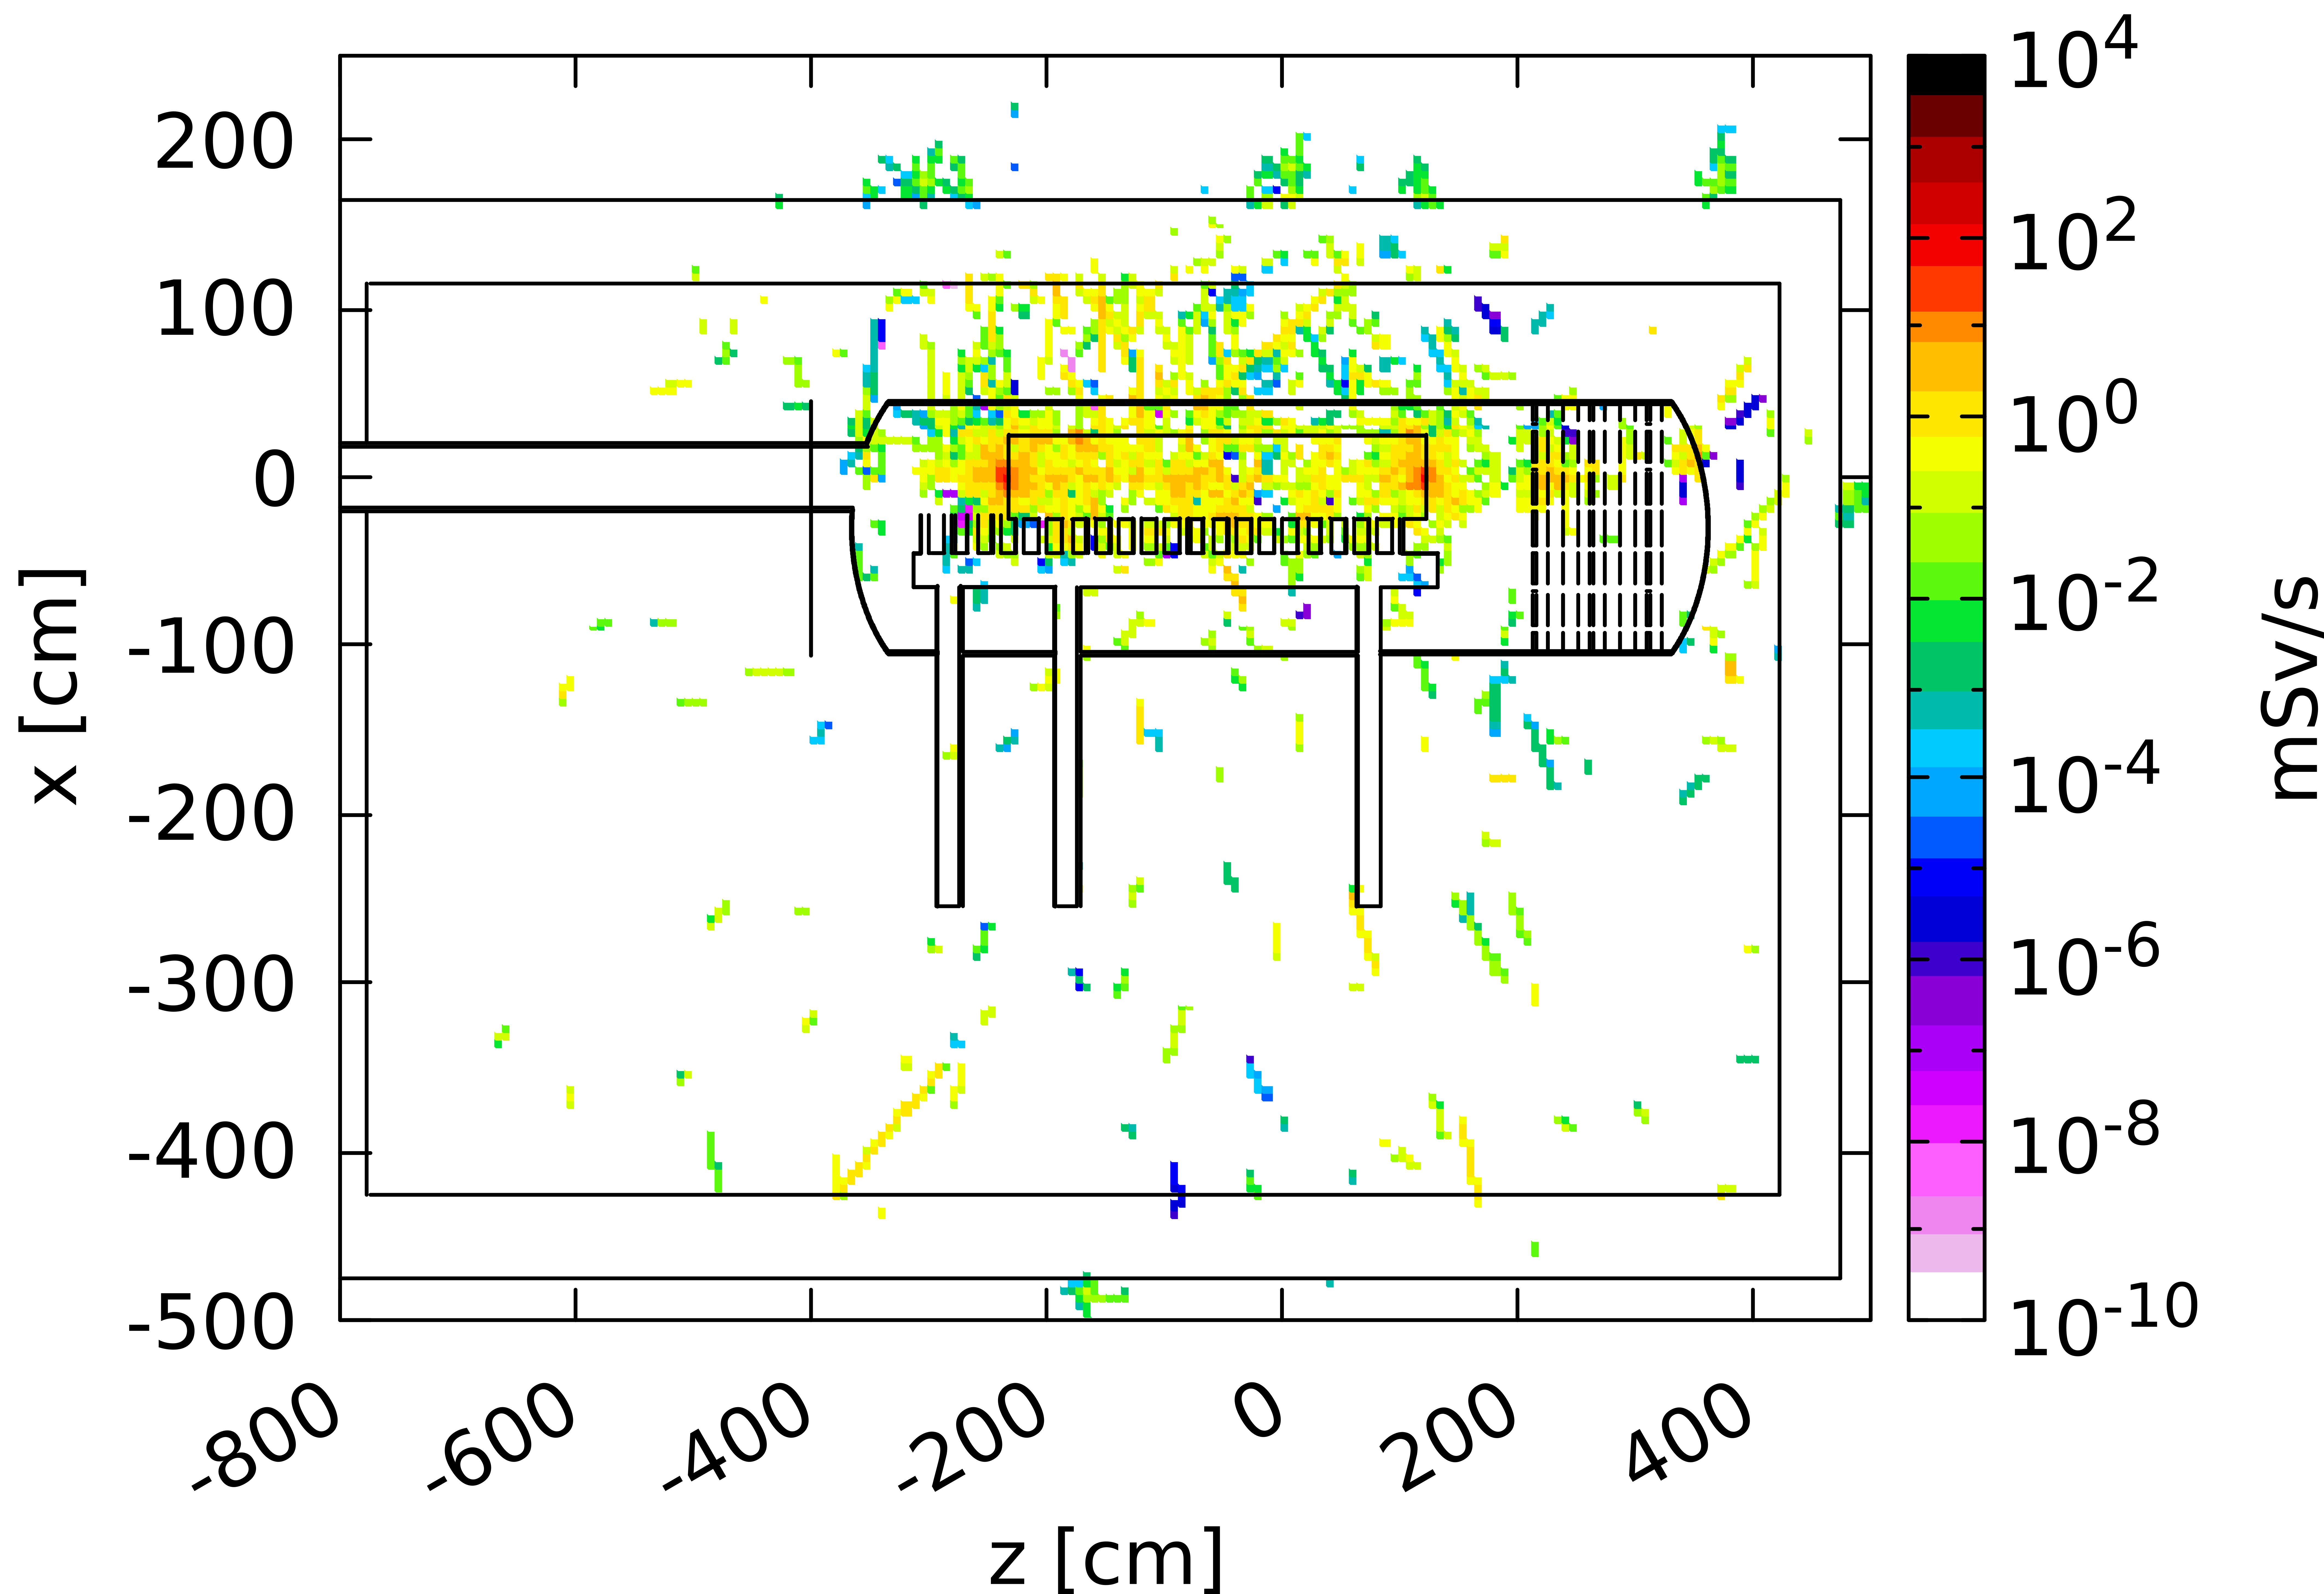
\includegraphics[width=\textwidth]{Figures/BeamDump/Design1_4.png}
   \caption{\designone, 1 month}
   \end{subfigure}
   \hfill
    \begin{subfigure}[b]{0.49\textwidth}
   \centering
    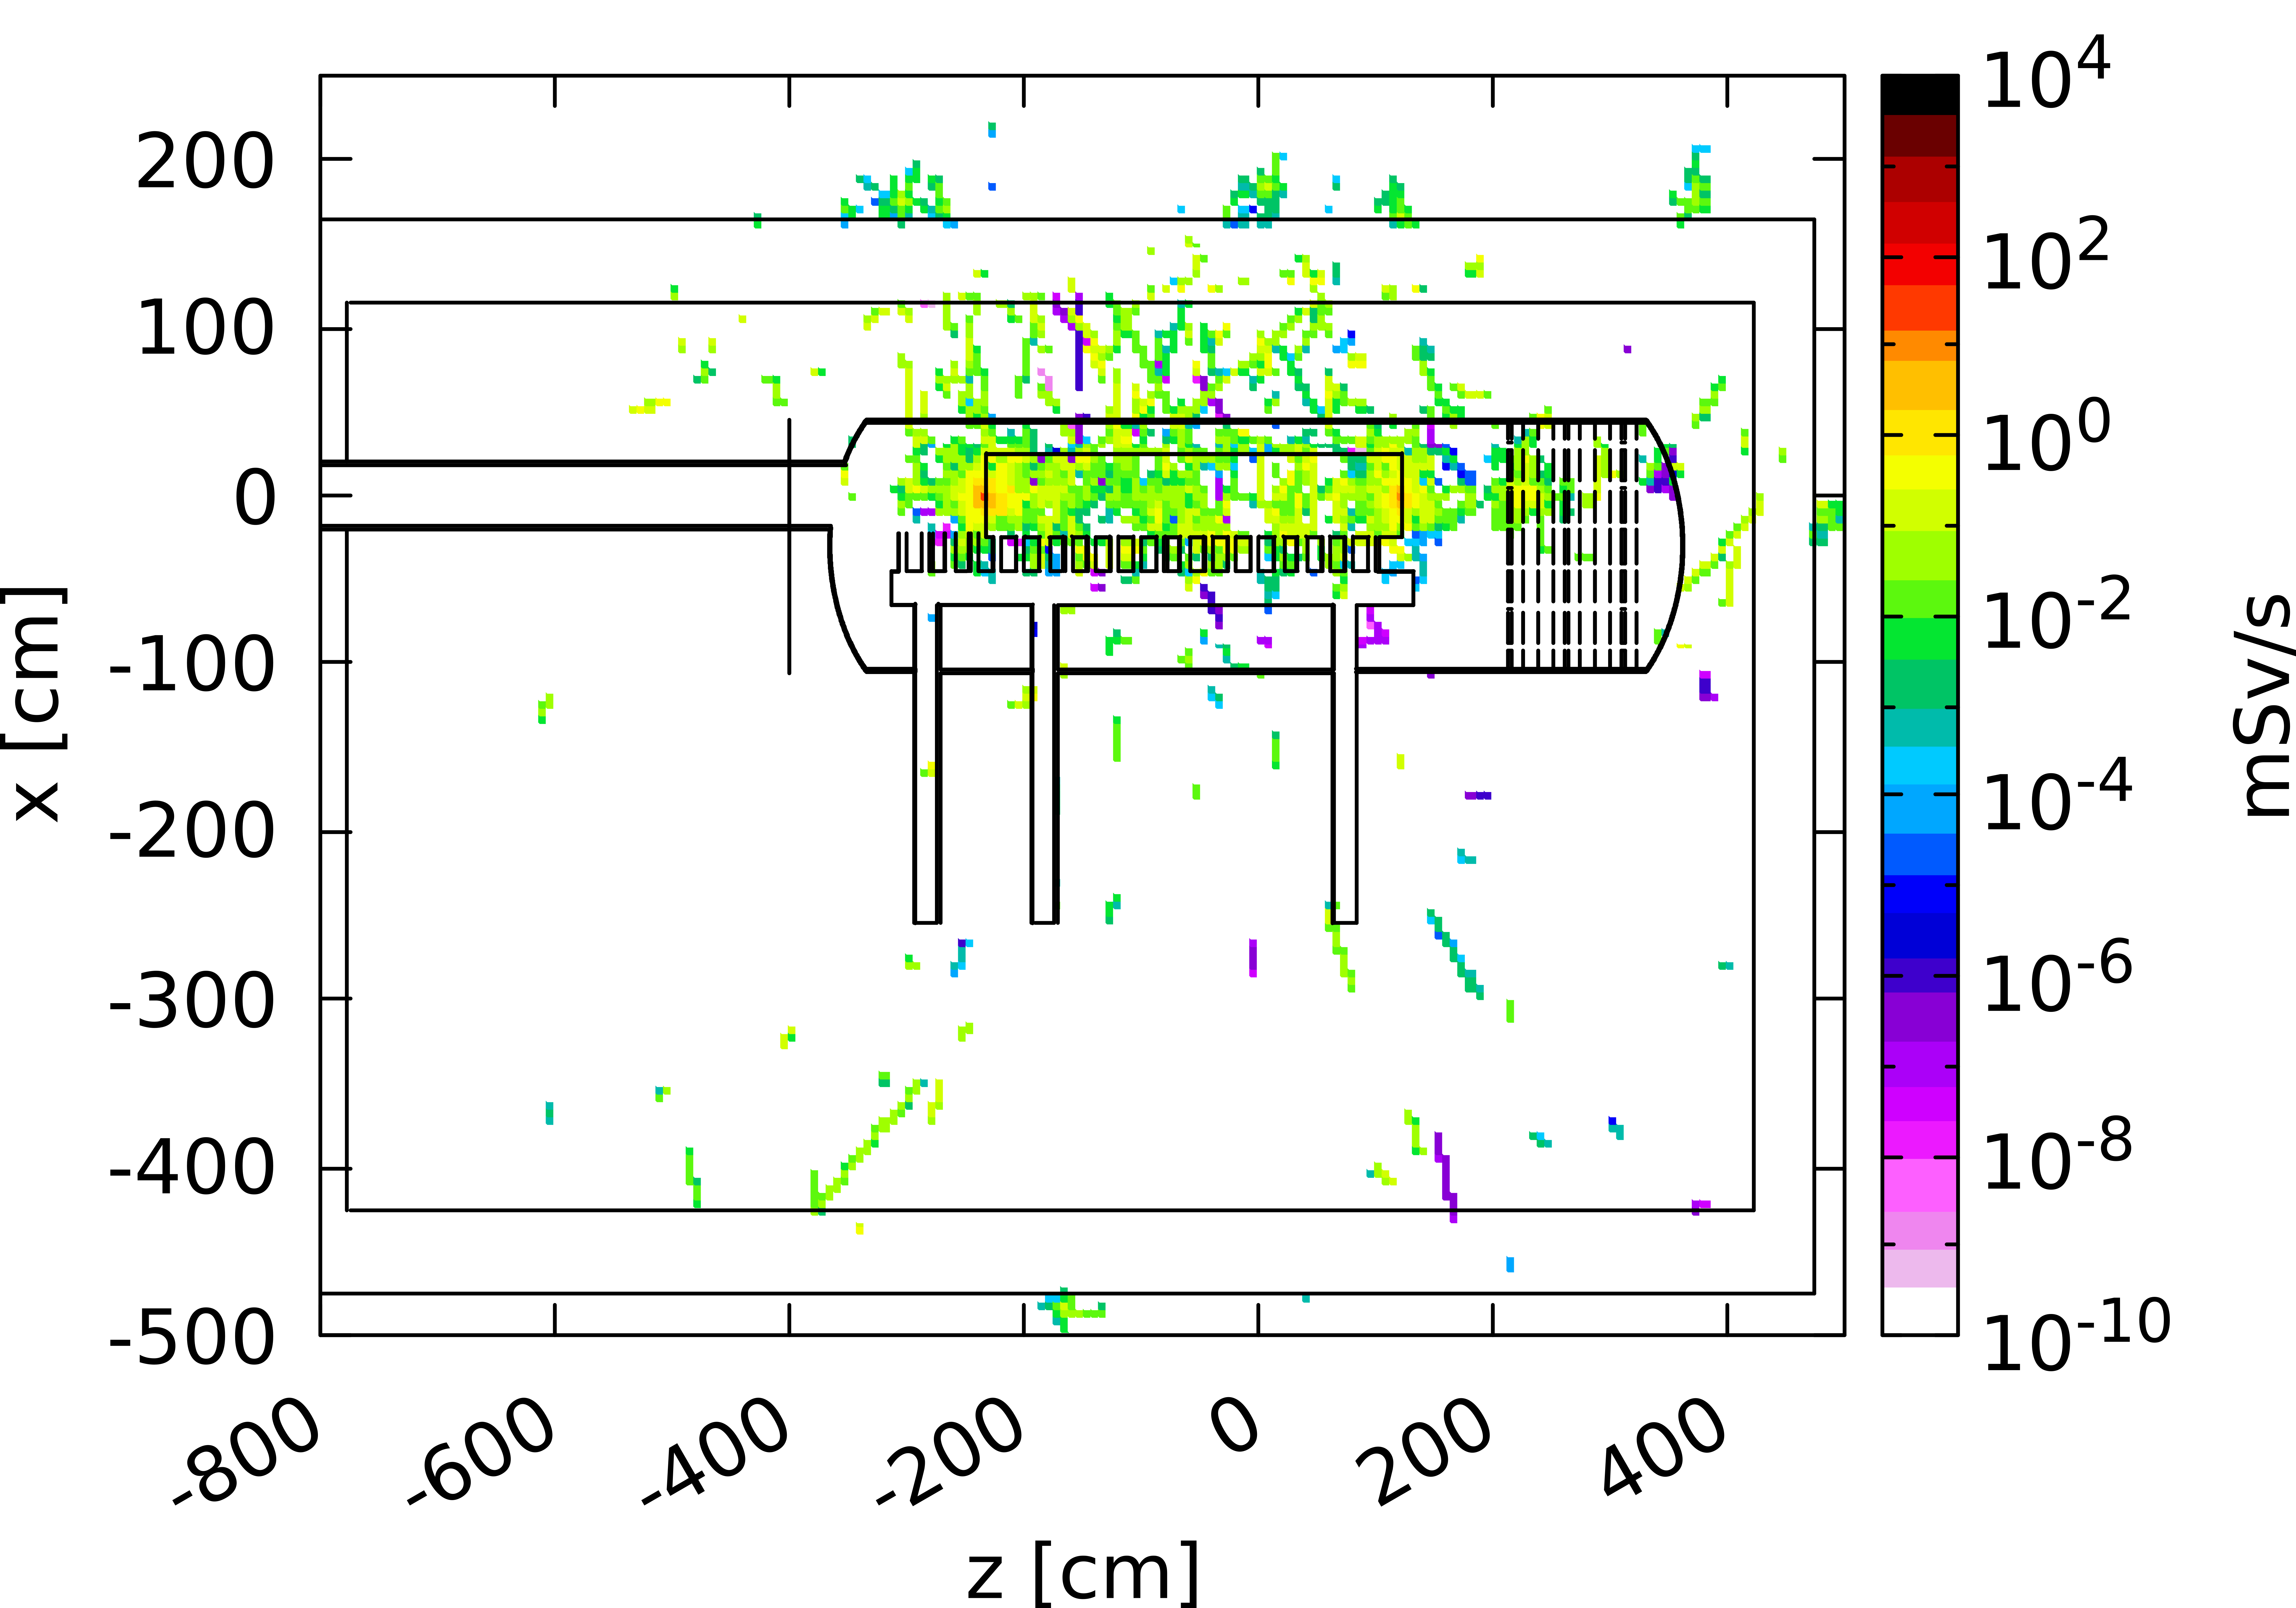
\includegraphics[width=\textwidth]{Figures/BeamDump/Design1_5.png}
   \caption{\designone, 1 year}
   \end{subfigure} 
       \caption[Dose rate in the ILC main beam dump \designone after cooling times]{\fluka result of the dose rate in the ILC beam dump \designone and their surrounding after one month of beam operation and certain cooling times.
   The cooling times are given in the captions of the individual subfigures.
   The view is in the xz plane of the beam dump surrounding including the shielding walls.
   The color scale shows the dose rate in \si{\milli\sievert\per\second}.}
   %\label{fig:BeamDumps:DoseRate_Design1}
\end{figure}



\begin{figure}
     \begin{subfigure}[b]{0.49\textwidth}
   \centering
    \includegraphics[width=\textwidth]{Figures/BeamDump/Design2_1.png}
   \caption{\designtwo, 1 minute}
   \end{subfigure}
   \hfill
    \begin{subfigure}[b]{0.49\textwidth}
   \centering
    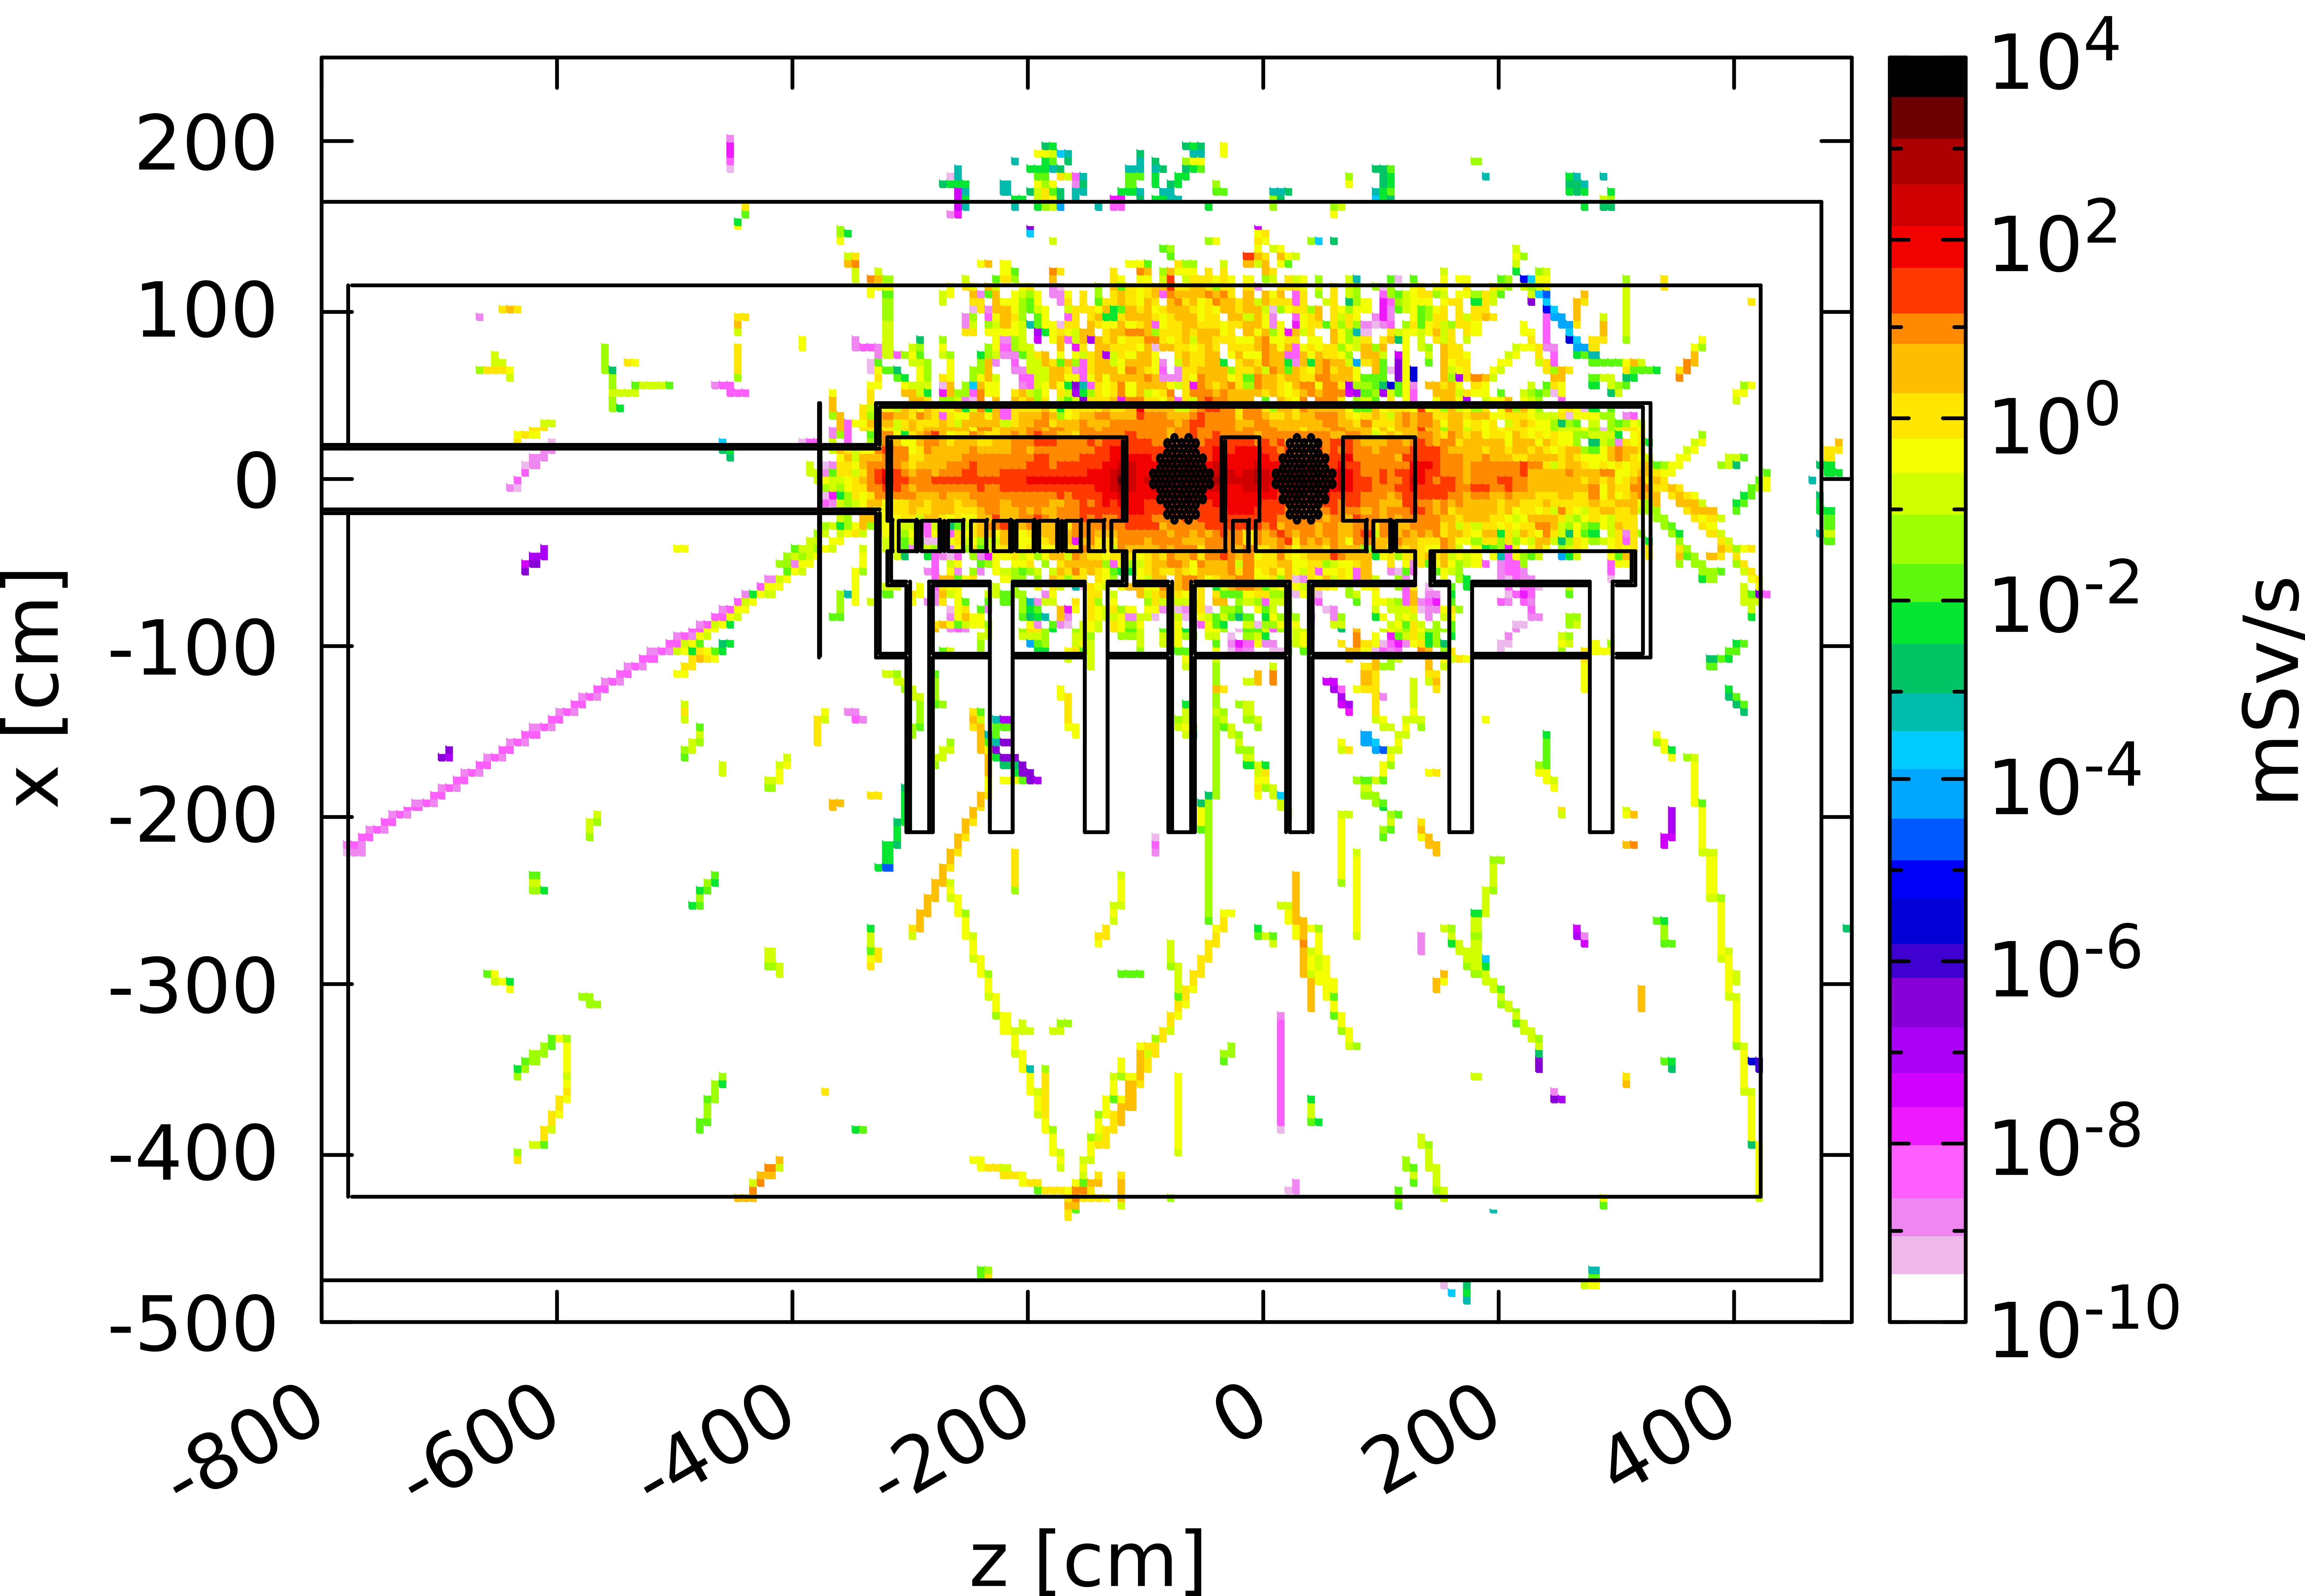
\includegraphics[width=\textwidth]{Figures/BeamDump/Design2_2.png}
   \caption{\designtwo, 1 hour}
   \end{subfigure}\\
     \begin{subfigure}[b]{0.49\textwidth}
   \centering
    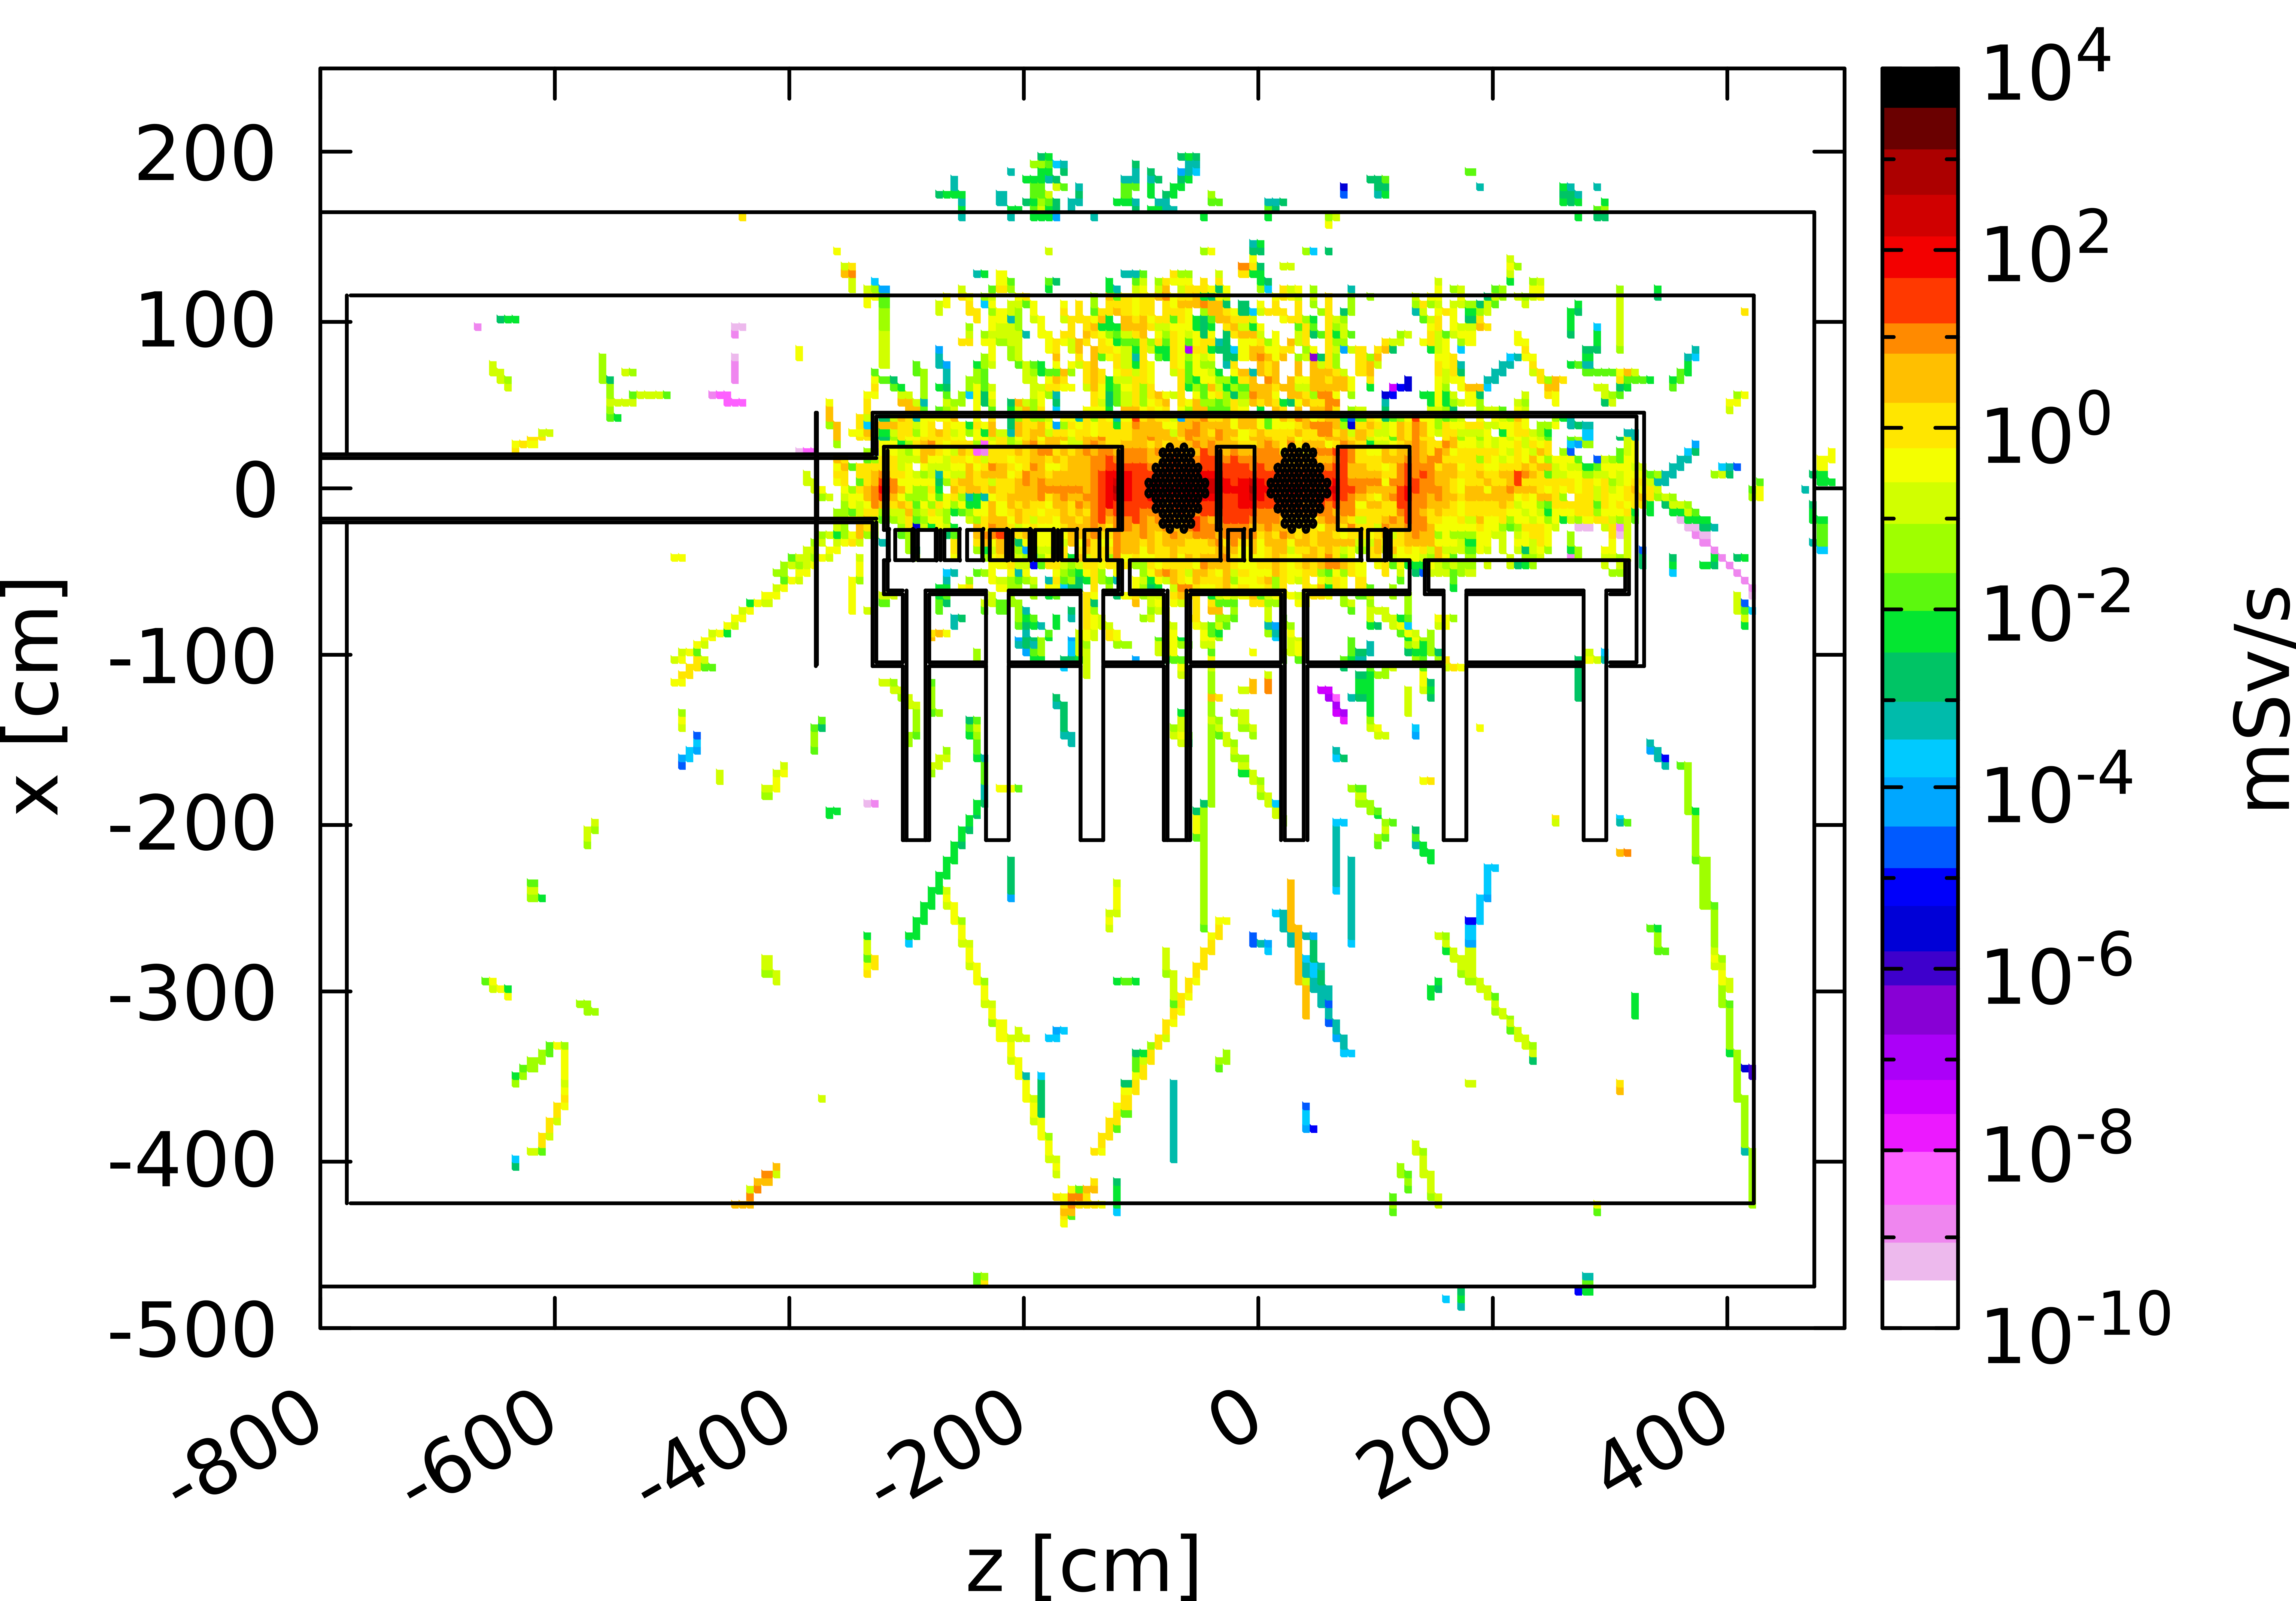
\includegraphics[width=\textwidth]{Figures/BeamDump/Design2_3.png}
   \caption{\designtwo, 1 day}
   \end{subfigure}
      \hfill
   \begin{minipage}{0.49\textwidth}
   \hfill
    \end{minipage}
   \caption[Dose rate in the ILC main beam dump \designtwo after cooling times]{\fluka result of the dose rate in the ILC beam dump \designtwo and their surrounding after one month of beam operation and certain cooling times.
   The cooling times are given in the captions of the individual subfigures.
   The view is in the xz plane of the beam dump surrounding including the shielding walls.
   The color scale shows the dose rate in \si{\milli\sievert\per\second}.}
   \label{fig:BeamDumps:DoseRate_Design2}
      \end{figure}
   \begin{figure}[htb]\ContinuedFloat
    \begin{subfigure}[b]{0.49\textwidth}
   \centering
    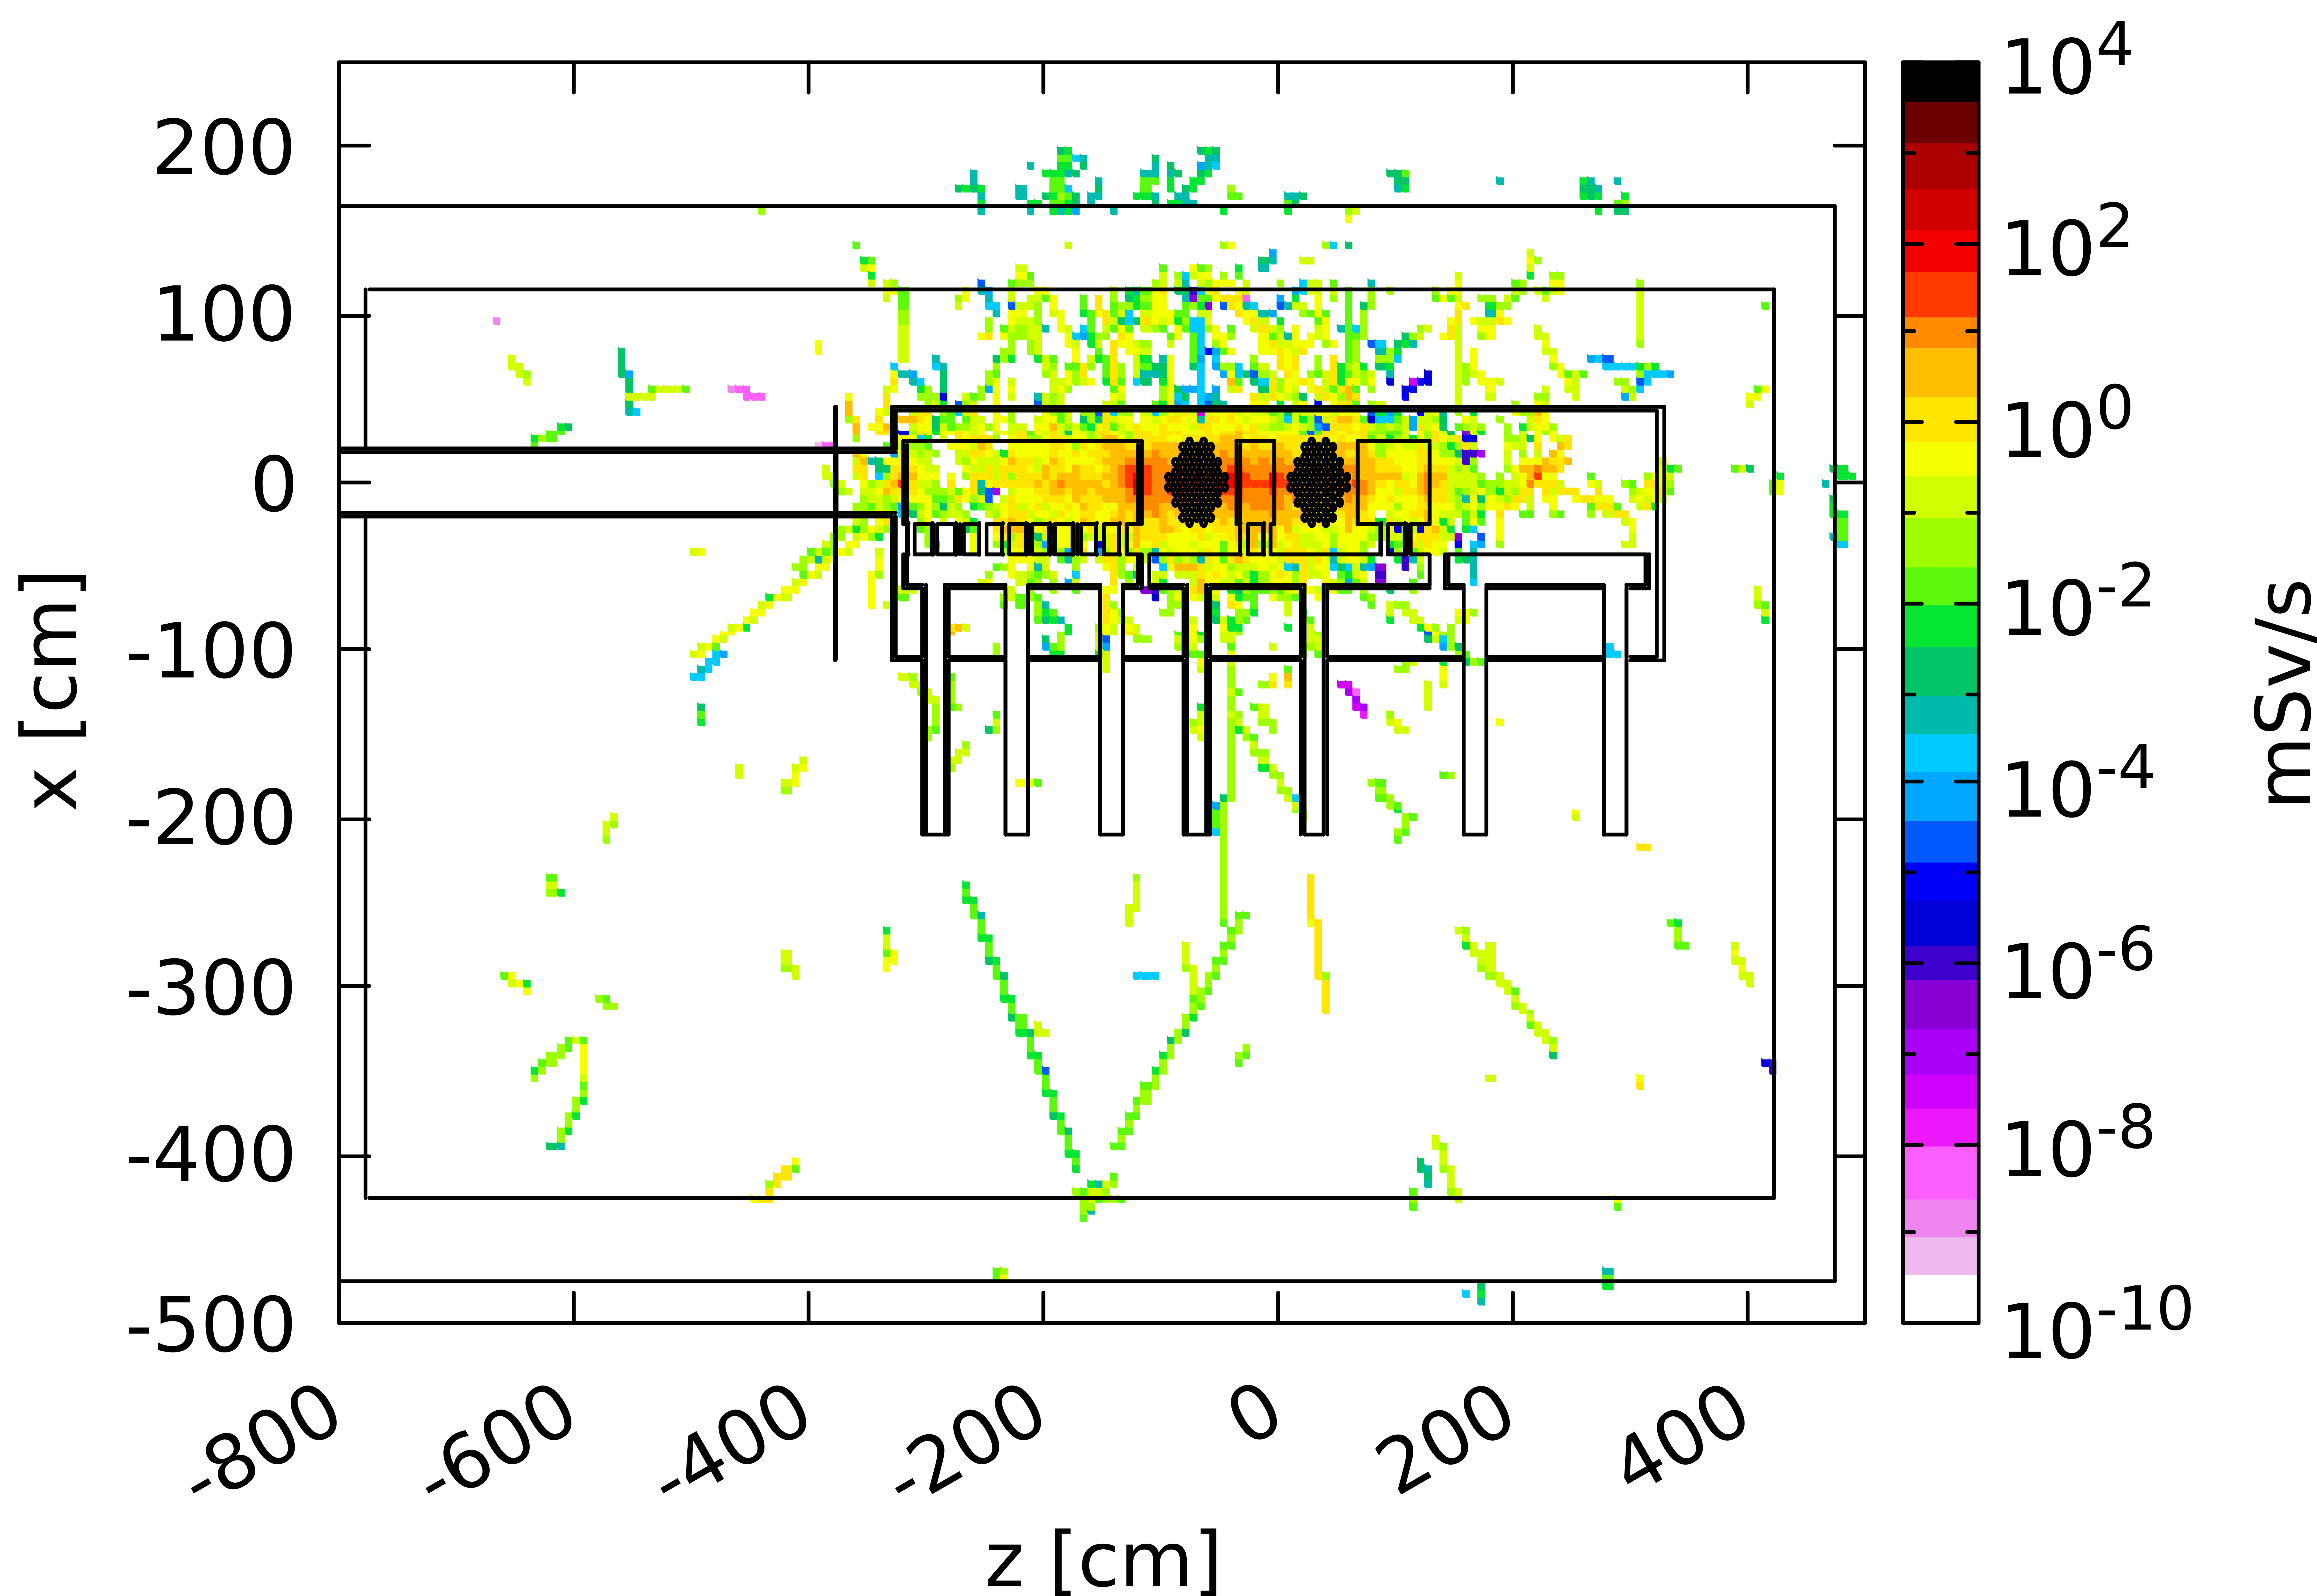
\includegraphics[width=\textwidth]{Figures/BeamDump/Design2_4.png}
   \caption{\designtwo, 1 month}
   \end{subfigure}
   \hfill
    \begin{subfigure}[b]{0.49\textwidth}
   \centering
    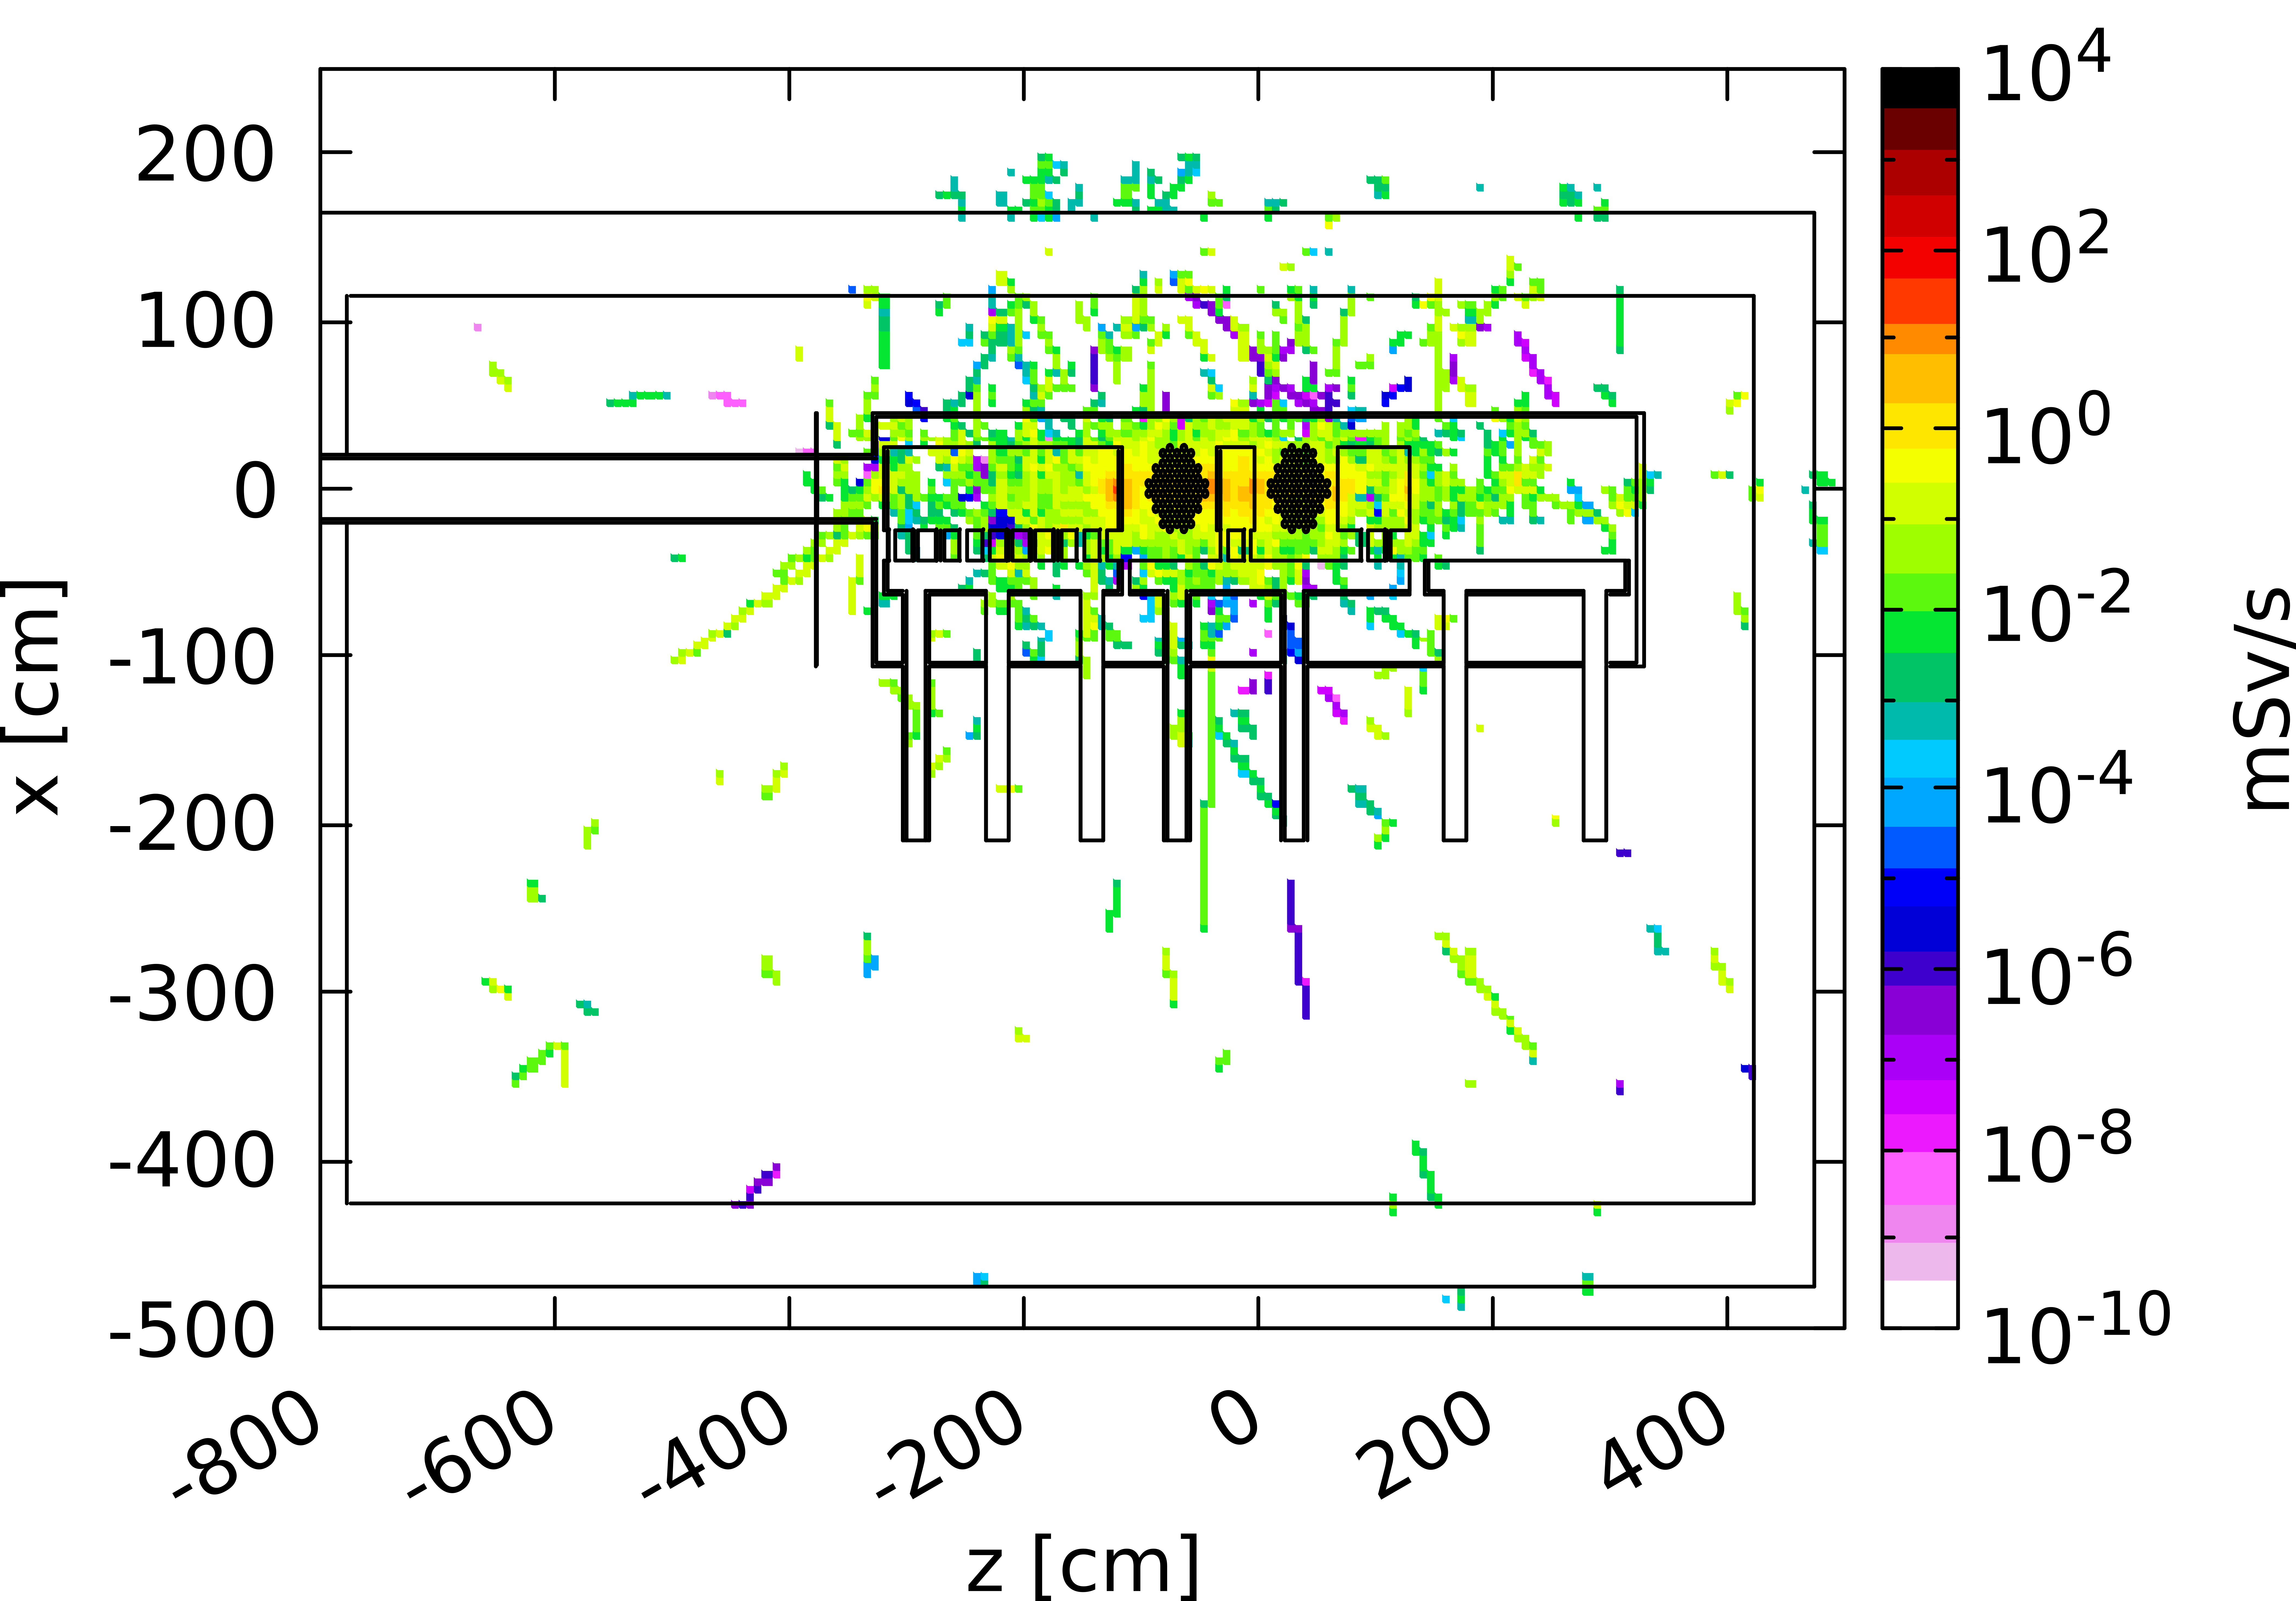
\includegraphics[width=\textwidth]{Figures/BeamDump/Design2_5.png}
   \caption{\designtwo, 1 year}
   \end{subfigure}
   \caption[Dose rate in the ILC main beam dump \designtwo after cooling times]{\fluka result of the dose rate in the ILC beam dump \designtwo and their surrounding after one month of beam operation and certain cooling times.
   The cooling times are given in the captions of the individual subfigures.
   The view is in the xz plane of the beam dump surrounding including the shielding walls.
   The color scale shows the dose rate in \si{\milli\sievert\per\second}.}
   %\label{fig:BeamDumps:DoseRate_Design2}
\end{figure}